\documentclass[11pt,fleqn,twoside]{book}

%
%   If twoside is specified, headers alternate and a blank
%   page is inserted between cover and titlepage (useful for a5)
%   
%   set the languages (last should be the one of the main text; e.g.,
%   german, english)
%   and  include the style:
%

% Switch for report-text / paper-text 
\newif\ifreport
\reporttrue

\usepackage[utf8]{inputenc}

\usepackage[final]{pdfpages}
\usepackage{verbatim}

\usepackage[english]{babel}
\usepackage{derireport}

\usepackage{epsfig}
\usepackage{url}
\usepackage{times}
\usepackage{alltt}
\usepackage{xspace}
\usepackage{latexsym}
\usepackage{rotating}
\usepackage{numprint}

\usepackage{graphicx}
\usepackage{epstopdf}
\usepackage{float}
\usepackage{multirow}
\usepackage{paralist}
\usepackage{booktabs}
\usepackage[lined,algoruled,linesnumbered,english]{algorithm2e}
\usepackage[dot,dash]{dashundergaps}
\usepackage{framed}

\usepackage[colorlinks=true]{hyperref}
\usepackage{pgfplots}
\usepackage{tikz}
\usepackage{amssymb}
\usepackage{amsthm}
\usepackage{amsmath}
\usepackage[toc,page]{appendix}
\usepackage{subfig}
\usepackage{listings}

\newfloat{fileformat}{thp}{lof}[section]
\floatname{fileformat}{File Format}

\lstset{
  basicstyle=\scriptsize\ttfamily,
  tabsize=2,
  breaklines=true,
  columns=fullflexible,
  keywordstyle=\color[rgb]{0,0,1},
  commentstyle=\color[rgb]{0.133,0.545,0.133},
  stringstyle=\color[rgb]{0.5,0.5,0.5},
  captionpos=b
}
\lstloadlanguages{Java,XML}

% Used in benchmark tables
\newcommand{\ra}[1]{\renewcommand{\arraystretch}{#1}}
\newcommand{\hs}{\hspace{0.042in}}
\newcommand{\whs}{\hspace{0.25in}}
\renewcommand{\lstlistlistingname}{List of Listings}

\foreignreport

 \newtheorem{theorem}{Theorem}[section]
 \newtheorem{proposition}[theorem]{Proposition}
 \newtheorem{corollary}[theorem]{Corollary}
 \newtheorem{lemma}[theorem]{Lemma}

 \newtheorem{example}{Example}[section]
 \newtheorem{definition}{Definition}[section]

%\newcommand{\qed}[0]{\hspace*{1em}\hbox{\proofbox}}

% \newtheorem{zdefinition}{Definition}[section]
% \newenvironment{definition}[1][\mbox{}]{\begin{zdefinition}\begin{rm}#1}{\end{rm}\end{zdefinition}}

% \newtheorem{zexample}{Example}[section]
% \newenvironment{example}[1][\mbox{}]{\begin{zexample}\begin{rm}#1}{\end{rm}\end{zexample}}


 %% No numbered paragraphs
 \setcounter{secnumdepth}{3}

%%%%%%%%%%%%%%%%%%%%%%%%%%%%%%%%%%%%%%%%%%%%%%%%%%%%%%%%%%%%%%%%%%%%%%%%%%%%%%%%%%



%
% This is the title of the report, shown on the cover: 
%

\title{%
Compression Techniques for Inverted Lists in Web Search Engines.
\vskip 1em 
Inverted Lists Structure for Semi-Structured Web Data Search.
}

\authornames{Campinas St\'ethane}


\innertitle{}

%  The authors appear with affiliations. 
%  Thanks may be given for individual acknowledgements.

%\author{
%Campinas St\'ephane%
% \affiliation{
% DERI (Digital Enterprise Research Institute), National University of Ireland,
% Galway\protect, IDA Business Park, Lower Dangan, Galway, Ireland.
% \mbox{E-mail: stephane.campinas@deri.org.}}
%}

%
% Publication information about preliminary version, if any
% Optional.
%

% \published{Preliminary results of this paper appeared in ``Applications of 
% Modal Logics in Interstellar Travelling'' 
% {\em Proceedings of the First Interstellar Workshop on Paranormal Logics, 
% March 24--25}, Lecture Notes in Science Fiction 0815,
% Springer, 1974,  pp.\ 1--10.
% }

% General acknowledgements, appearing only on the inside titlepage.
% Must be one continuous paragraph. 
% If you want to make two or more paragraphs, 
% use \\*[\parskip] for new line, but do not leave a line empty.
%

\acknowledgement{
\\*[\parskip]
The author wishes to thank his supervisors, Giovanni Tummarello and Renaud
Delbru, for making this internship possible. The author wishes to thank
also Renaud Delbru for providing a constant help and giving excellent
instructions as well as an interesting view of the research world. The author
also wants to thanks the EPITA teacher for the preparation during the the
school year.
\\*[\parskip]
The author wishes further to thank his family and Katarzyna Osuchowska for
their continuous support. }

%
% Abstract must also be one continuous paragraph. 
% If you want to make two or more paragraphs, 
% use \\*[\parskip] for new line and \hspace*{1.5em} for indentation, 
% but do not leave a line empty.
%

\abstract{%
\\*[\parskip]
The Semantic Web is a set of layers that wraps the current web and adds useful
meta-information describing web documents' content. This semantic information
has a structured format, allowing web documents to be exploitable by humans and
machines alike. In the latter case, machines permit a more comprehensive use of
the colossal amount of knowledge in the Web. The number of such documents can
already be counted in millions and is increasing rapidly. This calls for large
scale systems that are able to search through this data and to retrieve
relevant information. This report highlights that the time spent on IO
operations for such systems is wasted, and thus reviews two approaches to
answer this problem. We propose a compression method that increases both the
update and the query throughput of the system. We introduce also a model that skips
over data, avoiding to read unnecessary data.
}

%
% The following data can be specified by either the author(s) 
% or by the system administrator after submission:
%

\deritr{\today}
% Give different versions separated by semicolon:
%\date{December 2010}

%
% If \date{} is missing, the current date in format: 
%   <month> - <year> 
% is chosen. 
% Using \fulldate, the format 
%   <month> - <day>, <year> (english) 
% resp.
%      <Tag>. <Monat> <Jahr>
% is chosen.
%

% Start the document here ...
% (Macros, etc)

\begin{document}
%
% the next line MUST come first 
%

\maketitle

\newpage 
\pagenumbering{Roman}

{\small
%\vspace*{-3.5\baselineskip}

\tableofcontents
}
%\cleardoublepage

\newpage
\pagenumbering{arabic}

%
% Here starts the body of the paper ...
%
%%%%%%%%%%%%%%%%%%%%%%%%%%%%%%%%%%%%%%%%%%%%%%%%%%%%%%%%%%%%%%%%%%%%%%%%%%%%%%
\part{Prelude}%
%%%%%%%%%%%%%%%%%%%%%%%%%%%%%%%%%%%%%%%%%%%%%%%%%%%%%%%%%%%%%%%%%%%%%%%%%%%%%%
\label{sec:prelude}
\chapter{Introduction}{
The Web as we know it is mostly a huge collection of documents, e.g. texts,
pictures, \ldots, connected together thanks to HTTP links.
These links carry no meaning about the
relationship between two documents, or about the content a document exhibits.
Linked Data refers to those same documents, but enriched with \emph{semantic}
meta-data. For example, the content of a document can be described by this
meta-data by indicating the language it was written in, or the content's type,
e.g. book or article. Tim Berners-Lee has first introduced the idea of such
enriched web documents, called \emph{Linked Data}. For such a vision to be
viable as the web is now a large collection of heterogeneous data, a framework
that sets the best practices for publishing and searching Linked Data is a
necessity. The \emph{Semantic Web} is such a framework and is not aimed to be a
replacement of the Web as we know it, but as an extension giving relevant
knowledge about documents on the web.
\linebreak

Over the past years, the quantity of Linked Data available has been increasing
and is now reaching a climax. Semantic Data now at hand, the challenge is to be
able to search for information efficiently. Linked Data is commonly stored
within databases called \emph{Triple Stores}, where querying is normally done
thanks to the standardized query language SPARQL defined with the Semantic Web.
However this language, while being very expressive, is known not to scale
efficiently to a large amount of data. \emph{SIREn} is an Information
Retrieval-based search engine which goal is to store and to query efficiently
at the web scale Linked Data. SIREn is a low level application, meant to be
used by other applications such as web services that provide people
information results about what they queried for. \emph{Sindice} is a web
service that provide people and machines a search engine over Linked Data
through the use of SIREn.
\linebreak

SIREn builds an index over the Linked Data collections for searching and
retrieval purpose. With the amount of Linked Data growing quickly, the size of
such indexes and the performance to retrieve data from it are then points of
interest to build a scalable system. A compressed index is of course important
in order to take less space, however decreasing the time spent on IO operations
is also important in order to increase the query throughput. Within the long
studied domain of Information Retrieval, compression methods have been
developed for that purpose. However they were built for traditional indexes,
i.e., indexes built on collections with textual documents (unstructured data). On
the contrary, SIREn builds indexes on Linked Data, i.e., (semi) structured
data. Because the type of data differs, the model used to index documents
is different, which implies that the distribution of indexed values are
different. State of the art compression techniques are not adapted to this new
distribution of values, and so a new compression class has been developed to
match this need: \emph{Adaptive Frame Of Reference}.
\linebreak

Index compression is one aspect that has to be taken care of when building an
efficient and scalable Information Retrieval search engine. Some information
in the index is not relevant to a query. Reading unnecessary data when
processing a query is then wasted time. An other aspect to optimize the
performance of a search engine is to avoid reading useless information with
regards to a query as much as possible by using \emph{self-indexing}
techniques. The \emph{Skip Lists} is a data structure that can be used for that
purpose. Highly efficient compression techniques are nowadays block-based
algorithms. However Skip Lists abstracts from the block view, discarding
statistics about the block that could be used for a more efficient structure.
\emph{SkipBlock} is a block-based self-indexing model that generalizes the
Skip Lists structure.

We review in this report some techniques that aim to reduce the IO access time
overhead in order to increase the overall performance of the Information
Retrieval web search engine. We present AFOR, a compression method that
provides both fast compression and decompression speed, and yet with a high
compression ratio. We propose SkipBlock, a new self-indexing model that
reduces the time of random lookups from inverted lists. }
\section{Motivation}

\subsection{Semantic Web}

\begin{framed}
\begin{quote}
I have a dream for the Web [in which computers] become capable of analyzing
all the data on the Web – the content, links, and transactions between people
and computers. A ``Semantic Web'', which should make this possible, has yet to
emerge, but when it does, the day-to-day mechanisms of trade, bureaucracy and
our daily lives will be handled by machines talking to machines. The
``intelligent agents'' people have touted for ages will finally materialize.
\end{quote}
– Tim Berners-Lee, 1999
\end{framed}

The Semantic Web is an extension of the current Web and acts as a layer of
resource descriptions on top of the current one. These descriptions are
metadata, data about data, that specify various information about web
resources such as their author, their creation date, the kind of the content,
\ldots. Within the Semantic Web framework, \emph{Resource Description
Format}\footnote{\url{http://www.w3.org/TR/2004/REC-rdf-concepts-20040210/\#section-Concepts}}
(RDF) is a standard format that is used to describe a document. RDF adds
information about a web document by embedding metadata. RDF data is structured
data\footnote{Structured data follow a strict a format that allows machine to
understand and process it.}. However semantic data on the Web is large, and each
dataset may have its own schema that may be partially known. They do not all
follow a rigid structure as in databases. We say that the data is
\emph{semi-structured} \cite{abiteboul:1997:icdt}.

Over the past few years, an increasing quantity of Semantic data has been
published on the web, and not just by some programmers but also by industries,
governments and individuals. Some recent RDF data published are:
\begin{itemize}
  \item Governments provide their information to citizens thanks to Linked
  Data such as the British dataset \url{http://data.gov.uk/}, or
  \url{http://data.gov/} by the USA government.
  \item News agents such as the New York Times or Reuters include semantic
  information (i.e., RDF) in their articles.
  \item Web content management systems like Drupal that ease the process to
  expose one's data as structured information for the Semantic Web.
  \item BestBuy\footnote{BestBuy: \url{http://www.bestbuy.com/}} which publishes
  product descriptions, store details and other information in a machine-readable
  format.
\end{itemize}
As per Tim Berners-Lee quote, the semantic web is becoming a reason to get
things moving. The
article\footnote{``The Web Turns 20: Linked Data Gives People Power, Part 1 of
4'' article, which can be found at the address 
\url{http://www.scientificamerican.com/article.cfm?id=berners-lee-linked-data}}
relates some of the possibilities the semantic web gives. It reports that it
allows people to get more involved with the government, e.g. by publishing on
what the public money is being spent on.

\subsubsection{Semantic Web in Action}

A lot of effort has been put in building a set of best practices to make the
Semantic Web viable. This section shall give an overview of this work by first
reviewing prominent ontologies that have been developed to describe knowledge
for a specific domain. Finally we will show an application use case based on Sindice,
called \emph{Sig.ma}, that aggregates Linked Data from different datasets into
one single ``entity profile'', i.e., all resources related to a same entity,
for example such as the entity DERI.

\subsubsection{Publishing Semantic Data}

Tim Berners-Lee, the person credited with coining the terms Semantic Web and
Linked Data, has frequently described Linked Data as ``the Semantic Web done
right''\footnote{slides: \url{http://www.w3.org/2008/Talks/0617-lod-tbl/\#(1)}}.
It aims to create different semantic data datasets of knowledge and to connect
them together. The we can perform a search on a particular dataset, and then to
move to an other dataset because it is somehow related to the current one.
Through a 5-stars Linked Data publishing scheme, Tim Berners-Lee sets the
steps to follow so that individuals and government people contribute in a good
way to enrich the semantic data collection:
\begin{description}
  \item[$\star$] Available on the web (whatever format), but with an open licence
  \item[$\star\star$] Available as machine-readable structured data (e.g. excel
  instead of image scan of a table)
  \item[$\star\star\star$] as (2) plus non-proprietary format (e.g. CSV instead
  of excel)
  \item[$\star\star\star\star$] All the above plus, use open standards from
 W3C\footnote{The World Wide Web Consortium, W3C: \url{http://www.w3.org/}, is
 an international community to build Web standards}, (RDF and SPARQL) to
 identify things, so that people can point at your stuff
  \item[$\star\star\star\star\star$] All the above, plus: Link your data to
  other people’s data to provide context
\end{description}

The Open Data Movement aims at making web data freely available to everyone. The
goal of the Linking Open Data community project is to extend the Web with a
data commons by publishing various open data sets as RDF on the Web and by
setting RDF links between data items from different data sources. RDF links
allow people, and even more so machines, to navigate through the heterogeneous
information. Web data is represented using standard technologies, allowing
data to be reused across applications. The Figure~\ref{fig:LOD} depicts the
current state of the Linking Open Data
Cloud\footnote{\url{http://richard.cyganiak.de/2007/10/lod/}}.

\begin{figure}
\centering
\resizebox{0.8\linewidth}{!}{%
\includegraphics[scale=1]{pics/LOD}
}%
\caption{The Linking Open Data Cloud diagram, where all the current RDF
datasets are presented and how they are interlinked to each other.}
\label{fig:LOD}
\end{figure}

Knowledge can be modeled using a hierarchical structure of relations between the
concepts of a domain, resulting into an \emph{ontology} describing the domain.
Several domains have been represented with ontologies, such as the relations
between people for the social networking, the relations and descriptions of
products for the e-commerce, or even chemistry knowledge in the e-biology. In this
paragraph, some of the developed ontologies are reviewed.

\paragraph{Linked Data for social relations}

\subparagraph{FOAF}

the Friend-Of-A-friend project\footnote{\url{FOAF:
http://www.foaf-project.org/}} is creating a Web of machine-readable pages
describing people, the links between them and the things they create and do,
by using the FOAF ontology. This project create files containing information
about people, who use them in order to describe themselves.
% The Listing~\ref{lst:foaf} depicts a FOAF file, which is 
The FOAF file an HTML document embedding RDF thanks to RDFa\footnote{Resource
Description Framework – in – attributes (RDFa) is a W3C recommendation for
embedding RDF into HTML documents. RDFa:
\url{http://www.w3.org/TR/xhtml-rdfa-primer/}}, created using
\url{http://foaf.me/} and describes my interests, my contact information and
the people I know. By displaying this document into one's homepage, it acts as
an identity profile that can be used by any other applications.

% The lines 2 to 7 inform about the QNames used in the document. For example,
% the family name of the person the FOAF file describes is given by the RDF
% property \emph{foaf:family\_name} in line 15. The lines from 21 to 32 describe
% the people I know and a site that describes them.
% 
% \vspace{1em}
% \begin{lstlisting}[frame=lines, firstnumber=1,
% numbers=left,language=HTML,caption=FOAF file written in the RDF serialization
% format RDFa describing me and the people I know,label=lst:foaf]
% <?xml version="1.0" encoding="ISO-8859-1"?>
% <rdf:RDF xmlns:rdf="http://www.w3.org/1999/02/22-rdf-syntax-ns#"
% 		 xmlns:rdfs="http://www.w3.org/2000/01/rdf-schema#"
%          xmlns:foaf="http://xmlns.com/foaf/0.1/">
% <foaf:PersonalProfileDocument rdf:about="">
%     <foaf:maker rdf:resource="#me"/>
%     <foaf:primaryTopic rdf:resource="#me"/>
% </foaf:PersonalProfileDocument>
% <foaf:Person rdf:ID="me">
%     <foaf:nick>stephane.campinas/scampi</foaf:nick>
%     <foaf:givenname>stephane</foaf:givenname>
%     <foaf:family_name>campinas</foaf:family_name>
%     <foaf:interest rdf:resource="books"/>
%     <foaf:interest rdf:resource="music"/>
%     <foaf:knows>
%         <foaf:Person rdf:ID="friend0">
%             <foaf:name>Giovanni Tummarello</foaf:name>
%             <rdfs:seeAlso rdf:resource="http://g1o.net/"/>
%         </foaf:Person>
%     </foaf:knows>
%     <foaf:knows>
%         <foaf:Person rdf:ID="friend1">
%             <foaf:name>Renaud Delbru</foaf:name>
%             <rdfs:seeAlso rdf:resource="http://renaud.delbru.fr/"/>
%         </foaf:Person>
%     </foaf:knows>
% </foaf:Person>
% </rdf:RDF>
% \end{lstlisting}

\subparagraph{Open Graph Protocol}

In the last few months an increasingly number of web sites have been using
the \emph{``I Like It''}-button provided by FaceBook which tells how many people
like the thing it is attached to. This button also allows to update the
profile of the person who clicked on it. The technology that is actually used is
the \emph{Open Graph Protocol}\footnote{Open
Graph protocol: \url{http://opengraphprotocol.org/}} which is based on the RDF
model. With several RDF property that the protocol defines, a person is able
to give a lot of information. For example, a picture can be further described
by giving it a type (e.g. PNG or GIF), a title or even Geographic locations.
This protocol defines a way thanks to the Semantic Web to represent rich
data, allowing to publish rich information within social sites.

\paragraph{Linked Data for e-commerce}

GoodRelations\footnote{GoodRelations:
\url{http://www.heppnetz.de/projects/goodrelations/}} is an ontology that is
used to describe precisely what a business is offering. Its purpose is to
create a RDF dataset that provides information about products such as its
price, its features or where it is available and so on. Recently, Google
advised\footnote{Google announcement:
\url{http://www.google.com/support/webmasters/bin/answer.py?hl=en&answer=146750}}
merchants to use vocabulary to describe precisely their products, so that they
can be used more efficiently in search results (e.g., related products to the
one searched for, showing in Google search page results). GoodRelations is an
ontology that Google advised to use for this task.

\subsubsection{Semantic Data Mashup}

Sig.ma~\cite{tummarello:2010:sigma} is both a service and an user application
built on top of Sindice that demonstrates the power of the Semantic Web by a
combined use of semantic queries, data aggregation and responsive user
interaction, that together create rich entity descriptions. It can be accessed
online at the address \url{http://sig.ma/}.

\paragraph{Advanced Browsing the Web of Data.}

Starting from a textual search, the user is presented with a rich aggregate of information about the entity likely identified with the query (e.g., a person when the input string is a person name). Queries can be about people, as well as any other entity described on the Web of Data, e.g., locations, name of documents, products, etc. As the user visualises the aggregate information about the entity, links can be followed to visualise information about related entities.

\paragraph{Live views on the Web of Data: rich, embeddable, addressable.}

At any aggregation page, Sig.ma offers rich interactions tools to expand and
refine the information sources that are currently in use as well as some data
oriented cleansing functionalities to hide and reorder values and properties.

As a result, it is possible to interactively create curated ``views'' on the Web
of Data about a given entity which can be then addressed with persistent URLs,
therefore passed in instant messages or emails, or embedded using a specific
markup in external HTML pages. These views are ``Live'' and cannot be spammed:
new data will appear on these views exclusively coming from the sources that
the mashup creator has selected.

\paragraph{Structured property search for multiple entities, Sig.ma APIs.}
A user, but more interestingly an application, can make a request to Sig.ma for
a list of properties and a list of entities. For example requesting ``emails,
affiliation and picture'' for Stephane Campinas, and receiving updated
information about them.

\subsection{Linked Data and Information Retrieval}

With the amount of semantic data growing more each day, a system that is able
to scale and to search efficiently over that data is crucial. Indeed in order
to show the power of the semantic web with applications such as Sig.ma, it is
fundamental that the data structures providing the information are highly
efficient. Information Retrieval techniques have been chosen as a solution.

Information Retrieval deal with the representation and the search of textual
documents. A user express his need for information by issuing a query to the
machine. Information Retrieval systems are nowadays widespread with the daily
use of web search engines by millions of people of Google or Bing to name a
few.

An Information Retrieval search engine is known to scale well
\cite{baeza-yates:2007:icde} to large collections such as the Web. However they
are built for textual documents, i.e., unstructured data, opposed to the
(semi) structured Linked Data. Building an Information Retrieval search engine
for semantic data raises new challenges. Such a search engine has to deal with
highly heterogeneous information sources, to offer advanced search interfaces
and to provide to many simultaneous clients an access to billions of entities
in millions of data sources with sub-second response times. New index
structures as well as new index optimisations are needed to incorporate
semi-structured information in the system while sustaining a fast query
computation and an efficient system maintenance. \emph{SIREn} is a search
engine developed to meet such requirements.	

\section{Internship}

In this section I present how this report is structured, before reporting what
has been achieved during the internship.

\subsection{Outline of this Report}

The report is divided in four parts: the \emph{Background}, the \emph{Methods},
the \emph{Benchmarks} and the \emph{Additional Work and Conclusion}. In the
Background part the different technologies that will be used as a base for the
rest of the document are reviewed. Then in the Methods part I present the
contributions that have been done during the internship. Then the Benchmarks
part reports and discuss evaluation experiments on the new structures
presented in the previous part. Finally some work that has been done on
parallel is reported in the part ``Additional Work and Conclusion''.

\begin{itemize}
  \item[] {\bfseries Part II: Background}\\
In Chapter~\ref{chap:IR} I review the main structures and methods used in
Information Retrieval. In Chapter~\ref{chap:SW} I further describe the RDF data
model representation, since RDF data is the basis of the work done. in
Chapter~\ref{chap:BG-siren} I present SIREn, the search engine for semantic
data using Information Retrieval techniques. In
Chapter~\ref{chap:compression:state-of-the-art} the state of the art compression
techniques are reviewed. The Chapter~\ref{chap:self-indexing} presents a
self-indexing structure, \emph{Skip List}.
  \item[] {\bfseries Part III: Methods}\\
In Chapter~\ref{chap:cmp-methods} I introduce two compression techniques as the
main results of our work. In Chapter~\ref{chap:skipblock} a block-based
self-indexing structure is introduced, based on the Skip List.
  \item[] {\bfseries Part IV: Benchmarks}\\
In Chapter~\ref{chap:benchmarking-framework} the benchmarking framework
throughout the internship in order to perform precise evaluations is described.
In Chapter~\ref{chap:benchmark-cmp} benefits of our new compression technique
are reported, with further experiments on the scalability of the system based
on that compression technique in Chapter~\ref{chap:scalability}. In
Chapter~\ref{chap:self-indexing-bench} the efficiency of the block-based
self-indexing structure is discussed.
\item[] {\bfseries Additional Work and Conclusion}\\
In Chapter~\ref{chap:siren-extension} I present the work that has been done in
parallel on SIREn. In Chapter~\ref{chap:conclusion} I recall what are the main
achievements for this internship and what the future will hold for the author.
\end{itemize}

\subsection{Contribution of the Internship}

During this internship, the work first consisted in develop ping a new high
performance compression technique, \emph{AFOR}, which is more adapted for
compressing data produced by a system like SIREn. Then we worked on developing
a new self-indexing structure, \emph{SkipBlock}, which allows faster document
lookups from the index. A short paper that Renaud Delbru and myself wrote
entitled ``SkipBlock: Self-Indexing for Block-Based Inverted List'', which can
viewed at the Appendix~\ref{app:SkipBlock-paper}, has been accepted for an oral
presentation at the \emph{The $33^{rd}$ European
Conference on Information Retrieval} (ECIR)\footnote{ECIR:
\url{http://www.ecir2011.dcu.ie/}} conference. This conference is an European
forum for the presentation of new research in the field of Information
Retrieval.


\chapter{Digital Enterprise Research Institute} {
DERI is a worldwide organisation of research institutes with the common
objective of integrating semantics into computer science and understanding how
semantics can improve computer engineering in order to develop information
systems collaborating on a global scale. A major step in this project is the
realisation of the Semantic Web.
}
\section{DERI - International}

DERI International is constituted of four research institutes. DERI Innsbruck,
located at the Leopold-Franzens University in Austria, and DERI Galway,
located at the National University of Ireland Galway in Ireland, are the two
founding members and key players. DERI Stanford and DERI Korea are
representative members of DERI in their country and are research institutes
that have joined DERI International. DERI performs academic research and leads
many projects in the Semantic Web and Semantic Web Service field. DERI has been
successfully acquiring large European research projects in the Semantic Web
area such as DIP\footnote{DIP: \url{http://dip.semanticweb.org/}} (Data,
Integration and Processes) or Nepomuk\footnote{Nepomuk:
\url{http://nepomuk.semanticdesktop.org}} (Semantic Web desktop). DERI
collaborates with several large industrial partners as HP, ILOG, IBM and CISCO
but also with medium-sized and small industrial enterprises. DERI is aware of
industry requirements and maintains close relationships with industrial
partners in order to validate research results and transfer them to industry.
DERI also has many research partners, such as the W3C, FZI Karlsruhe or \'Ecole
Polytechnique F\'ed\'erale de Lausanne (EPFL).

\section{DERI - Galway}

DERI Galway was founded in June 2003 by prof.dr. Dieter Fensel and is
currently managed by prof.dr. Stefan Decker. DERI Galway is attached to the
National University of Ireland Galway (NUIG). DERI Galway currently has 130
members composed of senior researchers, PhD students, master and bachelor
students, management staffs and interns. DERI is a Centre for Science and
Engineering Technology (CSET) funded principally by the Science Foundation
Ireland (SFI) but also by Enterprise Ireland, the Information Society
Technologies (EU) and the Irish Research Council for the Humanities and Social
Sciences. DERI divides its research into three main domains
\begin{enumerate}
  \item Social Semantic Information Spaces
  \item Semantic Reality
  \item Application Oriented Research Domain
\end{enumerate}
Within these research strands individual units focus on one core competency
for realising DERI’s mission and its work with its industrial partners. Each
unit specialises in a particular research discipline that has relevance for
realising the overall goals of the institute.

\section{The Mission}

The Web is an area in constant progress, and a major step is on its way:
linking together the real work with the virtual world. A first revolution was
done with the apparition of social networking. This marked an important change
in the way people have been using the Internet: a massive amount of data are
now available and shared. Individuals as well as enterprises gain from it.
However the use of this data is limited because they are platform specific
(e.g. LinkedIn, Facebook, Myspace, \ldots). There are \emph{islands of
information} that do not link to each other.

DERI's mission is to research new technologies that will realise the link
between the real and the virtual worlds (Figure~\ref{fig:deri-mission}): the
development of applications using the semantics of data, software that
inter-connects the islands of information. Two main steps are necessary to
achieve this link:
\begin{enumerate}
  \item \emph{sensors} that collect data from the physical world:
  temperature sensors for home automation, body sensors such as the heartbeats
  to better help people control their health.
  \item \emph{semantic spaces} that break down barriers between information
  allowing their thorough use.
\end{enumerate}
These axes lead to the realisation of linking the real world with the virtual
world, creating what DERI calls the \emph{semantic
reality}~\cite{decker:2008:semantic-reality}.

\begin{figure}
\centering
\resizebox{0.6\linewidth}{!}{%
\includegraphics[scale=1]{pics/deri-mission}
}
\caption{Semantic reality.}
\label{fig:deri-mission}
\end{figure}

\subsection{DI2 - Data Intensive Infrastructures}

DI2 position itself within DERI as a unit which purpose is to develop systems
and infrastructures in order to make Social Semantic Spaces a possibility.
The requirements to analyse and understand the inner workings and underlying
fundamental concepts of the Web along with the elevated scalability
requirements for the development of new Web infrastructures have demonstrated
the necessity of Data Intensive Supercomputing (DISC) infrastructures to
support researchers and developers. A prominent characteristic of DISC (as
promoted by major players such as Google, Yahoo and MSN), as opposed to
classic supercomputing, is the importance of very advanced data management
software over high-end hardware configurations. DISC data entries are in fact
known to be formed by hundreds or thousands of commodity machines connected
using common commercial networking infrastructures. It is then up to the
software to be able to deliver high capacity, throughput, scalability,
re-configurability and fault tolerance. To be able to conduct credible
research and development in the Web domain, DERI requires a DISC
infrastructure. As DISC in itself is the subject of ongoing research, the goal
of this work programme is to advance the research and applications of data
intensive infrastructures, to create, maintain and offer to researchers a
state-of-the-art DISC infrastructure, and to research novel algorithms and
data structures for scalable handling of large amounts of semantic
information.

\section{Working Environment}

My internship lasted from February 2010 to December 2010 within the Data
Intensive Infrastructures (DI2) unit. \emph{Sig.ma} is a semantic web
application based on Sindice, the web service that provides search and
retrieval capabilities over semantic data. At the core Sindice uses SIREn, a
search engine based on Information Retrieval, for the purpose of retrieving
semantic data. My supervisors were Renaud Delbru, Ph.D student at the time but
graduated to doctor on December, and Dr. Giovanni Tummarello. The internship
consisted  to assist Renaud Delbru on his thesis about SIREn.

My work was closely watched by my supervisors, with a regular meeting between
R.Delbru and myself in order to discuss the progress, new research ideas,
design and implementations. The research was performed based on other research
scientific publications, in order to provide a solid background for our own
research.

On the hardware aspect, DERI lent me a laptop for the duration of the
internship. Also I had access to DERI servers so that I could perform my own
experiments and benchmarks on a sane environment.

As for the programming languages used during the internship, JAVA and scripting
languages such as shell scripts, ruby, python and sed were used.



%%%%%%%%%%%%%%%%%%%%%%%%%%%%%%%%%%%%%%%%%%%%%%%%%%%%%%%%%%%%%%%%%%%%%%%%%%%%%%
\part{Background}
\label{part:background}
\chapter{Information Retrieval}{
Information Retrieval~\cite{buttcher:2010:IR} (IR) deals with
representing, searching and manipulating large collections of texts. The
Figure~\ref{fig:IR} depicts the components of an IR system. By issuing a
\emph{query} which consists in a group of \emph{keywords} (i.e., index terms)
to an IR system, a user expresses his need for information to the machine, i.e.
the \emph{information need}. A \emph{term} is not necessarily a word, but can
also be a phrase, a date or any other set of words. The machine task is to
return a set of documents that are useful, i.e., \emph{relevant}, to the user
in some sense. A returned document is given a \emph{score} with regards to the
issued query, that indicates how much relevant the document is to the query.
This way returned results can be \emph{ranked} with regards to their scores.

The use of IR services is now widespread thanks to web search engines such as
Google of Bing. Users of such services expect it to return up-to-date, accurate
and near-instantaneous answers to a query. \cite{baeza-yates:2007:icde} reports
that IR web search engines are still able to give good performance even at the
web scale, which contains billions of documents. In order to achieve a
sub-second response to the user, web search engines do not only rely on hardware
performance, but also on the efficiency of data structures and other models that
it will use.

A major task of a search engine is to maintain and manipulate an \emph{inverted
index} for a document collection. This data structure is the main structure
used by a search engine for searching and ranking. As a basic function, the
inverted index provides a mapping between the terms and the locations in the
documents in which they occur. Terms' Locations are stored into a data
structure called \emph{inverted lists}. The size of inverted lists are on the
same magnitude as the collection itself. Thus search and retrieval operations
must be done with care in order to be efficient.

\begin{figure}
\centering
\resizebox{0.7\linewidth}{!}{%
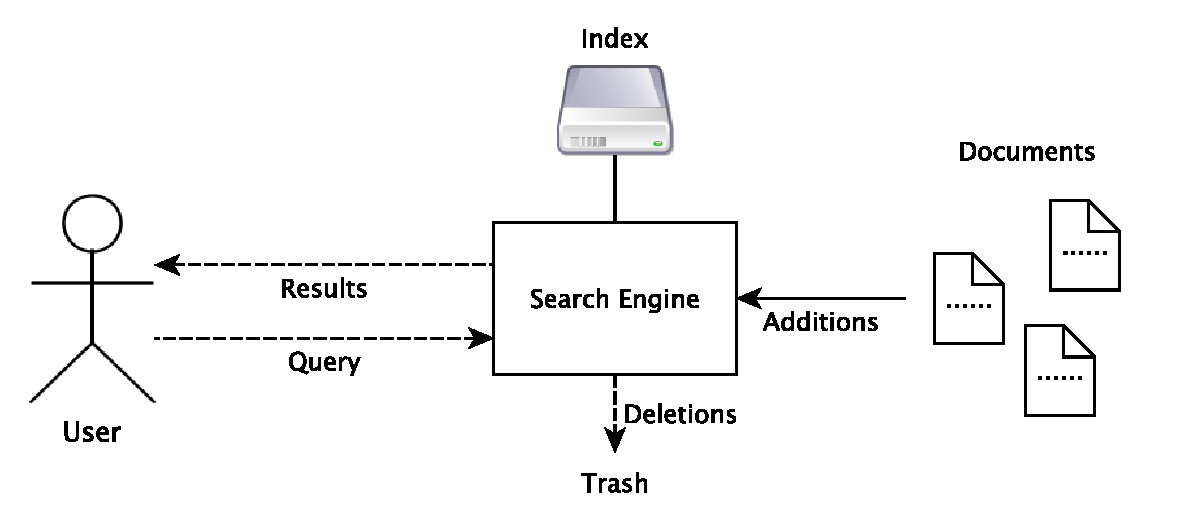
\includegraphics[scale=1]{pics/IR}
}%
\caption{Principal components of an IR system.}
\label{fig:IR}
\end{figure}
}
\label{chap:IR}
\section{Inverted Index}
\label{sec:inverted-index}

An index can be seen as a matrix with the terms (e.g. unigram) for rows and the
collection's documents as columns. In this matrix, an element
equal to one if the term i occurs in document j, and zero if not. However such
a matrix contains practically only zeros, thus a lot of wasted space. Inverted
List is a basic IR structure that reduces such a matrix to only store ones'
values. All the inverted lists taken together form the inverted index.

From the collection a dictionary of the words appearing in is created. The
dictionary's terms have been first filtered, by removing the punctuation for
example. Given a term from the dictionary, a linked list is associated to it
and stores all documents records where the term occurs in. A document record
can be simply a serial number of the document (i.e., document identifier), but
additional information like the term frequency and the position can be given.
The term frequency corresponds to the number of occurrences of the term in a
document, and the position indicate the positions of the occurrences within
that document. The Figure~\ref{fig:inverted-list} depicts two inverted lists
storing documents identifiers as integers, term frequencies and positions.
These inverted lists are built using the terms ``killed'' and ``brutus'' from
documents in the Table~\ref{tab:indexing}. There
is a relation one-to-one between documents identifiers and term frequencies,
and a relation many-to-many with the positions. There are as much position
values as there are occurrences (i.e., term frequency) of the term in the
document. The documents identifiers are stored in increasing order in order
to process queries, as presented in Section~\ref{sec:query-model}.

\begin{figure}
\centering
\resizebox{0.8\linewidth}{!}{%
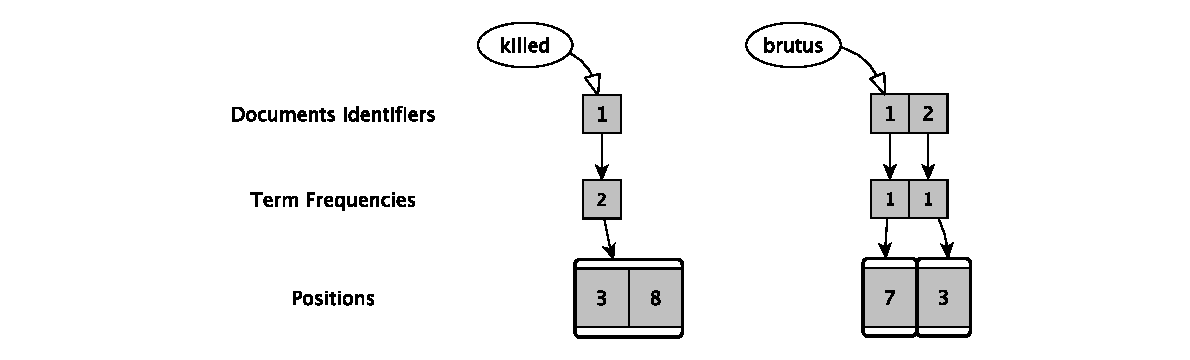
\includegraphics[scale=1]{pics/inverted-list}
}%
\caption{Inverted lists for the terms ``killed'' and ``brutus'' in documents
from the Table~\ref{tab:indexing}. Each inverted list stores the documents
identifiers, the term frequencies and the positions information.}
\label{fig:inverted-list}
\end{figure}

\subsection{Indexing}
\label{sec:IR-indexing}

In this section, traditional inverted index construction is presented, then the
block-based construction which makes possible to handle large collection.
Finally I discuss the importance of compression for large collection, and
present a commonly used  in Information Retrieval encoding technique.

An inverted index is the group of inverted lists built from a collection.
The basic steps to create an inverted index in the main memory from a collection
of documents are:
\begin{enumerate}
  \item make a first pass through the collection to gather term-document-i~dentifiers pairs
  \item sort the pairs with the term value as the key
  \item group together docIDs of a same term into an inverted list.
\end{enumerate}
These steps are reported in Table~\ref{tab:indexing} with two documents taken
from the ``Shakespeare's Collected Works'', storing only the document
identifier (docID) in the inverted lists and the document frequency (DF), i.e.
the number of documents the term appears in. Each words in the documents are
filtered by removing the punctuation and lowering the case. The set of terms
defines the dictionary of the inverted index. For each of the dictionary, an
inverted list is then created.

In order to build an inverted index once and for all, the in-memory
inverted index is written to the disk into what is called an \emph{inverted
file}. The Figure~\ref{fig:indexing} summarize the steps from the
collection to the creation of an inverted file. The inverted file contains all
the inverted lists, written one after the other. The dictionary is also stored
in that same file, where each term possess information about the inverted list
it points to: the inverted list's offset or the document frequency, i.e., the
number of documents the term appears in.

\begin{table}
\resizebox{\linewidth}{!}{%
\begin{tabular}{lrllrlllcl}
\toprule
\multicolumn{5}{l}{
{\bfseries Document 1:}
I was killed i' the Capitol; Brutus killed me.
}&
\multicolumn{5}{l}{
{\bfseries Document 2:}
The noble Brutus hath told you Caesar was ambitious.
}\\
\multicolumn{10}{c}{\phantom{a}}\\
{\bfseries term} & {\bfseries docID} & & {\bfseries term (sorted)} & {\bfseries
docID} & & {\bfseries term} & {\bfseries DF} & & {\bfseries Inverted List}\\
I & 1 & \multirow{18}{*}{$\Longrightarrow$} & ambitious & 2 &
\multirow{18}{*}{$\Longrightarrow$} & ambitious & 1 & $\mapsto$ & $1$ \\
was & 1 & & brutus & 1 & & brutus & 2 & $\mapsto$ & $1 \rightarrow 2$ \\
killed & 1 & & brutus & 2 & & capitol & 1 & $\mapsto$ & $1$ \\
i' & 1 & & capitol & 1 & & caesar & 1 & $\mapsto$ & $1$ \\
the & 1 & & caesar & 2 & & hath & 1 & $\mapsto$ & $1$ \\
capitol & 1 & & hath & 2 & & I & 1 & $\mapsto$ & 1 \\
brutus & 1 & & I & 1 & & i' & 1 & $\mapsto$ & $1$ \\
killed & 1 & & i' & 1 & & killed & 1 & $\mapsto$ & $1$ \\
me & 1 & & killed & 1 & & me & 1 & $\mapsto$ & $1$ \\
the & 2 & & killed & 1 & & noble & 1 & $\mapsto$ & $1$ \\
noble & 2 & & me & 1 & & the & 2 & $\mapsto$ & $1\rightarrow 2$ \\
brutus & 2 & & noble & 2 & & told & 1 & $\mapsto$ & $1$ \\
hath & 2 & & the & 1 & & you & 1 & $\mapsto$ & $1$ \\
told & 2 & & the & 2 & & was & 2 & $\mapsto$ & $1 \rightarrow 2$ \\
you & 2 & & told & 2 & & & & \\
caesar & 2 & &  you & 2 & & & & \\
was & 2 & & was & 1 & & & & \\
ambitious & 2 & & was & 2 & & & & \\
\bottomrule
\end{tabular}
}%
\caption{Inverted index creation from two documents taken in ``Shakespeare's
Collected Works''. Each word is filtered and associated to its document
identifier (docID). After sorting the pairs on the term, the inverted lists are
created for the set of terms. The inverted lists store only the docID of the
document the term appears in.}
\label{tab:indexing}
\end{table}

\begin{figure}
\centering
\resizebox{0.8\linewidth}{!}{%
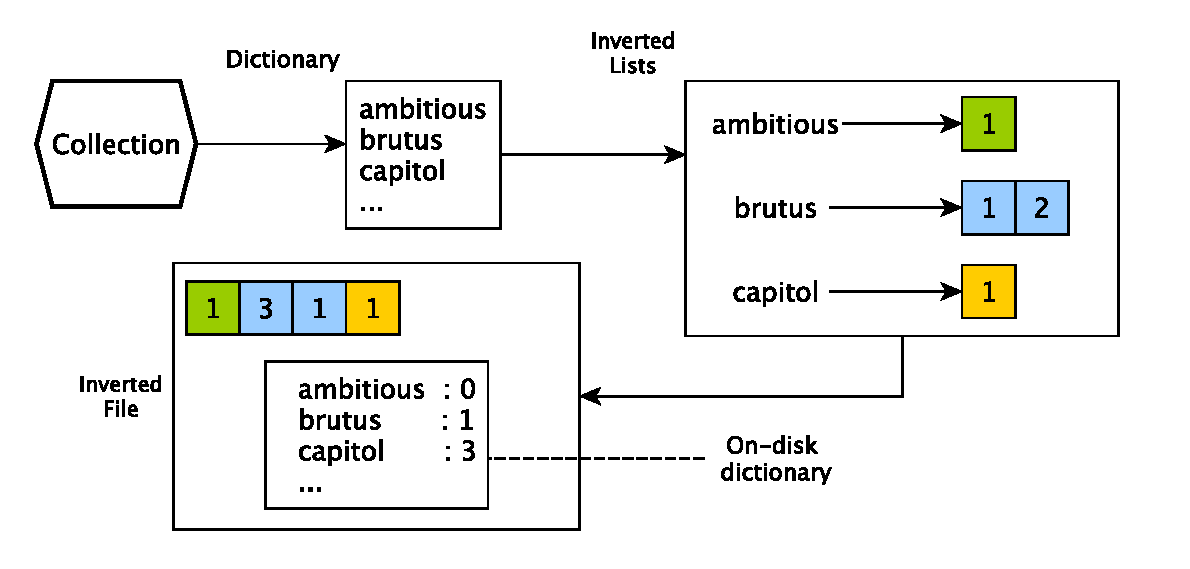
\includegraphics[scale=1]{pics/indexing}
}%
\caption{Indexing, from a collection of documents to the inverted file. The
in-memory inverted lists are written to disk one after the other. The
terms of the embedded dictionary possess offset to the associated inverted list
in the file.}
\label{fig:indexing}
\end{figure}

\subsubsection{Merge-Based Indexing}

The previous indexing technique works in-memory, and then cannot handle large
collection with large inverted lists. Merge-based indexing is a technique that
divides an inverted index construction into segments, which are then merged
together to form a complete inverted index. Thus an inverted list can span
over multiple segments. When the main memory is filled or that a threshold has
been reached, a segment is written to a secondary storage space (e.g. the disk)
into an inverted file. Each on-disk inverted file contains an inverted index
independent from the one in an other segment. When merging inverted files, it is
then necessary to update inverted lists of a same term but stored in different
segments. The Figure~\ref{fig:merged-indexing} depicts the merge process of
three inverted files into one. An inverted list spans over these files: the
documents identifiers values are then local to each file. Thus it is necessary
to update these identifiers numbers in order to keep an ordered inverted list
after merging.

Such an index construction requires two steps to finish. The first one consists
in building multiple segments and is called the \emph{commit} step. The second
one consists in the merging process of multiple files into one inverted file
and is called the \emph{optimization} step. These steps are believed to
be a common operation for incremental inverted index.

\begin{figure}
\centering
\resizebox{0.8\linewidth}{!}{%
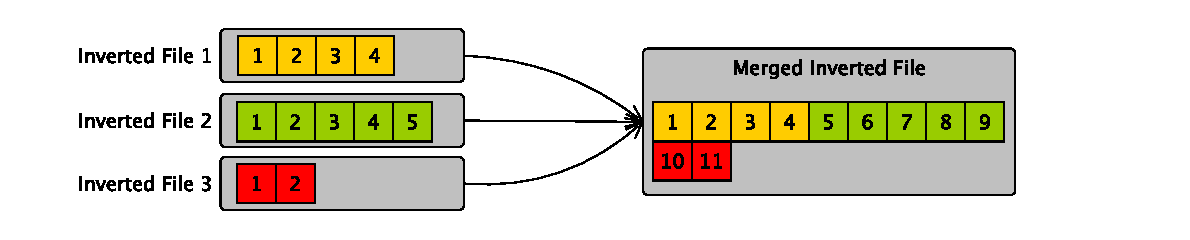
\includegraphics[scale=1]{pics/merged-indexing}
}%
\caption{Merge-based indexing of three inverted files. An inverted list, storing
documents identifiers, spans over these files. When merging these files into
one inverted file, the documents identifiers are updated to keep an ordered
list.}
\label{fig:merged-indexing}
\end{figure}

\subsubsection{Block-Based Inverted List}
\label{sec:compression:block}

For performance and compression efficiency, it is best to store separately each
data stream of an inverted list~\cite{anh:2006:siohttq}. In a non-interleaved
index organisation, the inverted index is composed of three inverted files,
one for each stream of values (i.e., documents identifiers, frequencies and
positions). Each inverted file stores contiguously one type of list, and three
pointers are associated to each term in the lexicon, one pointer to the
beginning of the list in each inverted file.

An inverted file is partitioned into blocks, each block containing a fixed
number of integers as shown in Figure~\ref{fig:index-structure}. Blocks are
the basic units for writing data to and fetching data from disk, but also the
basic data unit that will be compressed and decompressed. A block starts with
a block header. The block header is composed of the length of the block in
bytes and additional meta-data information that is specific to the compression
technique used. Long inverted lists are often stored across multiple blocks,
starting somewhere in one block and ending somewhere in another block, while
multiple small lists are often stored into a single block. For example, 16
inverted lists of 64 integers can be stored in a block of 1024 integers.

\begin{figure}
  \centering
	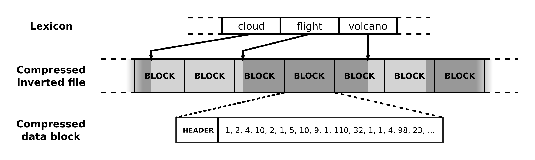
\includegraphics[scale=1.2]{pics/index-structure}
	\caption{Inverted index structure. Each lexicon entry (term) contains a
	pointer to the beginning of its inverted list in the compressed inverted
	file. An inverted file is divided into blocks of equal size, each block
	containing the same number of values.}
	\label{fig:index-structure}
\end{figure}

\subsubsection{Index Updates Strategies}

Updating the inverted index with new documents is done via two approaches: by
\emph{batches} or \emph{incrementally}.
The update strategy by batches stores
added documents into a buffer, and writes them to the index on-disk when some
threshold is reached. While this is adapted to static indexes, in other words
indexes that do not need to be updated right away. However in some cases such
as Internet news search engines, the user would expect the index to be updated
as soon new documents are detected. This use case is matched by incremental
updates strategy. With this strategy, the index is composed of the ones on
disk, but also with an index built in-memory. This second index holds the
updated documents temporarily that are bound to be written to the index on-disk
when a threshold is reached.
The question of deleted documents is handled thanks to a table that stores the
documents flagged in deleted state.

\subsection{Delta-Encoding}

Large collections result in large inverted files. As these files are stored on
disk, compressing their data is then crucial in order to save storage space.
\emph{Delta-encoding} is a basic encoding commonly used in Information
Retrieval which aims to decrease the size of inverted lists, thus reducing
inverted files disk space.

With an ordered and increasing list of integers, it is possible to considerably
reduce the size by storing not the actual integers values but the gaps. A gap
is the difference between two consecutive integers. As the list is increasing,
the difference between an integer at position $i$ and an integer at position
$i-1$ will always be positive. To decompress a value at position i from a
delta-compressed list, we just have to sum up every values up to i. The
Figure~\ref{fig:delta-encoding} depicts a delta-compressed list of integers. By
storing gaps values, we can reduce the size of the list from 88 to 38 bits.

Documents identifiers are stored in increasing order in each inverted list, and
can then be delta-encoded. Also the positions values are stored in increasing
order, but they are local to a document. Thus position values relative to a
same document are delta-encoded, and the encoding is re-initialized when
changing documents.

\begin{figure}
\centering
\resizebox{0.8\linewidth}{!}{%
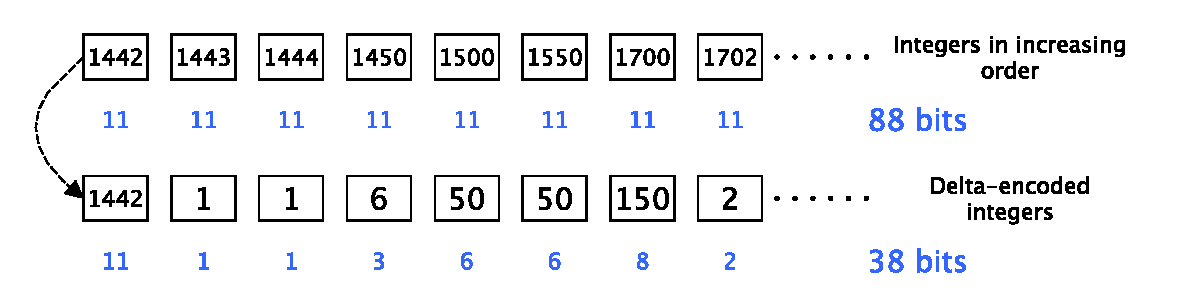
\includegraphics[scale=1]{pics/delta-encoding}
}%
\caption{Delta-encoding of an increasing ordered list of integers, showing the
size in bits of the two lists.}
\label{fig:delta-encoding}
\end{figure}

\section{Query Model}
\label{sec:query-model}

A query is an user request for information about the collection. Documents
matching that query are returned back to the user. In this section, I present
the query model used in Information Retrieval and explain how keyword and
Phrase queries are processed.

The model used to represent documents is the \emph{vector space model},
commonly called the ``bag of words'' model. In this model documents and
queries are seen as vectors, where a component represent a term in the
collection. Given a query and a set of document vectors, we compute the angle
between them. The smaller this angle is, the higher the document will be
ranked with regards to the query.

The query model is a Boolean model, where terms that are to appear in the
returned documents are combined together using Boolean operators. Boolean
operators include two binary operators, i.e., \emph{AND} and \emph{OR}, and one
unary operator \emph{NOT}. Their operands can be either a term or a Boolean
sequence of terms. With this model, documents in the indexed collection are
nothing more than a set of terms. Set theory operations are used to interpret
such queries. The Boolean operators are binary operations and their operands are
set of words. The And operator is interpreted as an \emph{Conjunction},
the OR operator as an \emph{Disjunction} and the NOT operator as the
\emph{Exclusion}. A simple Boolean query on the two documents from the
Table~\ref{tab:indexing}
\begin{center}
brutus \emph{AND} ambitious
\end{center}
searches for all documents containing the terms brutus and ambitious.

In this model, a document is seen as a \emph{bag of words}, where the exact
ordering of terms is ignored but the number of occurrences of each term (i.e.
term frequency) is material.

\subsection{Keyword Query Processing}

Keyword queries search for documents containing the terms in the Boolean
expression. Their processing follows the algorithm
\begin{enumerate}
  \item Retrieve inverted lists of all the query's terms.
  \item Apply set operations, i.e., union, intersection or set difference, on the
  inverted lists.
  \item Returns documents mapping to the documents identifiers in the inverted
  list, resulting of the set operations.
\end{enumerate}
The former query ``brutus AND ambitious'' returns the document identifier 1, as
the intersection of their inverted list give only this one identifier. The
Figure~\ref{fig:KWquery} depicts the processing of that query, showing in red
the documents identifiers occurring in both inverted lists.

\begin{figure}
\centering
\resizebox{0.35\linewidth}{!}{%
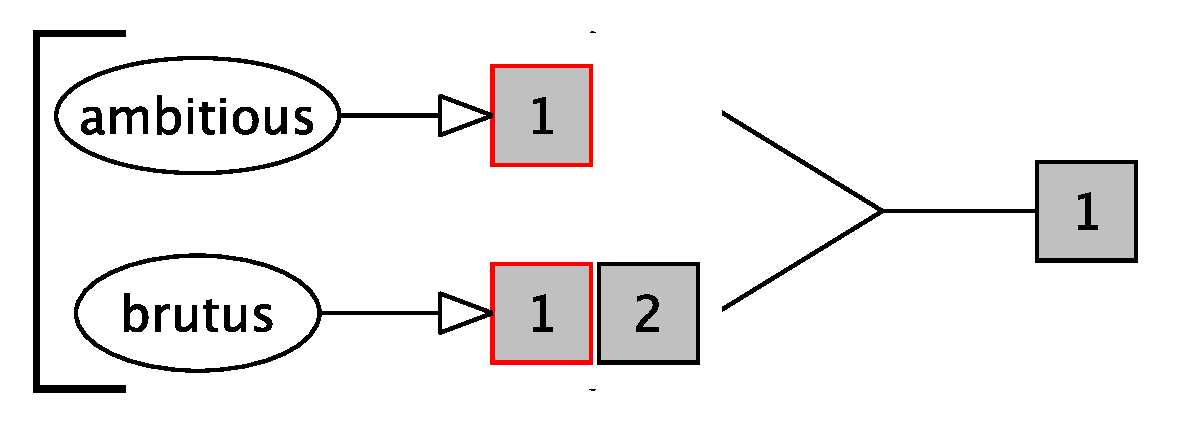
\includegraphics[scale=1]{pics/KWquery-processing}
}%
\caption{Processing of the keyword query ``brutus AND ambitious''. The only
document containing both terms is the document 1, from the
Table~\ref{tab:indexing}.}
\label{fig:KWquery}
\end{figure}

\subsection{Phrase Query Processing}

The position of terms in a document is very important, as it can change the
meaning of these terms in the document. For example the keyword query
``\emph{stanford AND university}'' may return a document containing the
sentence ``The inventor Stanford Ovshinsky never went to university''. However
the given query suggested to search information about a University in
Stanford. The returned document is then irrelevant to the query, to what really
is needed by the user. In order to perform more precise search, the position
information about the terms in documents is necessary. Indeed restricting the
search to documents having the keyword terms appear consecutively one after the
other will discard irrelevant documents. As four terms are between Stanford
and University in the former example, such a document will not be returned if
restricting to zero words in-between. The query that takes into account the
position of terms within documents are called \emph{Phrase queries}.

A \emph{n-gram} is a sub-sequence of n terms in the document. For instance, a
bi-gram (i.e., a sub-sequence of two terms) in document 1 in
Table~\ref{tab:indexing} can be ``I was'' or ``Brutus killed''. There exist
two ways to handle phrase queries. The first one relies on indexing n-gram
occurring in the collection. Indexing bi-gram would follow the same process as
in the Table~\ref{tab:indexing}, but with bi-gram instead of single terms.
However it restricts to bi-gram only, and to search for tri-gram (i.e., three
terms in the sub-sequence) it would mean to index also tri-gram. This is highly
inefficient as a huge storage space is then needed. The second way uses the
position information of terms within documents to process phrase queries. Thus
only uni-gram (i.e., one term in the sub-sequence) are indexed with the relative
position of each term. Also we can handle this way phrase queries with any
number of terms in the sub-sequence.

\subsubsection{Phrase queries processing algorithm}

The first step in processing phrase queries is the same as processing
keyword queries: after retrieving inverted lists of each term, we perform
operations on the inverted lists to get the list of documents identifiers
matching the terms in the query. The second step consists in filtering these
documents according to the position information. The algorithm to discard or
not a document works on the positions of keywords occurring in a same document,
and is as follows:
\begin{enumerate}
  \item[] Let R be the list of documents identifiers that results from the
  first step.
  \item For each document i in R.
  \item Retrieve the list $P_{T1,i}$ of positions for the term T1 in document i,
  and the list $P_{T2,i}$ of positions for the term T2 in document i.
  \item Compare position values $p_1 \in P_{T1,i}$ and $p_2 \in P_{T2,i}$
  \begin{enumerate}
    \item The absolute difference between $p_1$ and $p_2$ is \emph{greater than}
    1 $\Rightarrow$ within the list with the lower value, we advance until
    reading a position greater than the other value.
    \item The absolute difference between $p_1$ and $p_2$ is \emph{equal to} 1
    $\Rightarrow$ the current document is kept and we go to the next document
    in R.
  \end{enumerate}
\end{enumerate}
The Figure~\ref{fig:PQquery} depicts with dashed lines the comparisons performed
in the step 3 in the former algorithm. We first compare 1 and 8 and keep on
reading values in P1 until the value 20. Then the comparison between 20 and 8,
and so on. The algorithm stops at comparison 5, as the difference is equal to
1. The document is thus kept in the results of the phrase query. In the
Table~\ref{tab:indexing}, the phrase query ``brutus killed'' would match the
document 1, as the terms appear respectively in positions 7 and 8. We can note
that as the difference computed in steps 3 is absolute, the phrase query
``killed brutus'' also matches that document. This reflects the ``bag of
words'' query model in Information Retrieval.

\begin{figure}
\centering
\resizebox{0.9\linewidth}{!}{%
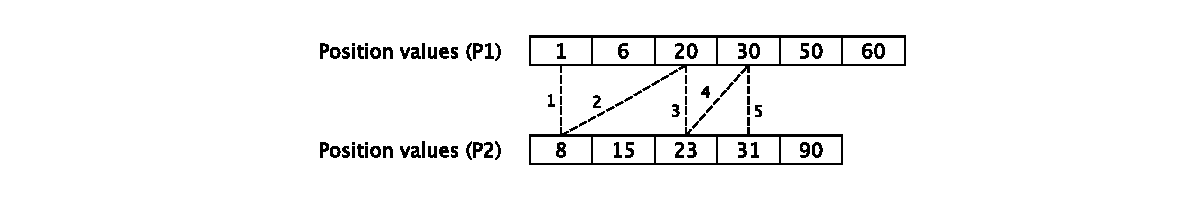
\includegraphics[scale=1]{pics/PQsearch}
}%
\caption{Documents filtering based on the position of terms. P1 and P2 are two
positions lists of two different terms occurring in the same document. Dashed
lines represent comparison between position values. The order in which these
comparisons are made is indicate by their label number.}
\label{fig:PQquery}
\end{figure}


\chapter{Semantic Web}{
The World Wide Web has drastically changed over the past decade. Tim
Berners-Lee is the person who introduced the idea of linked information thanks
to HyperText Markup Language (HTTP), which is the core of the web. The
expectations Tim Berners-Lee had of a global information space, where any data
can be read, written and shared is now concrete. The challenge is now to
organize this massive amount of knowledge and to improve the interactions
people have with this huge and complex system.

A major problem of the web comes directly from its core, the HTML. Thanks to
HTML, documents can be linked together, and a human can move from one document
to an other with those links. A computer is able to interpret this language,
however the content of documents is written in natural language, and is then
only accessible to people.

Most of the content on the web is only readable by people. One can read the
information of documents and understand its meaning. On the opposite, computers
only know to which documents a document is related to thanks to HTML markups.
However they do not carry descriptions about the content of a document and how
two documents are related to each other.

This is the reason why Internet applications like search engines have limited
capabilities. A search engine looks for a term T in a document, but it cannot
search for related documents, as it lacks a formal description of the content.
A search engine help people look for data, but in the end to find precise
information, he has to himself follow HTML links. This is a highly consuming
task, with limited results.

A solution is to provide computers with comprehensible Web data is to describe
documents and their relationships with meaningful metadata. The Semantic
Web aims to merge web resources with machine-understandable data to enable
people and computers to work in cooperation and to simplify the sharing and
handling of large quantities of information.

In this chapter I present the vision of the Semantic Web, before describing the
various technologies in the Semantic Web. Then I present how Web data is
represented to make it machine-understandable. Finally I present some projects
that use Semantic Web technologies.
}
%%%%%%%%%%%%%%%%%%%%%%%%%%%%%%%%%%%%%%%%%%%%%%%%%%%%%%%%%%%%%%%%%%%%%%%%%%%%%%
\label{chap:SW}
\section{The Framework}

The Semantic Web defines a set of technologies which are a standard on how to
describe, manipulate and query Semantic data to have in the end a solid base of
machine-readable knowledge. The Semantic Web presents a layer hierarchy
(Figure~\ref{fig:sw-stack}), where each layer has its own purpose. A layer of
this Semantic Web Stack uses the information provided by layers below. This
shows how Semantic Web is made possible and how it is not a replacement of the
current Web but an extension.

\begin{figure}
\centering
\resizebox{0.5\linewidth}{!}{%
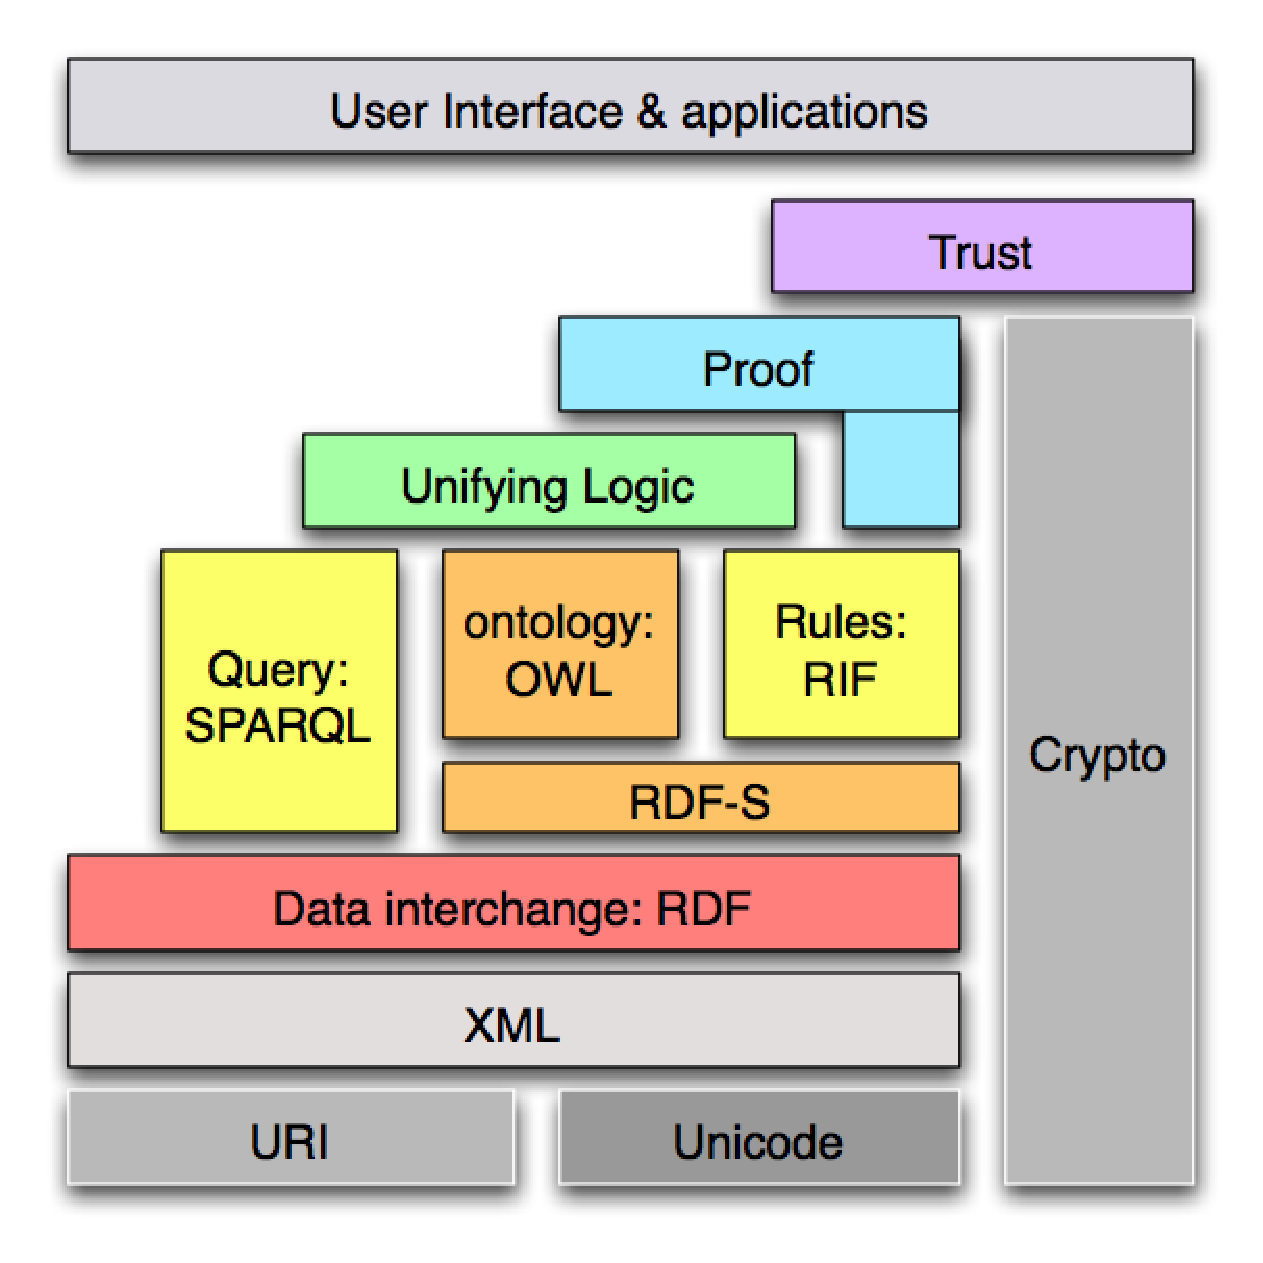
\includegraphics[scale=1]{pics/SemWebStack}
}%
\caption{The Semantic Web Stack. It presents each layer of the Semantic Web,
where each have a defined a purpose and that make the Semantic extension of the
Web as we know it possible.}
\label{fig:sw-stack}
\end{figure}

\begin{description}
\item[Uniform Resource Identifier (URI)] provides means for uniquely
identifying semantic web resources.
\item[Unicode\footnote{\url{http://www.unicode.org/standard/versions/}}] 
serves to represent and manipulate text in many languages. Semantic Web should
also help to bridge documents in different human languages, so it should be
able to represent them.
\item[XML] extensible Markup Language (XML) is the standard syntax that
enables creation of documents composed of structured data. Semantic web gives
meaning (semantics) to structured data. 
\item[Resource Description Framework (RDF)] is the standardized representation
of meta-data.
\item[RDF Schema (RDFS)] provides basic vocabulary for RDF.
\item[Web Ontology Language (OWL)] extends RDFS and allows a more complex
representation of resources (i.e., ontology). It gives then the possibility of
more advanced reasoning over data.
\item[SPARQL] is a RDF query language. It can be used to query any RDF-based
data and provide information to Semantic Web applications.
\item[Logic-Proof] a reasoning layer that infers new knowledge from the data.
\item[Trust] prove the trustfulness of the data thanks to cryptographic
techniques.
\item[User Interface] is the final layer that will enable humans to use
semantic web applications.
\end{description}

URI is a string that is used to identify resources over the Internet. It is
often used by markup languages to specify external documents or a specific
section of that document. For instance \emph{\url{http://di2.deri.ie/}} is an
URI that describes the Data Intensive Infrastructure unit.

An ontology in Information Science is a formal representation of knowledge as a
set of concepts within a domain, and the relationships between those concepts.
It is used to reason about the entities within that domain, and may be used to
describe the domain. For example we can have a simple ontology describing
animals like rats and cats are mammals; a mammal is an animal. Such an ontology
can be used when searching for terms in different domains.

\section{RDF: Resource Description Framework}

RDF is a framework that allows data on the web to be shared and reused across
applications. It provides features that facilitate data to be interchange
between datasets, even if they have different ontology.
RDF is used to describes things in the Internet, and the relations between
things. It extends the linking structure of the Web to use URIs to name the
relationship between concepts or objects as well as the two ends of the link.
This linking structure of the Web forms a directed, labeled graph called
\emph{RDF graph}, where the edges represent the relationship between two
objects, the graph nodes.

\subsection{RDF Model}

RDF is a standard
model\footnote{\url{http://www.w3.org/TR/2004/REC-rdf-concepts-20040210/\#section-Concepts}}
for data interchange on the Web. Two connected nodes and the named relation
form a \emph{triple}. The set of triples form the RDF graph. The three parts
that compose a triple are:
\begin{enumerate}
  \item a \emph{subject}: the resource that this triple describes.
  \item an \emph{object}: the resource that the subject is related to.
  \item a \emph{predicate}: the description of the link between the subject and
  the object.
\end{enumerate}
The Figure~\ref{fig:rdf-triple} depicts a triple as a node-arc-node
link. The direction of the arc is significant: it always points toward the
object. The nodes of an RDF graph are its subjects and objects. The meaning
given to a RDF graph is the conjunction of all its triples.

A RDF graph defines three types of nodes:
\begin{description}
\item[Literal] a literal is a simple string, used to describe dates, titles or
any text in natural language. A literal may be \emph{plain} or \emph{typed}:
	\begin{itemize}
	  \item A plain literal is a string combined with an optional language tag.
	  \item A typed literal is a string combined with a datatype URI.
	\end{itemize}
\item[URI reference (URIref)] a URIref is a Unicode string used in a RDF graph
to represent URIs, and it can have an optional fragment identifier which is
indicated by the character ``\#''. For example the URI reference
\url{http://www.w3.org/2000/01/rdf-schema#comment} shows the URI before \#, and
the fragment ``comment'' that indicates which identifier to use within the URI.
This particular fragment ``comment'' is used to describe the subject resource.
\item[Blank Node] a blank node refers to resources that are not identified.
\end{description}
In a triple, the subject can be either a URIref or a blank node. The predicate
must be a URIref, while the object can be either one of the three node types.

The URI tends to be very long, which becomes inconvenient when using frequently
a same URIref. QName is a name space used as an abbreviation of a URIref. Its
syntax is \emph{URI:fragment}. For example the fragment ``comment'' within the
URI \url{http://www.w3.org/2000/01/rdf-schema#} can be shortened to
\emph{rdfs:comment}, where rdfs is mapped to the URI.

In the drawing convention of a RDF graph, URIrefs and blank nodes are drawn with an
ellipse, and literals with a rectangle. The Figure~\ref{fig:rdf-graph} depicts
a RDF graph describing the work ``The Lord of the Rings'' written by J.R.R
Tolkien. In this graph, the QNames ``dbpprop'' and ``dbpedia-owl'' map
respectively to \emph{\url{http://dbpedia.org/property/}} and
\emph{\url{http://dbpedia.org/ontology/}}. This graph provides three different
triples describing the sequel. The RDF graph gives the meaning that the
resource \url{http://dbpedia.org/page/The_Lord_of_the_Rings} has for author
J.R.R Tolkien, that it was released in the years 1954-55 and that a portion of
the English abstract is ``The Lord of the Rings is an epic\ldots''. We also
know that an unknown resource preceding ``The Lord of the Rings" novel was also
written by Tolkien.

\begin{figure}
\resizebox{\linewidth}{!}{%
\subfloat[A triple]{%
\centering
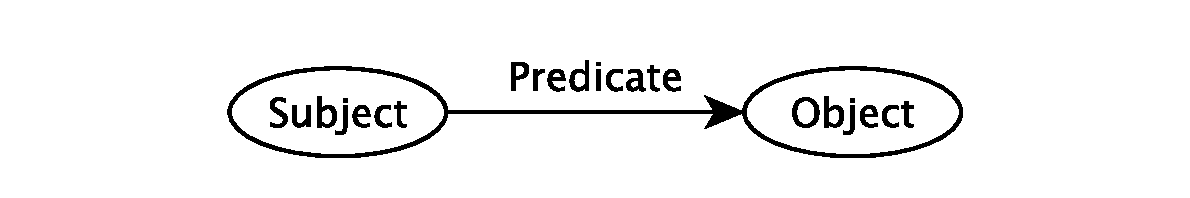
\includegraphics[scale=0.4]{pics/rdf-triple}
\label{fig:rdf-triple}
}\quad
\subfloat[A RDF graph describing the work ``The Lord of the Ring'' by J.R.R
Tolkien, using several QNames.]{%
\centering
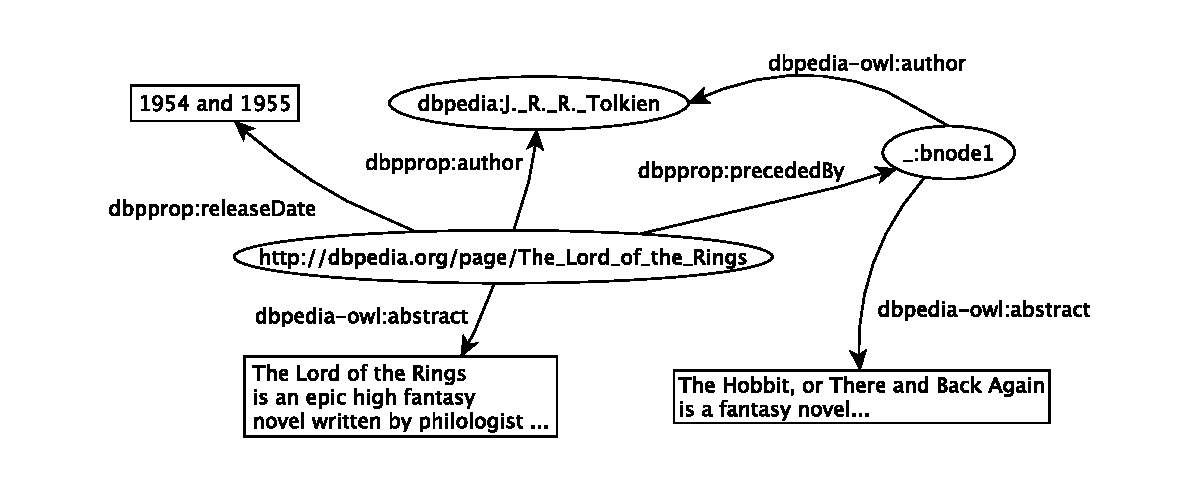
\includegraphics[scale=0.5]{pics/rdf-graph}
\label{fig:rdf-graph}
}}%
\caption{The RDF model used to represent knowledge.}
\end{figure}

\subsection{RDF Serialization}

Many serialization format for RDF have been developed, such as
RDFa\footnote{\url{http://www.w3.org/TR/xhtml-rdfa-primer/}} which is used to
embed RDF triples within XML documents. However during my internship only the
serialization format
\emph{N-Triple}\footnote{\url{http://www.w3.org/TR/rdf-testcases/\#ntriples}}
has been actively used, and so it will be the only one described here. Using
the N-Triple format, the triples within a RDF graph can be serialized with a
line-based plain text format. It is a format recommended to interchange data
between different applications.

This serialization uses an Extended Backus-Naur Form grammar, where each triple
is written into a line, ending with a point. The format is {\bfseries
\emph{Subject Predicate Object .}}\hs.
A URIref is written enclosed between the characters \emph{'$<$' '$>$'}. The
literals are written between double quotes, followed by an optional language
tag \emph{@language} for plain literals (e.g. ``bird"@en), and by
\emph{'\^{}\^{}'URIref} for typed literal (e.g.
``abc"\^{}\^{}$<$\url{http://example.org/datatype1}$>$, where abc is of type
datatype1). A blank node is represented by \emph{'\_':name}, where name is an
internal identifier which allows to have several blank nodes within a RDF
graph. The RDF graph in the Figure~\ref{fig:rdf-graph} can be serialized in
N-Triples format as in Table~\ref{tab:TL-ntriples} where \emph{TLR} refers to
the URI \url{http://dbpedia.org/page/The_Lord_of_the_Rings}.

\begin{table}
\centering
\resizebox{0.9\linewidth}{!}{%
\begin{tabular}{lclclcl}
$<$TLR$>$&\phantom{a}&$<$dbpprop:author$>$&\phantom{a}&$<$dbpedia:J.\_R.\_R.\_Tolkien$>$
&\phantom{a}&.\\
$<$TLR$>$&\phantom{a}&$<$dbpprop:releaseDate$>$&\phantom{a}&``1954 and
1955''&\phantom{a}&.\\
$<$TLR$>$&\phantom{a}&$<$dbpedia-owl:abstract$>$&\phantom{a}&``The Lord of
the Rings is an epic\ldots''&\phantom{a}&.\\
$<$TLR$>$&\phantom{a}&$<$dbpprop:precededBy$>$&\phantom{a}&$\_:bnode1$&\phantom{a}&.\\
$\_:bnode1$&\phantom{a}&$<$dbpedia-owl:author$>$&\phantom{a}&$<$dbpedia:J.\_R.\_R.\_Tolkien$>$&\phantom{a}&.\\
$\_:bnode1$&\phantom{a}&$<$dbpedia-owl:abstract$>$&\phantom{a}&''The Hobbit, or
There and Back Again is a fantasy novel\ldots''&\phantom{a}&.\\
\end{tabular}
}%
\caption{N-Triple representation of the RDF graph in
Figure~\ref{fig:rdf-graph}.}
\label{tab:TL-ntriples}
\end{table}

\subsection{SPARQL}

The RDF model introduce a mean to represent data and any type of data can,
at least to some degree, be represented in this model. SPARQL\footnote{SPARQL:
\url{http://www.w3.org/TR/rdf-sparql-query/}} is a standardized query language
for RDF. Designed so that queries can be expressed across diverse data, SPARQL
is able to express not only conjunction and disjunction of RDF graphs but also
complex queries, e.g. by using supplementary binary operators such as
arithmetic operators and comparisons in various filters.

A SPARQL query contains a set of \emph{triple patterns} that matches a
sub-graph of RDF graphs. Triple patterns are expressed in the same way as RDF
triples, i.e., subject, predicate, object, the difference being that any part of
that triple can be a variable. Typical SPARQL queries are graph patterns
combining SQL-like logical conditions over RDF statements with
regular-expression patterns. The result of a query is a set of sub-graphs
matching precisely the graph pattern defined in the query. For instance, the
SPARQL query
\begin{quote}
\begin{flushleft}
PREFIX dbpprop:    $<$http://dbpedia.org/property/$>$\\
SELECT ?abstract\\
WHERE\\
\{\\
\begin{quote}
$<$TLR$> \; <$dbpprop:author$> \;$ ?abstract $\;$ . 
\end{quote}
\}
\end{flushleft}
\end{quote}
has a single triple pattern that matches the first row of the triples in the
Table~\ref{tab:TL-ntriples}. The first line shows the QName used in the query.

% \subsection{Reasoning}
% 
% Reasoning is the cognitive process to look for conclusions and beliefs.
% Reasoning allows to create links between two objects that are somehow related
% but only implicity, granting thus the machine to enlarge its searching scope.
% For example, we know that a monkey is a mamal and that mammals are an animal
% species, but how can a machine deduces that a monkey is also an animal. Through
% reasoning over RDF graphs, it is possible to ``create'' more knowledge,
% \emph{implicit} knowledge, from the explicit relations already existing. For
% example, the RDFS schema possesses inheritance reasoning capabilities
% through the property \emph{subClassOf} such as
% \begin{quotation}
% (rdf:type Morris Cat)
% 
% (rdfs:subClassOf Cat Mammal),
% \end{quotation}
% which implies that Morris is also a sub-class of mammal.


%%%%%%%%%%%%%%%%%%%%%%%%%%%%%%%%%%%%%%%%%%%%%%%%%%%%%%%%%%%%%%%%%%%%%%%%%%%%%%
\chapter{SIREn}{
People are using more and more Semantic Web technologies and the quantity of
Semantic data will keep on expanding. Scalable and performant RDF management
systems are then becoming a necessity for semantic applications in order to use
thoroughly semantic data. Moreover traditional search engines do not use the
structured information available with semantic data. Taking the e-commerce as
an example, looking for a particular product is done by entering keyword
queries into the search engine and web pages are returned. However these
documents are most of the time irrelevant as they only include the key words,
but are not necessarily about the product itself. Also such web pages are
likely to provide information about other unrelated products as well. What is
really looked for then is the \emph{entity} of the product and anything that
can be related to that entity.

Sindice\footnote{Sindice: \url{http://sindice.com/}} is a web service which
purpose is to offer efficient searching capabilities over the semantic data.
Sindice is built on top of the Semantic Information Retrieval Engine,
SIREn\footnote{SIREn: \url{http://siren.sindice.com/}}, a system based on
Information Retrieval which goal is to search not for web pages but for
``entities''.

In this chapter, the indexing model of SIREn is presented before introducing
its query model.}
%%%%%%%%%%%%%%%%%%%%%%%%%%%%%%%%%%%%%%%%%%%%%%%%%%%%%%%%%%%%%%%%%%%%%%%%%%%%%%
\label{chap:BG-siren}
\section{Related Work}

In this section, we describe the current approaches for indexing RDF data,
before reviewing the existing search models for (semi) structured data.

\subsection{Retrieval of RDF Data}

The growth of RDF data incurs the need of efficient and scalable data
management systems. Several systems have been proposed based on Relational
DataBases Management Systems (RDBMS)~\cite{beckett:2003:swss-rdbms}. RDF data
management systems are able to store a large amount of data and use SPARQL as a
query language which allows to perform complex searches over the collection. A
user is able to perform complex request when the database schema is known.
However given the heterogeneous data collection on the web, the added value of
SPARQL is limited. Indeed it is difficult to write precise queries since the
data structure and the ontology may vary from one dataset to an other.

Other
approaches~\cite{guha:2003:tap,ding:2005:swoogle,harth:2008:swse,cheng:2008:falcons}
carried over keyword-based search to Semantic Web and RDF data in order to
provide ranked retrieval using content-based relevance estimation. In
addition, such systems are easier to scale due to the simplicity of their
indexing scheme. However, such systems are restricted to keyword search and do
not support structural constraints. These systems do not consider the rich
structure provided by RDF data.

A first step towards a more powerful search
interface combining imprecise keyword search with precise structural
constraints has been investigated by Semplore~\cite{wang:2009:semplore}.
Semplore has extended inverted index to encode RDF
graph approximations and to support keyword-based tree-shaped queries over RDF
graphs. However the increase of query capabilities comes at a cost, and the
scalability of the system becomes limited.

\subsection{Search Models for (semi) Structured Data}

In addition to standardised query languages such as SPARQL, a
large number of search models for semi-structured data have been developed. Some
of them focus on searching structured
databases~\cite{agrawal:2002:dbxplorer,bhalotia:2002:banks,hristidis:2002:discover,liu:2006:sigmod},
XML documents~\cite{cohen:2003:xsearch,guo:2003:xrank,liu:2007:xseek} or
graph-based data~\cite{abiteboul:1996:lorel,kachiola:2005:vldb,li:2008:ease}
using simple keyword search. Simple keyword-based search has the advantages of
\begin{inparaenum}[(1)]
\item being easy to use by users since it hides from the user any structural
information of the underlying data collection, and
\item of being applicable on any scenarios. 
\end{inparaenum}
On the other hand, the keyword-based approach suffers from limited capability
of expressing various degrees of structure when users have a partial knowledge
about the data structure.

Other
works~\cite{kasneci:2008:naga,mandreoli:2009:edbt,wang:2009:semplore,dong:2007:sigmod,fletcher:2009:theory-search}
have extended simple keyword-based search with structured queries
capabilities. \cite{dong:2007:sigmod,fletcher:2009:theory-search} propose a
partial solution to the lack of expressiveness of the keyword-based approach
by allowing search using conditions on attributes and values.
\cite{kasneci:2008:naga,mandreoli:2009:edbt,wang:2009:semplore} present more
powerful query language by adopting a graph-based model. However, the increase
of query expressiveness is tied with the processing complexity, and the
graph-based models
\cite{kasneci:2008:naga,mandreoli:2009:edbt,wang:2009:semplore} are not
applicable on a very large scale.

The search model introduced in Section~\ref{sec:siren-model} is similar to
\cite{dong:2007:sigmod,fletcher:2009:theory-search}, i.e., it is defined
around the concept of attribute-value pairs. However, our model is more
expressive since it differentiates between single and multi-valued attributes
and it considers the provenance of the information.

\section{Formal Model}
\label{sec:siren-model}

The expansion of Semantic Web applications has increased considerably and it
will continue on this progression. A wide range of different technologies has
been developed to represent and use semantic data. For the purpose of covering
a majority of data sources when searching for entities, a formal model has been
introduced. In this section, I give a summary of a labeled directed graph
model, before describing its query model.

\subsection{Entity Attribute-Value Model}

Semantic data can be used to describe any kind of data, from a physical person
to an abstract notion. These \emph{entities} are at the core of any data and
are the unit that is to be searched for with SIREn. This section presents
fundamentals about the Entity Attribute-Value model, a generic model which goal
is to support scenarios involving entities.

A Semantic graph (e.g. a RDF graph) is a graph that gives information about
several entities somehow related to each other. This graph can then be split
into sub-graphs, each one describing a particular entity. A \emph{star graph},
i.e., an entity at the center with associated incoming and outgoing relations.
For instance, the RDF graph in Figure~\ref{fig:rdf-graph} can be split into
three entities, as depicted in the Figure~\ref{fig:entities}. The graph
describing ``The Lord of the Rings'' work is divided into the
\emph{\url{http://dbpedia.org/page/The_Lord_of_the_Rings}}, \emph{\_:bnode1}
and \emph{dbpedia:J.\_R.\_R.\_Tolkien} entities.
% Also, the FOAF file from the
% Listing~\ref{lst:foaf} can be splitted into three entities: \emph{Giovanni
% Tummarello}, \emph{Renaud Delbru} and \emph{Stephane Campinas}.
The star graph gives information about the entity and is then generically
called an \emph{entity description}.

A \emph{dataset} is a source of semantic data, such as a domain or a site web
and it gives the \emph{context} of the data it contains. An \emph{attribute}
refers to the relation between an entity and an object, e.g. the predicate in
a RDF triple. For example ``dbpedia-owl:author'', ``dbpedia-owl:abstract'' and
``dbpprop:precededBy'' are the attributes associated with the \_:bnode1
entity. An attribute can also be \emph{multi-valued} as a book can have
multiple authors for instance. A \emph{value} refers to the node related to an
entity.

\begin{figure}
\centering
\resizebox{\linewidth}{!}{%
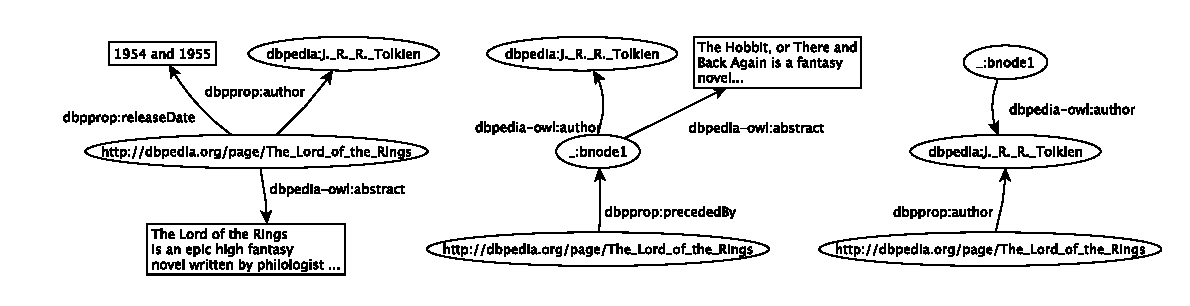
\includegraphics[scale=1]{pics/entities}
}%
\caption{A representation of the RDF graph in Figure~\ref{fig:rdf-graph}
divided into three entities: \emph{The Lord of the Rings}, \emph{\_:bnode1}
and \emph{Tolkien}.}
\label{fig:entities}
\end{figure}

\subsubsection{Node-Labelled Tree Model for RDF}

SIREn uses a node-labelled tree structure to capture the relationship between
values, attributes, entities and datasets. Taking the RDF data model (the
triple) as a support, the tree represent four kinds of nodes as depicted in the
Figure~\ref{fig:tree-model}:
\begin{itemize}
  \item the \emph{dataset} that indicates the context of the data.
  \item the \emph{entity} (the subject).
  \item the \emph{attribute} (the predicate).
  \item the \emph{value} (the object).
\end{itemize}
Each node can refer to one or more terms. In the case of RDF, a term is not
necessarily a word from a literal, but can be an URI or a local blank node
identifier.

A node-labelled tree model enables to encode and efficiently establish
relationships between the nodes of a tree. The two main types of relations are
Parent-Child and Ancestor-Descendant. To support these relations, the
requirement is to assign \emph{unique identifiers}, called node labels, that
encode the relationships between the nodes. The Dewey
encoding~\cite{beyer:2002:ordered-xml} is a simple node labelling scheme. In
Dewey Order encoding, each node is assigned a vector that represents the path
from the tree’s root to the node and each component of the path represents the
local order of an ancestor node. Using this labelling scheme, structural
relationships between elements can be determined efficiently. An element u is
an ancestor of an element v if label(u) is a prefix of label(v). The
Figure~\ref{fig:dewey-encoding} depicts the tree representation of the RDF
graph in Figure~\ref{fig:rdf-graph} using the Dewey encoding. The dataset is
the domain of the URI the graph is hosted at. In that representation, the
qualified names (i.e., QNames) have been removed in order to keep only the
property name, for clarity purpose since the property has the same semantic
even if the QNames are different (e.g., dbpprop:author and dbpedia-owl:author).
For example the entity ``The\_Lord\_of\_the\_Rings'' with vector [1.1], we can
find that it is a parent of the value node ``J.R.R.\_Tolkien'' with vector is
[1.1.2.1].

\begin{figure}
\centering
\subfloat[Conceptual representation of the node-labelled tree model.]{
\resizebox{0.34\linewidth}{!}{%
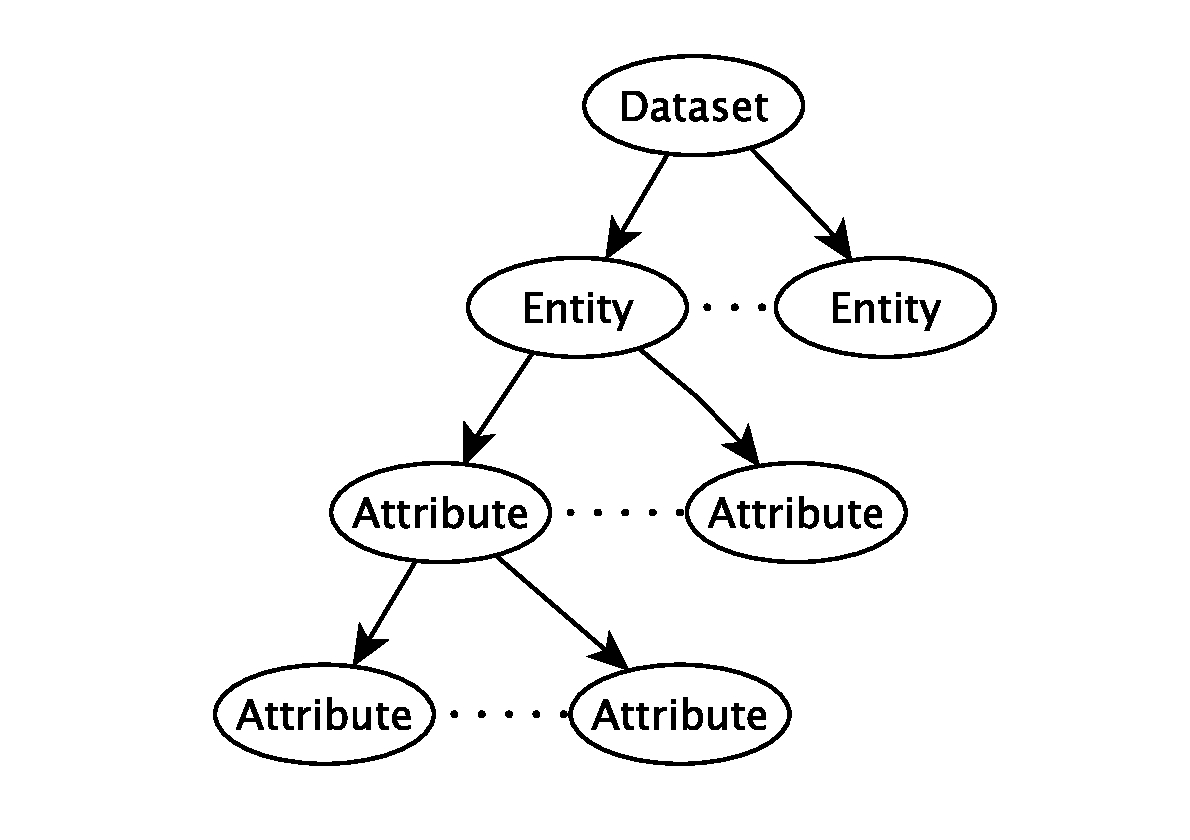
\includegraphics[scale=1]{pics/tree-model}
\label{fig:tree-model}
}}\quad
\subfloat[Node-labelled tree model with Dewey encoding of the dataset in
Figure~\ref{fig:rdf-graph}.]{
\resizebox{0.6\linewidth}{!}{%
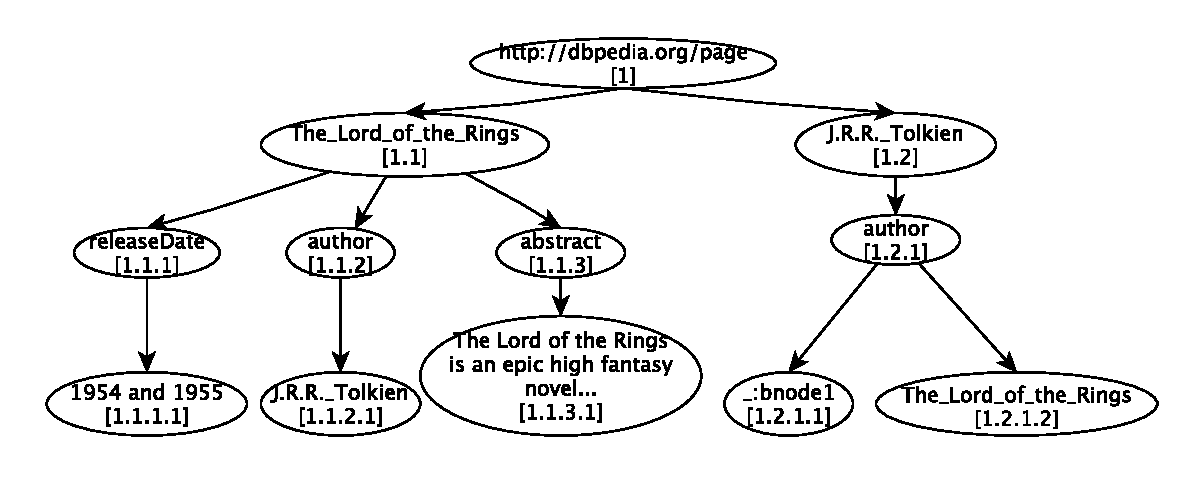
\includegraphics[scale=1]{pics/dewey-encoding}
\label{fig:dewey-encoding}
}}
\caption{The node-labelled tree model.}
\end{figure}

\subsection{Query Model}
\label{sec:siren-query-model}

Entities present a semi-structured structural view, and not a ``bag of
words'' as in traditional search engines. Therefore the query model search
entities with Boolean combinations of attribute-value pairs.

SIREn supports three different types of queries:
\begin{description}
\item[full-text:] traditional keyword query, useful when the schema of the
dataset is unknown;
\item[structural:] complex queries specified in a star-shaped structure, useful
when the data schema is known;
\item[semi-structural:] a combination of the two where full-text search can be
used on any part of the star-shaped query, useful when the data structure is partially known.
\end{description}
These query types provide different level of complexity, depending on the
knowledge of the data structure by the user. But the SIREn engine is aimed to
be used by other machines, and the possibility of complex queries are then
needed. The Figure~\ref{fig:star-query} depicts a star-shaped query that
matches the ``The Lord of the Rings'' entity from the
Figure~\ref{fig:entities}. This semi-structural query makes use of full-text
search through the use of keywords (e.g. ``tolkien'' or ``lord''). We can also
embedded Boolean search inside nodes, then the matching of entities having the
keywords ``lord'' and ``rings'' are marked as a positive match for the value
of an abstract (or label) attribute. The wildcard can also be used to describe
unknown relations between nodes. This search model is developed to find
entities that best match an entity description pattern (e.g. star-shaped
pattern).

In opposite to the full-text logical view where words are seen are seen as a
single bag of words, in the semi-structured view, the words are assigned to
multiple distinct bag of words, one for each value and attribute. Consequently,
it is possible to distinguish when words occur in a same value or different
values and avoid false-positive answers.

\begin{figure}
\centering
\resizebox{0.5\linewidth}{!}{%
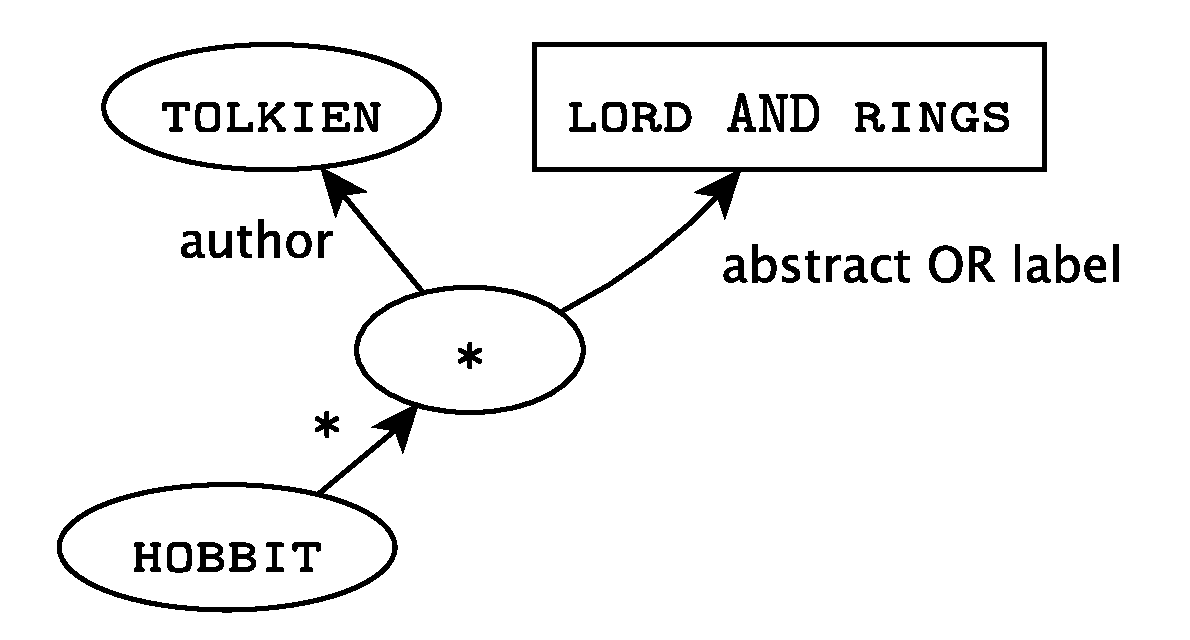
\includegraphics[scale=1]{pics/query}
}%
\caption{A star-shaped query matching the entity ``The Lord of the Rings''
from the Figure~\ref{fig:entities}. The character * stands for the wildcard
variable.}
\label{fig:star-query}
\end{figure}

\section{Model Implementation}

This section aims to present the implementation of the Entity Attribute-Value
model and of the query model over an inverted index. An overview of the
inverted index construction is presented with the entity-centric indexing
before describing more thoroughly the indexing structure.

\subsection{Entity-Centric Indexing}
\label{sec:ent-cent-indexing}

The search unit of the SIREn engine is an entity. As such,
SIREn aims to index entities (i.e., star graphs), and not documents
as the Section~\ref{sec:IR-indexing} presents it.
With a \emph{document-centric} indexing, every terms belong to a same document.
For instance the RDF graph in Figure~\ref{fig:rdf-graph} can be
taken as a whole document, since all data has been taken from the same web page
\url{http://dbpedia.org/page/The_Lord_of_the_Rings}. However when searching for
the entity \emph{The Lord of the Rings}, we just want information about this
entity and not also about any related work. This is a reason why SIREn uses an
\emph{entity-centric} indexing.

With a document-centric indexing, all the terms from the N-Triples of the
Figure~\ref{fig:rdf-graph} are seen as one document.
Then any queries on one of those terms will return that document. With an
entity-centric approach, we index the three different entities separately as
reported in the Table~\ref{tab:TLR-ent-cent}.

\begin{table}
\centering
\resizebox{\linewidth}{!}{%
\begin{tabular}{lc@{\hs}llll}
\toprule
Entity &\phantom{a}& \multicolumn{4}{c}{N-Triples}\\
\cmidrule{3-6}
% \multicolumn{6}{c}{\phantom{a}}\\
{\bfseries TLR} & \multicolumn{5}{c}{\phantom{a}} \\
\multirow{3}{*}{\phantom{a}}&\multirow{3}{*}{\phantom{a}}&
$<$TLR$>$&$<$dbpprop:author$>$&$<$dbpedia:J.\_R.\_R.\_Tolkien$>$&$.$\\
&&$<$TLR$>$&$<$dbpprop:releaseDate$>$&``1954 and 1955''&$.$\\
&&$<$TLR$>$&$<$dbpedia-owl:abstract$>$&``The Lord of the Rings is an
epic\ldots''&$.$\\

{\bfseries \_:bnode1} & \multicolumn{5}{c}{\phantom{a}} \\
\multirow{3}{*}{\phantom{a}}&\multirow{3}{*}{\phantom{a}}&
$<$TLR$>$&$<$dbpprop:precededBy$>$&\_:bnode1&$.$\\
&&\_:bnode1&$<$dbpedia-owl:author$>$&$<$dbpedia:J.\_R.\_R.\_Tolkien$>$&.\\
&&\_:bnode1 &$<$dbpedia-owl:abstract$>$&''The Hobbit, or There and Back
Again is a fantasy novel\ldots''&$.$\\

{\bfseries dbpedia:J.\_R.\_R.\_Tolkien} & \multicolumn{5}{c}{\phantom{a}} \\
\multirow{2}{*}{\phantom{a}}&\multirow{2}{*}{\phantom{a}}&
\_:bnode1&$<$dbpedia-owl:author$>$&$<$dbpedia:J.\_R.\_R.\_Tolkien$>$&.\\
&&$<$TLR$>$&$<$dbpprop:author$>$&$<$dbpedia:J.\_R.\_R.\_Tolkien$>$&.\\

\bottomrule
\end{tabular}
}%
\caption{Entity-centric indexing on ``The Lord of the Rings'' RDF graph of
Figure~\ref{fig:rdf-graph}. Each entity is reported with its star graph in the
N-Triples format.}
\label{tab:TLR-ent-cent}
\end{table}

SIREn stores triples documents into a table where each
documents are stored as rows, a column having a meaning for the
document (e.g. title, abstract, \ldots). The Table~\ref{tab:doc-centric}
reports a document-centric strategy for semantic data like RDF triples, where
the first column stores the triple's subject, the second one the predicate and
the third one the object. As an attribute can be multi-valued, a lot of space is
wasted as three rows are used to store three triples where only the object
changes. In order to save space, thus improving indexing and querying
performances since less data to be written and read, SIREn uses a
representation format called \emph{N-Tuples}. It consists to collapse all
triples with a same predicate into one row and to remove the subject cell, as
depicted in the Table~\ref{tab:ent-centric}.

\begin{table}
\centering
\resizebox{0.8\linewidth}{!}{%
\subfloat[Document-centric indexing.]{%
\begin{tabular}{ccc}
\toprule
$<$ s $>$ & $<$ p1 $>$ & $<$ o1 $>\;.$ \\
$<$ s $>$ & $<$ p1 $>$ & $<$ o2 $>\;.$ \\
$<$ s $>$ & $<$ p1 $>$ & $<$ o3 $>\;.$ \\
$<$ s $>$ & $<$ p2 $>$ & $<$ o4 $>\;.$ \\
\bottomrule
\end{tabular}
\label{tab:doc-centric}
}\quad%
\subfloat[Entity-centric indexing.]{%
\begin{tabular}{cccc}
\toprule
$<$ p1 $>$ & $<$ o1 $>$ & $<$ o2 $>$ &$<$ o3 $>\;.$ \\
$<$ p2 $>$ & $<$ o4 $>$ & $\;.$ & \\
\bottomrule
\end{tabular}
\label{tab:ent-centric}
}}
\caption{Two different indexing strategies for semantic data, e.g. RDF triples.
The characters ``s'', ``p'' and ``o'' refer respectively to the subject,
predicate and object in a triple.}
\end{table}

\subsection{Inverted Index Structure}
\label{sec:siren-inv-lists}

Traditionally in Information Retrieval-based search engines, there are three
streams of integers that form an inverted list. A stream of documents
identifiers, a stream of term frequencies and a stream of positions.
In SIREn there are five stream of integers, being streams of entity
identifiers, of term frequencies, of attributes identifiers, of values
identifiers and of positions, identifiers taken from the Dewey encoding
depicted in the Figure~\ref{fig:dewey-encoding}. The term frequency corresponds
to the number of the term's occurrences in an entity description (e.g. a star
graph). The term position corresponds to the relative position of the term
within its node.

Because of the Dewey encoding, the identifiers numerical values have a
clustering effect: the entity identifier is local to a dataset, and the
attribute identifier is local to that entity, and so on. The
Figure~\ref{fig:siren-inv-lists} depicts the five stream of identifiers that
together form the inverted list in SIREn.
As an example for the locality of identifiers values, the position 5 and 7 in
the entity 10 (i.e., blue squares) describe a same term in a same value node
(i.e., value node with identifier 3). However the green square is local to the
same attribute 5, but not to the same value node.

The repetitive structure of semantic data (e.g. a same URI in the predicate
cell) implies that combining the entity-centric indexing with a delta encoding
of the inverted lists result in a compact inverted index structure. Indeed
because of the locality of the values, the gap between integers will be small.

\begin{figure}
\centering
\resizebox{0.32\linewidth}{!}{%
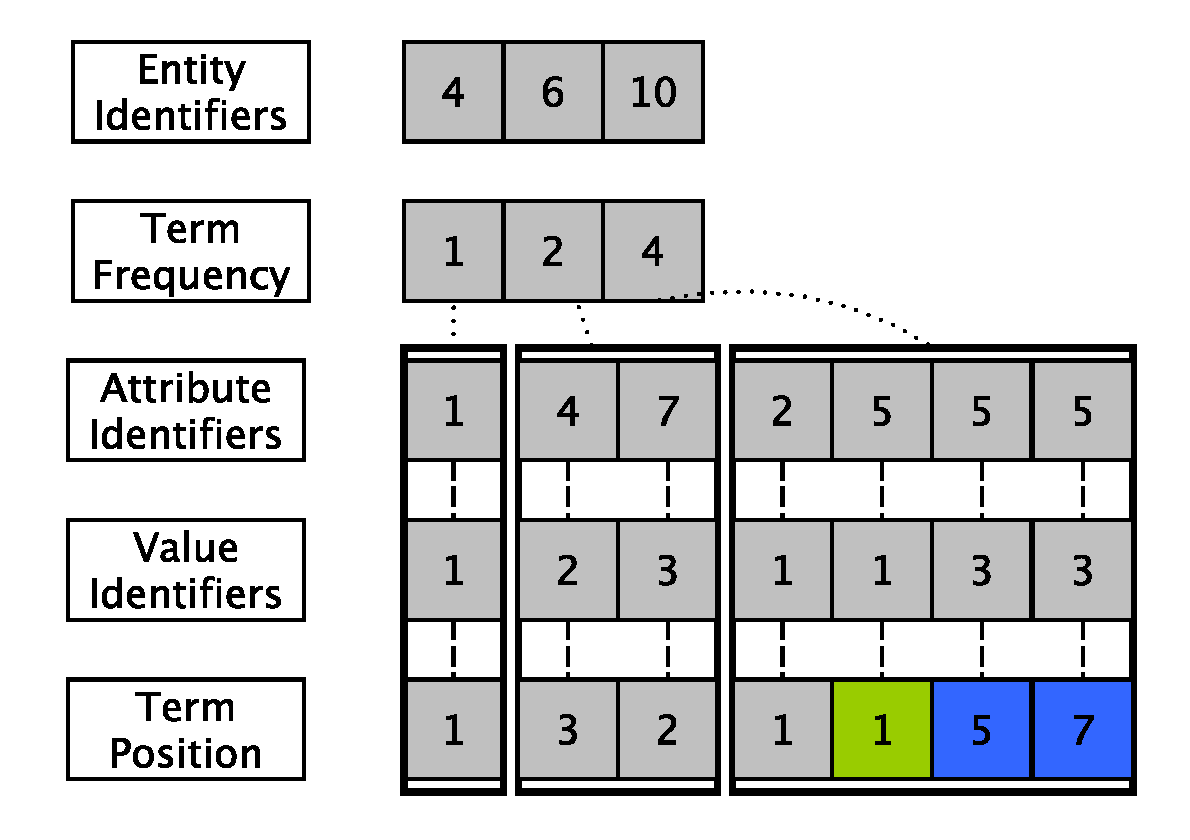
\includegraphics[scale=1]{pics/inverted-list-ex}
}%
\caption{Inverted Lists with the SIREn model.}
\label{fig:siren-inv-lists}
\end{figure}



%%%%%%%%%%%%%%%%%%%%%%%%%%%%%%%%%%%%%%%%%%%%%%%%%%%%%%%%%%%%%%%%%%%%%%%%%%%%%%
\chapter{Inverted List Compression}{
The inverted lists data, which are needed to process queries, are stored on
disk. This is the reason why reading the data is very costly on the queries
performance. The more data has to be read, and the slower the query response
will be. Thus inverted lists are compressed in order to reduce the number of
bytes read at query time, apart from the obvious goal to reduce disk space
consuming.

In this chapter, I present a state of the art of compression algorithms. While
Variable Byte is an algorithm that works on one integer at a time, Rice,
Simple family algorithms and Frame Of Reference-based techniques are
block-based. Given a block of integers from the list to compress, they aim to
compress it as best as possible using different approaches.}
%%%%%%%%%%%%%%%%%%%%%%%%%%%%%%%%%%%%%%%%%%%%%%%%%%%%%%%%%%%%%%%%%%%%%%%%%%%%%%
\label{chap:compression:state-of-the-art}
\section{Variable Byte}

Variable Byte (VByte) is an easy to implement algorithm, which makes it a
commonly used compression algorithm. VByte is a byte-aligned, i.e compression
at the byte level, algorithm that compress lists of values one integer at a
time. A compressed byte is divided in two parts
\begin{enumerate}
  \item the most significant bit is a \emph{flag} bit.
  \item the 7 bits left are used to store the integer.
\end{enumerate}
For an integer v to be compressed, the lower 7 bits are stored in one byte. The
flag is put at
\begin{inparaenum}[(a)]
\item 1 if there is still bits remaining in v or 
\item 0 otherwise.
\end{inparaenum}
This process is repeated until no more bits are left. The Table~\ref{tab:vbyte}
reports the algorithms used for VByte. The Algorithm~\ref{lst:vbyte-cmp}
compress an array $L$ of integers into an array $LC$ of bytes. The loop from
line 3 to 7 continues as long as there are still 7 bits left int the current
integer $int$, where it outputs the 7 lower bits of int into LC and put the flag
at 1. The Algorithm~\ref{lst:vbyte-dcmp} decompress all the array LC. The
line 5 to 9 loops as long as the flag is at 1, meaning that the next byte data
belongs to a same integer value.

This algorithm presents the positive aspects of an easy implementation and of
good compression and decompression overall. However this algorithm possesses two
drawbacks.
The branching condition leads to branch mispredictions which makes it slower
than CPU optimised techniques such as \emph{Frame Of Reference}-based
algorithms presented next. Moreover, VByte has a poor compression ratio since
it requires one full byte to encode small integers (i.e., $\forall n < 2^7$).

\begin{table}
\resizebox{\linewidth}{!}{%
\begin{tabular}[T]{p{0.5\linewidth}p{0.5\linewidth}}
\begin{minipage}[T]{\linewidth}
\vspace{-1.9cm}
\begin{algorithm}[H]
\SetAlFnt{\tiny}
\DontPrintSemicolon
\KwIn{An array L of integers}
\KwOut{An array LC of bytes}

$i \leftarrow 0$\;
\For{$int \in L$}{
  \While{$(int \:\&\: 127) \neq 0$}{
      $LC[i] \leftarrow (int \:\&\: 127) \mid 128$\;
      $x \leftarrow int \gg 7$\;
      $i \leftarrow i + 1$\;
  }
  $LC[i] \leftarrow int$\;
}
\caption{Compression algorithm.}
\label{lst:vbyte-cmp}
\end{algorithm}
\end{minipage}
&
\begin{minipage}[T]{\linewidth}
\begin{algorithm}[H]
\SetAlFnt{\tiny}
\DontPrintSemicolon
\KwIn{An array LC of bytes}
\KwOut{An array L of integers}
\SetKwFunction{len}{len}
\SetKwFunction{poll}{poll}

\For{$i$ \KwTo $\len(L)$}{
  $b \leftarrow \poll(LC)$\;
  $dec \leftarrow b \:\&\: 127$\;
  $shift \leftarrow 7$\;
  \While{$(b \:\&\: 128 = 1)$}{
  	$b \leftarrow \poll(LC)$\;
  	$dec \leftarrow dec \mid ((b \:\&\:127) \ll shift)$\;
  	$shift \leftarrow shift+7$\;
  }
}
\caption{Decompression algorithm. The functions \texttt{len} returns the size of
an array, and \texttt{poll} retrieves and removes the first element of an array.}
\label{lst:vbyte-dcmp}
\end{algorithm}
\end{minipage}\\
\end{tabular}
}%
\caption{Variable Byte algorithms. L denotes the array to be compressed, LC its
compressed array. The Algorithm~\ref{lst:vbyte-dcmp} decompress the values in
LC, returned by the Algorithm~\ref{lst:vbyte-cmp}.}
\label{tab:vbyte}
\end{table}

\section{Rice}

In Rice, an integer $n$ is encoded in two parts: a quotient $q = \lfloor
\frac{n}{2^b} \rfloor$ and a remainder $r = n \bmod 2^b$. The quotient is
stored in unary format using $q + 1$ bits while the remainder is store in
binary format using $b$ bits. In unary format, a integer $n$ is represented
with n consecutive bits at 1, and a final bit at 0, serving as the termination
criterion. In our implementation, the parameter $b$ is chosen per block such
that $2^b$ is close to the average value of the block.

The main advantages of Rice is to achieve a very good compression ratio.
However, it is in general the slowest method in term of compression and
decompression. The main reason is that Rice needs to manipulate the unary word
one bit at a time during both compression and decompression, which is very
demanding in CPU cycles.

\section{Simple Family}

The idea behind the Simple coding is to pack as many integers as possible into
one machine word (being 32 or 64 bits). We describe one Simple coding method
(S-64) based on 64-bit machine words~\cite{anh:2010:simple64}. In the
experiments, we report only S-64 results since its overall performance was
always superior to Simple9~\cite{anh:2005:simple9}. In S-64, each word
consists of 4 status bits and 60 data bits. The 4 status bits are used to
encode one of the 16 possible configurations for the data bits. The
Table~\ref{tab:s64-status} reports the 14 configurations used in S-64. For
instance, 12 integers of 5 bits each at maximum can be encoded into a
machine word using the Status 4. The \emph{Wasted Bits} row highlights the
problem encountered with some configurations, as some bits are left unused with
a straight forward approach. A solution is to allow the last integer of the
configuration to use these extra bits.

On top of providing a good compression ratio, decompression is done efficiently
by reading one machine word and by using a precomputed lookup table over the
status bits in order to execute the appropriate optimised routine (one routine
per configuration) to decode the data bits using shift and mask operations
only. However, Simple coding performs one table lookup per machine word which
costs more CPU cycles than the other highly CPU optimised techniques presented
next.

One disadvantage is that compression cannot be done efficiently. The typical
implementation is to use a sliding window over the stream of integers and to
find the best configuration, i.e., the one providing the best compression
ratio, for the current window. This generally requires repetitive try and
error iterations over the possible configurations at each new window.

\begin{table}
\centering
\begin{tabular}{lc@{\hs}rrrrrrrrrrrrrr}
\toprule
Status & \phantom{a} &0&1&2&3&4&5&6&7&8&9&10&11&12&13\\
\cmidrule{3-16}
Bits & \phantom{a} &1&2&3&4&5&6&7&8&10&12&15&20&30&60\\
Group& \phantom{a} &60&30&20&15&12&10&8&7&6&5&4&3&2&1\\
WastedBits& \phantom{a} &0&0&0&0&0&0&4&4&0&0&0&0&0&0\\
\bottomrule
\end{tabular}
\caption{Status options used in Simple-64 coding scheme. Bits refers to the
number of bits an integer is coded with. Group refers to the number of integers
that can be put into one machine word. WastedBits reports the number of bits
wasted for each status.}
\label{tab:s64-status}
\end{table}

\section{Frame Of Reference}

Frame Of Reference (FOR) determines the range of possible values in a sub-block,
called a \emph{frame}, and maps each value into this range by storing just
enough bits to distinguish the values~\cite{goldstein:1998:icde}. In
the case of the delta-encoded list of values, since the probability
distribution generated by taking the delta tends to be naturally monotonically
decreasing, one common practice~\cite{Nzukowski:2006:pfor,anh:2010:simple64}
is to choose as frame the range $[0, max]$ where $max$ is the largest number
in the group of delta values.\footnote{This assumes that a group of values
will always contain $0$, which is not always the case. However, we found that
taking the real range $[min, max]$ was only reducing the index size by 0.007\%
while increasing the complexity of the algorithm.}

Given a frame $[0, max]$, FOR needs $\lceil \log_2(max + 1) \rceil$ bits,
called a \emph{bit frame}, to encode each integer in a
block. The main disadvantage of FOR is that it is sensitive to outliers in the
group of values. For example, if a block of 1024 integers contains 1023
integers inferior to 16, and one value superior to 128, then the bit frame will
be $\lceil \log_2(128 + 1) \rceil = 8$, wasting 4 bits for each other values.

However, compression and decompression is done very efficiently using
highly-optimised routines~\cite{Nzukowski:2006:pfor} which avoid branching
conditions. Each routine is loop-unrolled to encode or decode $m$ values using
shift and mask operations only. Listing~\ref{lst:compression-routine} and
\ref{lst:decompression-routine} show the routines to encode or decode 8
integers with a bit frame of 3. There is a compression and decompression
routines for each bit frame.

Given a block of $n$ integers, FOR determines a frame of reference for the
block and encodes the block by small iterations of $m$ integers using the same
compression routine at each iteration. Usually, and for questions of
performance, $m$ is chosen to be a multiple of 8 so that the routines match
byte boundaries. In our implementation, FOR relies on routines to encode and
decode 32 values at a time.

The selection of the appropriate routine for a given bit frame is done using a
precomputed lookup table. The compression step performs one pass only over the
block to determine the bit frame. Then, it selects the routine associated to
the bit frame using the lookup table. Finally, the bit frame is stored using
one byte in the block header and the compression routine is executed to encode
the block. During decompression, FOR reads the bit frame, performs one table
lookup to select the decompression routine and executes iteratively the
routine over the compressed sub-blocks.

\begin{fileformat}
  \centering
  \begin{minipage}[t]{0.47\linewidth}
\begin{lstlisting}[frame=lines,language=Java,caption=Loop unrolled compression routine that encodes 8 integers using 3 bits each,label=lst:compression-routine]
encode3(int[] i, byte[] b)
	b[0] = (i[0] & 7) 
	     | ((i[1] & 7) << 3) 
	     | ((i[2] & 3) << 6);
	b[1] = ((i[2] >> 2) & 1) 
	     | ((i[3] & 7) << 1) 
	     | ((i[4] & 7) << 4) 
	     | ((i[5] & 1) << 7);
	b[2] = ((i[5] >> 1) & 3) 
	     | ((i[6] & 7) << 2) 
	     | ((i[7] & 7) << 5);
\end{lstlisting}
  \end{minipage}
  \quad%
  \begin{minipage}[t]{0.47\linewidth}
\begin{lstlisting}[frame=lines,language=Java,caption=Loop unrolled decompression routine that decodes 8 integers represented by 3 bits each,label=lst:decompression-routine]
decode3(byte[] b, int[] i)
	i[0] = (b[0] & 7);
	i[1] = (b[0] >> 3) & 7;
	i[2] = ((b[1] & 1) << 2) 
	      | (b[0] >> 6);
	i[3] = (b[1] >> 1) & 7;
	i[4] = (b[1] >> 4) & 7;
	i[5] = ((b[2] & 3) << 1) 
	      | (b[1] >> 7);
	i[6] = (b[2] >> 2) & 7;
	i[7] = (b[2] >> 5) & 7;
\end{lstlisting}
  \end{minipage}
\end{fileformat}

\section{Patched Frame Of Reference}

Patched Frame Of Reference (PFOR)~\cite{Nzukowski:2006:pfor} is an extension of
FOR less vulnerable to outliers in the value distribution. PFOR stores
outliers as exceptions such that the frame of reference $[0, max]$ is greatly
reduce. PFOR first determines the smallest $max$ value such that the best
compression ratio is achieved based on an estimated size of the frame and of
the exceptions. Compressed blocks are divided in two: one section where the
values are stored using FOR, a second section where the exceptions, i.e., all
values superior to $max$, are encoded using 8, 16 or 32 bits. The unused slots
of the exceptions in the first block section are used to store the offset of
the next exceptions in order to keep a linked list of exception offsets. In
the case where the unused slot is not large enough to store the offset of the
next exceptions, a \emph{compulsive exception}~\cite{Nzukowski:2006:pfor} is
created.

For large blocks, the linked list approach for keeping track of the position
of the exceptions is costly when exceptions are sparse since a large number of
compulsory exceptions has to be created. \cite{Nzukowski:2006:pfor} proposes
to use blocks of 128 integers to minimise the effect. \cite{yan:2009:www}
proposes a non-compulsive approach where the exceptions are stored along with
their offset in the second block section. We choose the latest approach since
it has been shown to provide better performance~\cite{yan:2009:www}.

The decompression is performed efficiently in two phases. First, the list of
values are decoded using the FOR routines. Then, the list of values is
\emph{patched} by:
\begin{inparaenum}
\item decompressing the exceptions and their offsets and 
\item replacing in the list the exception values.
\end{inparaenum}
However, the compression phase cannot be efficiently implemented. The main
reason is that PFOR requires complex heuristics to find the best bit frame and
set of exceptions for a block.


%%%%%%%%%%%%%%%%%%%%%%%%%%%%%%%%%%%%%%%%%%%%%%%%%%%%%%%%%%%%%%%%%%%%%%%%%%%%%%
\chapter{Self-Indexing Techniques}{
When intersecting two or more inverted lists, we often need to
access random records in those lists. The basic approach is to scan linearly
the lists to find them. Such an operation is not optimal and can be
reduced to sub-linear complexity in average by the use of the self-indexing
approach~\cite{moffat:96}.

This Chapter presents a self-indexing technique, \emph{Skip Lists}, which is a
probabilistic alternative to balanced trees. While being easier to implement
and to optimize than the former structure, the Skip Lists structure still
provides a logarithm access time to records.
}
%%%%%%%%%%%%%%%%%%%%%%%%%%%%%%%%%%%%%%%%%%%%%%%%%%%%%%%%%%%%%%%%%%%%%%%%%%%%%%
\label{chap:self-indexing}
\section{Related Work}

The Skip Lists data structure is introduced by \cite{pugh:90} as a
probabilistic alternative to balanced trees and is shown in
\cite{zachary:BST:2007} to be as elegant as and easier to use than binary search
trees. Such a structure is later employed for self-indexing of inverted lists
in \cite{moffat:96}. Self-indexing inverted list enables a sub-linear
complexity in average when intersecting two inverted lists. \cite{boldi:05}
proposes a way to compress efficiently a Skip Lists directly into an inverted
list and shows that it is possible to achieve a substantial performance
improvement. however by embedding the skips directly into the inverted list
disrupts the values distribution of the list. Indeed block-based compression
methods show performance dependent on the integers distribution.
\cite{chierichetti:08}, the authors introduce a method to place skips
optimally given the knowledge of the query distribution. However the query
distribution can not be known in the use case of Sindice, because of the
diversity of datasets schema it is impossible to create a set of queries that
likely will be run. \cite{messeguer:skiptrees:1997} presents a generalized
Skip Lists data structure for concurrent operations.

\section{Skip Lists}
\label{sec:skiplists}

Skip Lists is a self-indexing structure that builds a sparse index over the
inverted lists and provides fast record lookups. In this section, we first
present the Skip Lists model and its associated search algorithm. We finally
discuss the effect of the probabilistic parameter with respect to the Skip
Lists data structure and search complexity.

\subsection{The Skip Lists Model}

Skip Lists are used to index records in an inverted list at regular interval.
These indexing points, called \emph{synchronization points}, are organized
into a hierarchy of linked lists, where a linked list at level $i+1$ has a
probability $p$ to index a record of the linked list at level $i$. The
probabilistic parameter $p$ is fixed in advance and indicates the
\emph{interval} between each synchronization point at each level. For example
in Figure~\ref{fig:skiplists}, a synchronization point is created every
$\frac{1}{p^1} = 16$ records at level 1, every $\frac{1}{p^2} = 256$ records
at level 2, and so on. In addition to the pointer to the next synchronization
point on a same level, a synchronization point at level $i+1$ has a pointer to
the same synchronization point at level $i$. For example in
Figure~\ref{fig:skiplists}, the first synchronization point at level 3 (i.e.,
for the record 4096) has a pointer to the level 2 which has itself a pointer
to the level 1. This column of synchronization points is called a \emph{tower}.
This hierarchical structure enables to quickly find a given record using a
top-down search strategy.

Given the probabilistic parameter $p$ and the size $n$ of an inverted list, we
can deduce two characteristics of the resulting Skip Lists data structure: 
\begin{enumerate}
\item the expected number of levels
\begin{equation}
L(n)=\left\lfloor \ln_{\frac{1}{p}}(n)\right\rfloor
\label{eq:skiplists-maxlevels}
\end{equation}
\item the size, i.e., the total number of synchronization points is given by
\begin{equation}
S(n)=\sum_{i=1}^{L\left(n\right)}{\left\lfloor n\times p^i \right\rfloor}
\label{eq:skiplists-size}
\end{equation}
which sums up the number of synchronization points expected at each level. 
\end{enumerate}
$L(n)$ sets the maximum number of levels, since \cite{pugh:90} shows that
the probability that it is actually greater is very low.

The number of levels at a synchronization point is fixed according to its
position in the inverted list. If this was set randomly, a level i might not
have the probability of expected synchronization points at $p^i$. This reflects
that the balancing of synchronization points is probabilistic rather than
strictly enforced, thus making the algorithm to build the structure easier than
in balanced trees. For example at the building phase of the Skip Lists in the
Figure~\ref{fig:skiplists}, writing the 256-th record triggers the building of
$L(256)=2$ levels.

\subsection{Search Algorithm}
\label{sec:search-skiplists}

The Skip Lists enables to retrieve an interval containing the
target record and is performed using a top-down strategy. The search within an
interval is discussed in Section~\ref{sec:search-interval}. The search walk
starts at the head of the top list, and performs a linear walk on a level as
long as the target is greater than a synchronization point. The walk goes down
one level if and only if the target is lower than the current synchronisation
point. The search finishes when the current synchronization point is
\begin{inparaenum}[(a)]
\item equal to the target, or
\label{target-equal}
\item on the bottom level and greater than the target.
\label{target-lower}
\end{inparaenum}
The reached interval then contains the target.

The search complexity is defined by the number of steps necessary to find the
interval holding the target. In the worst case, the number of steps at each
level is at most $\frac{1}{p}$ in at most $L(n)$ levels. Consequently, the
search complexity is
\begin{equation}
C_S=\frac{L(n)}{p}
\label{eq:skiplists-complexity}
\end{equation}

The Figure~\ref{fig:skiplists} depicts with a solid line the search path in a
Skip Lists with $p = \frac{1}{16}$ and $L(n)=3$ levels to the record 8195. At
the top of the Skip Lists, we walk to the record 8192. Then we go down to level
1 and stop because the current synchronization point (i.e., the record 8208) is
greater than the target. At this point, we know that the target record is in
the interval directly before the current synchronization point on the inverted
list. The searched record is reached by scanning the records until the target
is found.

\begin{figure}
\centering
\resizebox{0.7\linewidth}{!}{%
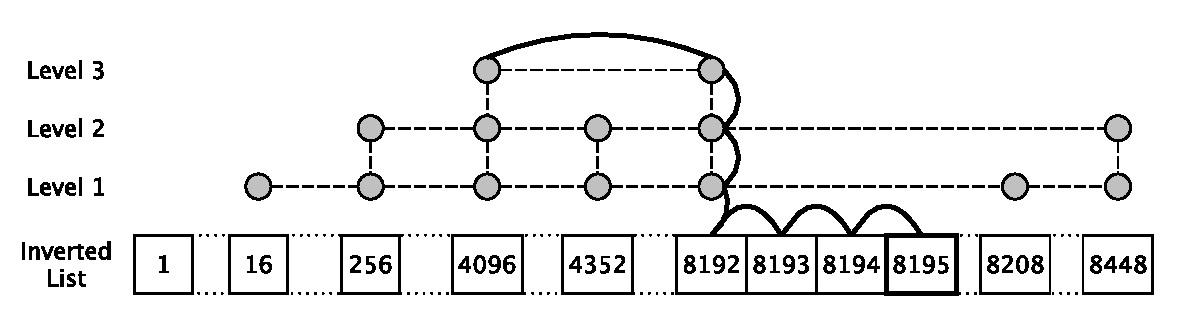
\includegraphics[scale=1]{pics/skiplists}
}%
\caption{Skip Lists with $p=\frac{1}{16}$. Dashed lines denote pointers between
synchronization points. The solid line shows the search path to the record 8195.}
\label{fig:skiplists}
\end{figure}

\section{Implementation}
 
 In this section we present the implementation of the Skip Lists structure as
 found in the open source project Apache Lucene\footnote{Apache Lucene:
 \url{http://lucene.apache.org/}}.
 
\paragraph{Structure}

The structure's data is kept on disk, and as such its implementation is done so
that the cost of IO operations are reduced. Each level of the Skip Lists is
stored as one stream, in order to read continuous data on disk when reading
synchronization points at a same level. The levels are stored one after the
other in reverse order, starting from the top level to level 1. The reverse
order storage of the levels is so that it maps the search algorithm flow, i.e.
we start on the top level, then descend levels to the bottom. The
Figure~\ref{fig:skiplists-impl} depicts the Skip Lists' Lucene implementation
of a synchronization point with 3 levels. The $ID$ refers to the record
identifier needed to advance in the Skip Lists. The \emph{Data} holds
information about the inverted list built upon such as file pointers. For a
same synchronization point such as in the figure, the Data block stores the same
information at each level about the inverted lists (i.e., duplicate data). The
next grey block depicts a file pointer, intern to the Skip Lists. This file
pointer stores the offset of a same synchronization point at the level below.
We can point out that for performance reasons, this file pointer points to the
end of a Data block, so that a duplicate information is not read twice when
descending levels.
 
\begin{figure}
\centering
\resizebox{0.6\linewidth}{!}{%
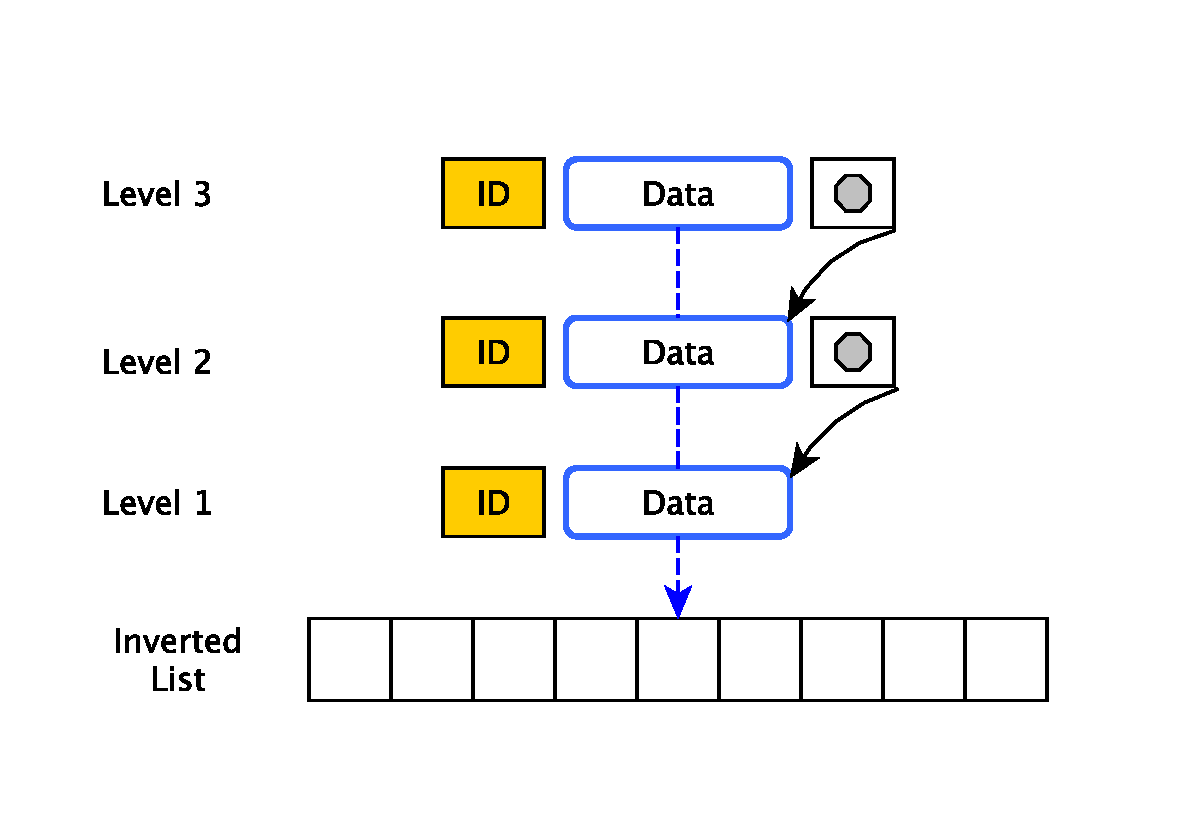
\includegraphics[scale=1]{pics/skiplists-impl}
}%
\caption{Skip Lists structure's implementation.}
\label{fig:skiplists-impl}
\end{figure}

\paragraph{Search algorithm}

The algorithm flow of the Skip Lists is highly optimized by having the less
branching conditions possible in order to maximizes the search throughput.
Given a targeted record that possibly is in the inverted list, the
\emph{\texttt{\#skipTo()}} method returns the interval that would hold it. On
the second line, the levels streams are loaded from disk if not done already.
The lines 4 to 6 walks up the levels as long as the current record identifier
of level i (i.e., stored within the \emph{currentIDs} variable) is lower than
the target. This allows to read only the levels that might skip to the target.
The loop starting at line 8 advances within the Skip Lists, by reading a
synchronization point at level i (line 10) as long as the current identifier is
lower than the target. On lines 12-13 we advance on the stream below to the
synchronization point which is the last being lower than the target.

\vspace{1em}
\begin{lstlisting}[frame=lines,language=Java,numbers=left,caption=Implementation of
the Skip Lists search
algorithm,label=lst:skiplists-search-algo,emph={currentIDs,moveToSynchronizationPoint,readSynchronizationPoint},
emphstyle={\bfseries}]
skipTo(int target)
	loadLevels();
	// Walk up the levels
	int level = 0;
	while (level < MAX_LEVELS - 1 && target > currentIDs[level + 1])
		level++;
	// Search for the interval containing the targeted record
	while (level >= 0) {
		if (target > currentIDs[level])
			readSynchronizationPoint(level)
		else
			moveToSynchronizationPoint(level-1);
			level--;
	}
\end{lstlisting}



\part{Methods}
\label{part:methods}
\chapter{Inverted Lists Compression For SIREn}{%
The SIREn indexing model generates a specific distribution of values. Since
each stream of values are local to an other (i.e attributes identifiers are
local to an entity, values identifiers are local to an attribute, and positions
are local to a value), a new compression algorithm that is better adapted to
the SIREn use case was researched.

The performance aspects looked after are
\begin{inparaenum}[(1)]
\item the compression
\item the decompression and
\item the compression ratio.
\end{inparaenum}
The decompression speed is important when processing queries because it means
that less time is to be spent on IO operations. The compression ratio is
important as per the storage space, but not only. As previously, less data
read from disk means less time wasted on IO operations. The compression speed
aspect does not matter when processing queries, but takes an important place
when updating the index. Indeed SIREn possesses an incremental index update
policy, thus compression algorithm showing good decompression speed will allow
indexes to be updated faster than an algorithm with slower compression
algorithm.

In this chapter, two of the compression techniques researched on are presented,
with \emph{RiceFOR} first, an algorithm that fuses together the Rice and FOR
algorithms, and the \emph{Adaptive Frame Of Reference} (AFOR), a new algorithm
based on FOR, which goal is to decrease the FOR sensibility to outliers.
}%
\label{chap:cmp-methods}
\section{RiceFOR}{
Rice is an algorithm that shows compression ratio
performance~\cite{zhang:2008:www} close to the interpolative coding, which is
an algorithm that provides the best compression ratio. However its complexity
is so high that it is used only as a comparison basis between algorithms.
RiceFOR is an attempt to take the best from both Rice and FOR algorithms: the
compression ratio of Rice and the highly CPU optimised FOR execution flow.
}

\subsection{Algorithm}

In the one hand, Rice computes the average of a block of values. Thanks to a
parameter $b$ being the power of 2 closest to this average, it computes the
Euclidean division of each values by b. The remainder is compressed using b
bits, and the quotient is encoded into an unary format. On the other hand, FOR
compress a block of values by applying a compression routine on sub-blocks of
32 integers, where the values across the sub-blocks are encoded into a same
number of bits. By computing the remainders in Rice all together, we achieve the
same use case as FOR, if the number of remainders is a multiple of 32.
The FOR algorithm is only used to compress with CPU optimized routines the
remainders. The compression ratio is the one that we can have thanks to Rice.

The RiceFOR algorithm works as follows. First we compute the remainders given a
parameter $b$ of all values to be compressed. We might have to add some fake
values (i.e., zeros) if the block's size is not a multiple of 32. These
remainders are outputted into a temporary block that will be compressed using
the FOR algorithm with b for the bit frame. Then the quotient of all values
are to be encoded with the unary format, as they would have been with the
original Rice algorithm.

The decompression algorithm works in the same way as the original Rice, the
difference being that the remainders are to be decompressed with FOR.

\subsection{Implementation}

Rice provides a good compression ratio~\cite{zhang:2008:www}, however the
computation of the statistics and unary encoding slow its compression and
decompression speed. Along with the optimization provided by the AFOR highly
performing routines, two optimized algorithms have been developed in order to
encode and decode efficiently values in unary format: an optimized routine to
encode a value into unary format, and a routine to decode unary values at the
byte level inspired from the Rice implementation in \cite{Yan:2009:sigir}.

\begin{description}
\item[Compression]
Using FOR to compress the remainders computed for the Rice
algorithm, RiceFOR is implemented as follows:
\begin{enumerate}
  \item[] Given a block B of integers
  \item the power of 2 directly lower to the mean of B is used as the bit frame.
  \item each sub-blocks of 32 remainders are compressed with that bit frame
  using the FOR routines such as the one presented in the
  Listings~\ref{lst:compression-routine}.
  \item the quotient of each integer (with the division by the bit frame) are
  encoded in unary format, using the optimized routine reported in the
  Listings~\ref{lst:optimized-unary-enc}.
\end{enumerate}
\item[Decompression] The remainders are decompressed with the
FOR routines, and the quotients are decoded using a byte-based decoding method
presented in the Listings~\ref{lst:block-unary-dec}. Indeed a byte is likely to
encode multiple values in unary format (e.g. 4 ones are encoded in one byte as
$0101\;0101$), thus it is possible to decode multiple values by reading a byte
a single time.
\end{description}

In the method \emph{encodeUnary} presented in the
Listings~\ref{lst:optimized-unary-enc}, the loop encode the quotient $q$ into
the array of byte $b$ of compressed data. The variable \emph{bit} is global and
records the number of bit already compressed. On line 3, the local variable
\emph{r} holds the number of bits in the current byte that are still unused.
The variable \emph{ones} holds the number of bits that will be set to 1. The
switch structure displays 8 hard coded cases to write from 1 to 8 bits at 1.
With the example of case 3 on line 7, the current byte, i.e., $bit / 8$, has
3 bits (7 in binary format: $111$) appended to it. These operations will repeat
until the quotient q has been completely encoded. The termination criterion of
the unary encoding, i.e., bit at zero, is computed on line 15. This suggests
that the current byte has been previously initialized to zero.

The method presented in the Listings~\ref{lst:block-unary-dec} reads a byte
containing values in unary format and decode them into an int array, starting
at the position \emph{offset}. All the unary encoded values are quotient
computed by the Rice algorithm, with a same parameter \emph{frameBit}. The
switch structure contains all 256 possibilities of bits configurations, and
hard codes for each cases the corresponding updates. For example the 26 case,
which in binary base equals $0001\;1010$, encodes 5 values which respectively
are from the least to the most significant bit $0$, $1$, $2$, 0 and 0. Thus the
quotients are respectively 0, $1^{bitFrame}$, $2\times1^{bitFrame}$, 0 and 0,
with $bitFrame$ the divisor parameter used in Rice.

\begin{fileformat}
  \centering
  \begin{minipage}[t]{0.47\linewidth}
\begin{lstlisting}[frame=lines,language=Java,numbers=left,caption=Unary
format encoding.,label=lst:optimized-unary-enc]
encodeUnary(int q, byte[] b)
	while (q > 0) {
		int r = 8 - (bit % 8);
		int ones = r > v ? v : r;
		switch (ones) {
			...
			case 3:
				b[bit / 8] |= (7 << (bit % 8));
				bit += 3;
				break;
			...
		}
		q -= ones;
	}
	bit += 1
\end{lstlisting}
  \end{minipage}
  \quad%
  \begin{minipage}[t]{0.47\linewidth}
\begin{lstlisting}[frame=lines,language=Java,numbers=left,caption=Byte-based
unary format decoding.,label=lst:block-unary-dec]
decodeUnary(byte b, int[] i)
	switch (b) {
		...
		case 26: // 26 = 0001 1010
			i[offset] += 0;
			i[offset + 1] += 1^frameBit;
			i[offset + 2] += 2*1^frameBit;
			i[offset + 3] += 0;
			i[offset + 4] += 0;
			offset += 5;
			break;
		...
	}
\end{lstlisting}
  \end{minipage}
\end{fileformat}

\section{Adaptive Frame Of Reference}{
The Adaptive Frame Of Reference (AFOR) attempts to retain the best of FOR,
i.e., a very efficient compression and decompression using highly-optimised
routines to avoid branching conditions, while providing a better tolerance
against outliers and therefore achieving a higher compression ratio. Compared
to PFOR, AFOR does not rely on the encoding of exceptions in the presence of
outliers. Instead, AFOR partitions a block into multiple frames of variable
length, the partition and the length of the frames being chosen appropriately
in order to adapt the encoding to the value distribution.
}
\label{sec:afor}

\subsection{Algorithm}

AFOR extends the FOR algorithm and runs as follows. Given a block $B$ of $n$
integers, AFOR partitions it into $m$ distinct frames and encodes each frame
using highly-optimised routines similarly to FOR. Each frame is independent
from one an other, i.e., each one has its own \emph{bit frame}, and each one
encodes a variable numbers of values. This is depicted in
Figure~\ref{fig:compression:afor} by \emph{AFOR-2}. AFOR encodes along with
the frame the associated bit frame with respect to a given encoder, e.g., a
binary encoder. In fact, AFOR encodes (respectively decodes) a block of values
by:
\begin{enumerate}
\item encoding (respectively decoding) the bit frame;
\item selecting the compression (respectively decompression) routine associated
to the bit frame;
\item encoding (respectively decoding) the frame using the selected routine.
\end{enumerate}

\begin{figure*}
  \centering
	\includegraphics[width=0.7\linewidth]{pics/afor-encoding}
	\caption{Block compression comparison between FOR and AFOR. We alternate
	colours to differentiate independent frames. AFOR-1 denotes a first
	implementation of AFOR using a fixed frame length. AFOR-2 denotes a second
	implementation of AFOR using variable frame lengths. AFOR-3 denotes a third
	implementation using variable frame lengths and the frame stripping technique.
 	\emph{BFS} denotes the byte storing the bit frame selector associated to the
	next frame.}
	\label{fig:compression:afor}
\end{figure*}

Finding the right partitioning, i.e., the optimal configuration of frames and
frame lengths per block, is essential for achieving high compression
ratio~\cite{rossano:2010:vse}. If a frame is too large, the encoding becomes
more sensitive to outliers and wastes bits by using a too big bit frame for
all the other integers. On the contrary, if the frames are too small, the
encoding wastes too much space due to the overhead of storing a larger numbers
of bit frames. The appropriate strategy is to rely 
\begin{enumerate}
  \item on large frames in the presence of a homogeneous sequence of values.
  \item on small frames in the presence of outliers.
\end{enumerate}
Also, alternating
between large and small frames is not only important for achieving high
compression ratio but also for achieving high performance. If the frames are
too small, the encoding has to perform more branching conditions to select the
appropriate routine for each bit frame, and therefore the compression and
decompression performance decrease. Therefore, it is better to rely on large
frames instead of multiple smaller frames when it is possible. Our solution
uses a greedy local optimization algorithm which is explained in the next
section.

\subsection{Partitioning Blocks into Variable Frames}

Finding the optimal configuration of frames and frame lengths for a block of
values is a combinatorial problem. For example, with three different frame
lengths (32, 16 and 8) and a block of size 1024 integers, there are $1.18
\times 10^{30}$ possible combinations. While such a combinatorial problem can
be solved via Dynamic Programming algorithms~\cite{rossano:2010:vse}, the
complexity of such algorithms is still $O(n \times k)$, with the term $n$
being the number of integers and the term $k$ the size of the largest frame,
therefore it greatly impacts the compression performance. Since we are not
only interested by a fast decompression speed and a high compression ratio,
but also by a fast compression speed, this approach is not used in our
experiments. Instead, we use a local optimization algorithm that provides a
satisfactory compression rate while being efficient to efficient to compute.

\begin{description}
\item[Local Optimization algorithm]
AFOR computes the block partitioning by using a sliding window over a block
and determines the optimal configuration of frames and frame lengths for the
current window.

Given a window of size $w$ and a list of possible frame
lengths, we first compute beforehand the possible configurations. For example,
for a window size of 32 and three different frame lengths, 32, 16 and 8, there
are six configurations: $[32],[16,16],[16,8,8],[8,16,8],[8,8,16],[8,8,8,8]$.
Then, given a list of possible configurations for a window, we
estimate the size of each configuration by doing one pass over the values of
the window as shown in the Algorithm~\ref{algo:afor2-opt} (Lines 1-5). This
first step performs $w \times k$ comparisons with $k$ the number of possible
configurations. The second step, Lines 6-12 in Algorithm~\ref{algo:afor2-opt},
performs a pass over the possible configuration and estimates the size of each
configuration in order to find the best one. The \texttt{EstimateSize}
function computes the cost of encoding the window given one configuration,
accounting also the overhead of storing the bit frames. For example, for the
configuration $[8,8,8,8]$ with four frames of size 8 each, and with four
associated bit frames, $b_{1}$ to $b_{4}$, the size of the encoding is
computed as follow: $4 + 8 \times \sum_{i=1\ldots4} log(b_i + 1)$, where $8
\times \sum_{i=1\ldots4} log(b_i + 1)$ is the size of the four encoded frames
and $4$ is the overhead to store the four bit frames.
\end{description}

This simple algorithm is efficient to compute, in particular if the
window size is small and the frame lengths are restricted to a few number.
However, it is easy to see that such method does not provide the optimal
configuration for a complete block. There is a trade-off between optimal
partitioning and complexity of the algorithm. However, one can possibly use a
more complex method for achieving higher compression ratio if the compression
speed is not critical. We decided to use this method since in our experiment
we found that a small window size of 32 values and three frame lengths, 32, 16
and 8, were providing satisfactory results in term of compression speed and
compression ratio. In the next Section is presented a more detailed explanation
of the AFOR implementation.

\SetAlFnt{\sf}
\IncMargin{.5em}
\begin{algorithm}
\SetAlgoLined
\LinesNumbered
\SetKwData{Conf}{c}
\SetKwData{BestConf}{bestConf}\SetKwData{BestSize}{bestSize}
\SetKwInOut{Input}{input}\SetKwInOut{Output}{output}
\SetKwFunction{GetBitFrame}{GetBitFrame}\SetKwFunction{SetBitFrame}{SetBitFrame}
\SetKwArray{BitFrames}{bitFrames}
\SetKwFunction{EstimateSize}{EstimateSize}

\Input{A window $W$ of size $w$}
\Input{The smallest frame length $l$}
\Output{The best configuration for the window}

\BlankLine
\BlankLine

\For{$i \leftarrow 0$ \KwTo $\frac{w}{l}$}{
  \For{$j \leftarrow i \times l$ \KwTo $(i + 1) \times l$}{
    \BitFrames{i} $\leftarrow \max($\BitFrames{i}$, \lceil \log_2(W[j] + 1) \rceil)$\;
  }
}
\BestSize $\leftarrow$ $MaxSize$\;
\ForEach{configuration \Conf of the possible configurations}{
  \If{\EstimateSize{\Conf, \BitFrames} $<$ \BestSize}{
    \BestSize $\leftarrow$ \EstimateSize{\Conf}\;
	\BestConf $\leftarrow$ \Conf\;
  }
}
\caption{The algorithm that finds the best configuration of frames and frame
lengths for a window $W$ of size $w$.}
\label{algo:afor2-opt}
\end{algorithm}
\DecMargin{.5em}

\subsection{Frame Stripping}
\label{sec:compression:stripping}

In an inverted list, it is common to encounter a long sequence of 1 to encode,
i.e., the delta gap value. For example, this occurs with terms that appear
frequently in many entities. With RDF data, such a very common term might be a
predicate URI or a widely present class URI. As a consequence, the list of
entity identifiers is composed of many consecutive identifiers, which is
encoded as a list of 1 using the delta representation. Also, the schema used
across the entity descriptions coming from a same dataset is generally
similar. When indexing batch of entities coming from a same dataset, we
benefit from a ``term clustering'' effect: all the schema terms are associated
with long runs of consecutive entity identifiers in the inverted index. There
is also other cases where a long run of 1 is common, for example in:
\begin{itemize}
\item the list of term frequencies for terms that appear frequently a single
time in the entity description, e.g., class URIs;
\item the list of value identifiers for terms that appear frequently in
single-valued attributes;
\item the list of term positions for nodes holding a single term, e.g., URIs. 
\end{itemize}

In presence of such long runs of 1, AFOR still needs to encode each value
using 1 bit. For example, a frame of 32 values will encode a sequence of 1
using 32 bits. The goal of the \emph{Frame Stripping} method is to avoid the
encoding of such frames. Our solution is to \emph{strip} the content of a
frame if and only if the frame is exclusively composed of 1. We encode such a
case using a special bit frame.

\subsection{Frame Skipping}
\label{sec:afor-skip}

Block-based compression techniques encode the configuration a block of integers
has been compressed with. When the length of the compressed block is unknown,
this compression header possesses information about the block that can be used
to skip this block and so not to decompress it.

With the AFOR algorithm, this method enables the possibility to skip a frame by
reading a BFS. This is not possible with techniques such as Rice, VByte or
PFOR. Since the BFS encodes the bit frame used to compress a frame, the size
in bytes of a compressed frame is found by the formula
\begin{displaymath}
\mid F \mid \times BFS
\end{displaymath}
where $\mid F \mid$ is the length of a frame. For instance the bit frame 1
(i.e., 1 bit) encodes a frame of 32 integers into 4 bytes.

With self-indexing structures (presented in Chapter~\ref{sec:self-indexing}),
the difference in bytes between two points in a stream is necessary in order to
know at which position data has to be read. These \emph{file pointers} have to
be stored, taking a considerable space. Thanks to the frame skipping method, it
is possible to get rid of the additional file pointers information, since the
size in bytes of a frame is known by reading its BFS.

\subsection{Implementations}

We present three different implementations of the AFOR encoder class. We can
obtain many variations of AFOR by using various sets of frame lengths and
different parameters for the partitioning algorithm. We tried many of them
during our experimentation and report here only the ones that are promising
and interesting to compare.

\paragraph{AFOR-1}

The first implementation of AFOR, referred to as AFOR-1 and depicted in
Figure~\ref{fig:compression:afor}, is using a single frame length of 32
values. To clarify, this approach is identical to FOR applied on small blocks
of 32 integers. This first implementation shows the benefits of using short
frames instead of long frames of 1024 values as in our original FOR
implementation. In addition, AFOR-1 is used to compare and judge the benefits
provided by AFOR-2, the second implementation using variable frame lengths.
Considering that, with a fixed frame length, a block is always partitioned in
the same manner, AFOR-1 does not rely on the partitioning algorithm presented
previously.

\paragraph{AFOR-2}

The second implementation, referred to as AFOR-2 and depicted in
Figure~\ref{fig:compression:afor}, relies on three frame lengths: 32, 16 and
8. We found that these three frame lengths give the best balance between
performance and compression ratio. Additional frame lengths were rarely
selected and the performance was decreasing due to the larger number of
partitioning configurations to compute. Reducing the number of possible frame
lengths was providing slightly better performance but slightly worse
compression ratio. There is a trade-off between performance and compression
effectiveness when choosing the right set of frame lengths. Our implementation
relies on the partitioning algorithm presented earlier, using a window's size
of 32 values and six partitioning configurations
$[32],[16,16],[16,8,8],[8,16,8],[8,8,16],[8,8,8,8]$.

\paragraph{AFOR-3}

The third implementation, referred to as AFOR-3 and depicted in
Figure~\ref{fig:compression:afor}, is identical to AFOR-2 but employs the
\emph{frame stripping} technique. Compared to AFOR-2, the compressed block can
contain frames which is then encoded by a single bit frame as depicted in
Figure~\ref{fig:compression:afor}. AFOR-3 implementation relies on the same
partitioning algorithm as AFOR-2 with an additional step to find and strip
frames composed of a sequence of 1 in the partitions.

\subsubsection{Compression and decompression routines}

Our implementations rely on highly-optimised routines such as the ones
presented in Listing~\ref{lst:compression-routine} and
\ref{lst:decompression-routine}, where each routine is loop-unrolled to encode
or decode a fixed number of values using shift and mask operations only. There
is one routine per bit frame and per frame length. For example, with a frame
length of 8 values, the routine encodes 8 values using 3 bits each as shown in
Listing~\ref{lst:compression-routine}, while for a frame length of 32, the
routine encodes 32 values using 3 bits each.

Since AFOR-1 uses a single frame length, it only needs 32 routines for
compression and 32 routines for decompression, i.e., one routine per bit frame
(1 to 32). With respect to AFOR-2, since it relies on three different frame
lengths, it needs 96 routines for compression and 96 routines for
decompression. As for AFOR-3, one additional routine for handling a
sequence of 1 is added per frame length. The associated compression routine is
empty and does nothing since the content of the frame is not encoded.
Therefore the cost is reduced to a single function call. The decompression
routine consists of returning an array of ones. This last routine is very fast
to execute since there are no shift or mask operations.

\subsubsection{Bit frame encoding}

As a reminder the bit frame is encoded along with the frame, so that, at
decompression time, the decoder can read the bit frame and select the
appropriate routine to decode the frame. In the case of AFOR-1, the bit frame
varies between 1 to 32. For AFOR-2, there are 96 cases to be encoded, where
cases 1 to 32 refer to the bit frames for a frame length of 8, cases 33 to 63
for a frame length of 16, and cases 64 to 96 for a frame length of 32. In
AFOR-3, we encode one additional case per frame length with respect to the
frame stripping method. Therefore, there is a total of 99 cases to be encoded.
The cases 97 to 99 refer to a sequence of 1 for a frame length of 8, 16 and 32
respectively.

In our implementation, the bit frame is encoded using one byte. While this
approach wastes some bits each time a bit frame is stored, more precisely 3
bits for AFOR-1 and 1 bit for AFOR-2 and AFOR-3, the choice is again for a
question of efficiency. Since bit frames and frames are interleaved in the
block, storing the bit frame using one full byte enables the frame to be
aligned with the start and the end of a byte boundary. Another implementation
to avoid wasting bits is to pack all the bit frames at the end of the block. We
tried this approach and report that it provides slightly better compression
ratio, but slightly worse performance. Since the interleaved approach was
providing better performance, we decided to use it in our benchmarks.

\subsubsection{Routine selection}

A precomputed lookup table is used by the encoder and decoder to quickly
select the appropriate routine given a bit frame. Compared to AFOR-1, AFOR-2
and AFOR-3 have to perform more table lookups for selecting routines since
they are likely to rely on small frames of 8 or 16 values when the value
distribution is sparse. While these lookups cost additional CPU cycles, we
will see in the experiments that the overhead is minimal.


\chapter{SkipBlock: Self-Indexing for Block-Based Inverted Lists}{%
SkipBlock is a model for block-based inverted lists, that can be applied as
well on traditional inverted lists. It is based on an adaptation of the Skip
List data structure. This work is orthogonal to related work on self-indexing
structures, since they might be extended to this model.

In this section, the SkipBlock model is presented with its associated search
algorithm. We discuss then the impact of the structure's parameters for both
Skip List and SkipBLock. We argue after the different strategies available to
search within intervals for both structures. Finally we compare thanks to a
cost-based model the differences between the Skip Lists and the SkipBlock. }
\label{chap:skipblock}
\section{The SkipBlock Model}
\label{sec:skipbock}

The Skip List model works on a record unit, i.e., a synchronization point has a
probability p to appear in an inverted list of n records.
The SkipBlock model operates instead on \emph{blocks} of records of a fixed
size, in place of the records themselves. Consequently, the probabilistic parameter
$p$ is defined with respect to a block unit. A synchronization point is
created every $\frac{1}{p^i}$ blocks on a level $i$, thus every $\frac{\vert B
\vert}{p^i}$ records where $\vert B \vert$ denotes the block size. A
synchronization point links to the first record of a block interval. Compared
to Figure~\ref{fig:skiplists}, a SkipBlock structure with $p=\frac{1}{8}$ and
$\vert B \vert=2$ also has an interval of $\frac{\vert B \vert}{p^1}=16$
records. However, on level 2, the synchronization points are separated by
$\frac{\vert B \vert}{p^2}=128$ instead of 256 records. We note that with
$\vert B \vert= 1$, the SkipBlock model is equivalent to the original Skip
Lists model, and therefore it is a generalization. The two properties of the
Skip Lists are then translated to this model:
\begin{enumerate}
  \item the number of levels is defined by
\begin{equation}
L_B(n)=\left\lfloor \ln_{\frac{1}{p}}\left(\frac{n}{\vert B \vert}\right) \right\rfloor
\label{eq:skipblock-maxlevels}
\end{equation}
  \item the structure's size
\begin{equation}
S_B(n)=\sum_{i=1}^{
L_B\left(n\right)}{\left\lfloor \frac{n\times p^i}{\vert B \vert}
\right\rfloor}
\label{eq:skipblock-size}
\end{equation}
\end{enumerate}

\subsection{SkipBlock Search Algorithm}
\label{sec:search-skipblock}

With the block-based Skip Lists model, the search algorithm returns an
interval of blocks containing the target record. We discuss the search in
that interval in Section~\ref{sec:search-interval}. The search walk is identical
to the one presented in Section~\ref{sec:search-skiplists}: we walk from the
top to the bottom level, and compare at each step the current synchronization
point with the target. The walk stops at the same termination criteria as in
Skip Lists. The search complexity in the worst case becomes
\begin{equation}
C_{SB}=\frac{L_B(n)}{p}
\label{eq:skipblock-complexity}
\end{equation}

\subsection{Impact of the Self-Indexing Parameters}
\label{sec:block-probas-impact}

In this section, we discuss the consequences of the probabilistic parameter on
the Skip Lists data structure.
Table~\ref{tab:skiplists-proba} reports for low (i.e., $\frac{1}{1024}$) and
high (i.e., $\frac{1}{2}$) probabilities
\begin{inparaenum}[(1)]
\item the complexity (\ref{eq:skiplists-complexity}) to find the interval
containing the target record, and
\item the size (\ref{eq:skiplists-size}) of the Skip Lists structure.
\end{inparaenum}
For example with an interval $\vert I \vert = 1024$ and an
inverted list of size $10^6$ (i.e., Skip Lists with one level), reaching a record
located at the end of the inverted list incurs a lot of synchronization points
at level 1 being read. With a smaller interval, e.g. 16, the number of
synchronization points read decreases because the $L(10^6)=4$ levels provide
more accessing points to the inverted list.

Large intervals give the possibility to skip over a large number of records by
reading a few synchronization points. However this leads to less use cases of
the Skip Lists structure when the searched records are close to each other. In
the latter case, small intervals are then more adapted, but at the cost of a
bigger structure. Moreover the more levels there are, the more walks up and
down on them there are.

There is a trade-off to achieve when selecting $p$: a high probability
provides a low search complexity but at a larger space cost, and a low
probability reduces considerably the required space at the cost of higher
search complexity.

The SkipBlock model provides two parameters to control its Skip Lists
structure: the probabilistic parameter $p$ and the block size $\vert B \vert$.
The block size parameter enables more control over the Skip Lists structure. For
example, to build a structure with an interval of length 64, the original Skip
Lists model proposes only one configuration given by $p=\frac{1}{64}$. For
this same interval length, SkipBlock proposes all the configurations that
verify the equation $\frac{\vert B \vert}{p}=64$.
Table~\ref{tab:skiplists-proba-block} reports statistics of some SkipBlock
configurations for the same interval lengths as in
Table~\ref{tab:skiplists-proba}. Compared to Skip Lists on a same interval
length, SkipBlock shows a lower search complexity in exchange of a larger
structure.

\begin{table}
\begin{center}
\subfloat[Skip Lists with $\vert I\vert=\frac{1}{p}$.]{
\centering
\ra{1.1}
\resizebox{0.39\linewidth}{!}{%
\begin{tabular}{@{}lcc@{\hs}c@{\hs}c@{\hs}c@{\hs}c@{\hs}}
\toprule
$\vert I \vert$ & \phantom{a} & 2 & 16 & 64 & 128 & 1024\\
\cmidrule{2-7}
$S(n)$ & \phantom{a} &
\numprint{99999988}&\numprint{6666664}&\numprint{1587300}&\numprint{787400}&\numprint{97751}\\
$C$ & \phantom{a} & 54 & 112 & 320 & 512 & 3072 \\
\bottomrule
\end{tabular}
\label{tab:skiplists-proba}
}}\quad%
\subfloat[SkipBlock with $\vert I\vert=\frac{\vert B \vert}{p}$.]{
\ra{1.1}
\resizebox{0.54\linewidth}{!}{%
\begin{tabular}{@{}lcc@{\hs}c@{\hs}cc@{\hs}c@{\hs}cc@{\hs}c@{\hs}cc@{\hs}c@{\hs}}
\toprule
$\vert I \vert$ & \phantom{a} & \multicolumn{2}{c}{16} & \phantom{a} &
\multicolumn{2}{c}{64} & \phantom{a} & \multicolumn{2}{c}{128} & \phantom{a} &
\multicolumn{2}{c}{1024} \\
\cmidrule{3-4} \cmidrule{6-7} \cmidrule{9-10} \cmidrule{12-13}
p:$\vert B \vert$ & \phantom{a} & $\frac{1}{4}$:4 & $\frac{1}{8}$:2 & \phantom{a} &
$\frac{1}{4}$:16 & $\frac{1}{8}$:8 & \phantom{a} & $\frac{1}{4}$:32 &
$\frac{1}{8}$:16 & \phantom{a} & $\frac{1}{4}$:256 & $\frac{1}{8}$:128 \\
$S_B(n)$ & \phantom{a} & \numprint{8333328} & \numprint{7142853} &
\phantom{a} & \numprint{2083328} & \numprint{1785710} & \phantom{a} &
\numprint{1041660} & \numprint{892853} & \phantom{a} &
\numprint{130203} & \numprint{111603} \\
$C$ & \phantom{a} & 48 & 64 & \phantom{a} & 44 & 56 & \phantom{a} &
40 & 56 & \phantom{a} & 36 & 48 \\
\bottomrule
\end{tabular}
\label{tab:skiplists-proba-block}
}}%
\end{center}
\caption{Search and size costs of Skip Lists and SkipBlock with $n=10^8$.
$\vert I \vert$ stands for an interval length. $C$ reports the search
complexity to find an interval (Sections~\ref{sec:search-skiplists}
and~\ref{sec:search-skipblock}).}
\end{table}

\section{Searching within an Interval}
\label{sec:search-interval}

The Skip Lists and SkipBlock techniques enables the retrieval of an interval
given a target record. The next step is to find the target record within that
interval. A first strategy (S1) is to linearly scan all the records within
that interval until the target is found. Its complexity is therefore $O(\vert I \vert)$.

SkipBlock takes advantage of the block-based structure of the
interval to perform more efficient search strategy. Here are defined four
additional strategies for searching a block-based interval, parameterized to a
probability p. The second strategy (S2) performs
\begin{enumerate}[(a)]
\item a linear scan over the blocks of the interval to find the block holding
the target and
\label{s2-linear-search-blocks}
\item a linear scan of the records of that block to find the target.
\label{s2-target-block}
\end{enumerate}
The search complexity is $\frac{1}{p}+\vert B \vert$ with $\frac{1}{p}$ denoting
the linear scan over the blocks and $\vert B \vert$ the linear scan over the
records of one block. Similarly to S2, the third strategy (S3) performs the
step (\ref{s2-linear-search-blocks}). Then, it uses to find the target an
inner-block Skip Lists structure restricted to one level only. The complexity
is $\frac{1}{p}+\frac{1}{q}+\left\lfloor\vert B\vert\times q\right\rfloor$
with q the probability of the inner Skip Lists. In contrast to S3, the fourth
strategy (S4) uses a non-restricted inner-block Skip Lists structure. The
complexity is $\frac{1}{p}+\frac{L(\vert B \vert)+1}{q}$ with q the inner Skip
Lists probability. The fifth one (S5) builds a Skip Lists structure on the
whole interval instead of on a block. Its complexity is then
$\frac{L\left(\frac{\vert B\vert}{p}\right)+1}{q}$, with $q$ the inner Skip
Lists probability. The strategies S3, S4 and S5 are equivalent to S2 when the
block size is too small for creating synchronization points.

\section{Cost-Based Comparison}
\label{sec:cost-based-cmp}

In this section, we define a cost model that we use to compare five
SkipBlock implementations and the original Skip Lists implementation.

\paragraph{Cost Model}
\label{sec:skipblock-cost-model}
For both the Skip Lists and the SkipBlock, we define a cost model by
\begin{inparaenum}[(a)]
\item the cost to search for the target, and
\label{cost-search}
\item the cost of the data structure's size.
\label{cost-size}
\end{inparaenum}
The search cost consists in the number of synchronization points traversed to
reach the interval containing the target, plus the number of records scanned
in that interval to find the target. The size cost consists in the total number
of synchronization points in the data structure, including the additional ones
for S3, S4 and S5 in the intervals.

\paragraph{Implementations}
\label{sec:impl} 
We define as the baseline implementation, denoted $I_1$, the Skip
Lists model using the strategy (\emph{S1}). We define
five implementations of the SkipBlock model, denoted by $I_2$, $I_3$,
$I_4$, $I_5$ and $I_6$, based on the five interval search strategies, i.e.,
\emph{S1}, \emph{S2}, \emph{S3},\emph{S4} and \emph{S5} respectively. The
inner Skip Lists in implementations $I_4$, $I_5$ and $I_6$ is
configured with probability $q=\frac{1}{16}$. The inner Skip Lists in $I_5$ and
$I_6$ have at least 2 levels. The size costs of the six implementations are 
\begin{itemize}
  \item[$I_1$:] $S(n)$
  \item[$I_2$:] $S_B(n)$
  \item[$I_3$:] $S_B(n)+\frac{n}{\vert B \vert}$
  \item[$I_4$:] $S_B(n)+\left\lfloor n\times q\right\rfloor$
  \item[$I_5$:] $S_B(n)+\frac{S(\vert B \vert)\times n}{\vert B \vert}$  
  \item[$I_6$:]$S_B(n)+\frac{S(p\times\vert B \vert)\times n}{p\times\vert B
  \vert}$
\end{itemize}

\paragraph{Comparison}

With respect to the SkipBlock model, we tested all the possible
configurations for a given interval length. We report that all of them were
providing better search cost than the baseline. We only report in
Table~\ref{tab:cmp-costs} the configurations providing the best search cost
given an interval length with the associated size cost. We observe that $I_2$
already provides better search cost than the baseline $I_1$ using the same
search strategy \emph{S1}, in exchange of a larger size cost. The other
implementations, i.e., $I_3$, $I_4$, $I_5$ and $I_6$ which use a more
efficient interval search strategies further decrease the search cost. In
addition, their size cost decreases significantly with the size of the
interval. On a large interval ($512$), $I_4$ is able to provide a low search
cost ($64$) while sustaining a small size cost ($6.5e6$). The inner Skip
Lists of $I_5$ and $I_6$ are built on lists too small to provide benefits. To
conclude, $I_4$ seems to provide a good compromise between search cost and
size cost with large intervals.

\begin{table}
\centering
\ra{1.1}
\resizebox{\linewidth}{!}{%
\begin{tabular}{@{}lcc@{\hs}c@{\hs}c@{\hs}c@{\hs}c@{\hs}c@{\hs}cc@{\hs}c@{\hs}c@{\hs}c@{\hs}c@{\hs}c@{\hs}cc@{\hs}c@{\hs}c@{\hs}c@{\hs}c@{\hs}c@{\hs}cc@{\hs}c@{\hs}c@{\hs}c@{\hs}c@{\hs}c@{\hs}}
\toprule
$\vert I\vert$&\phantom{a}&\multicolumn{6}{c}{8}
&\phantom{a}&\multicolumn{6}{c}{16}
&\phantom{a}&\multicolumn{6}{c}{512}
&\phantom{a}&\multicolumn{6}{c}{1152}\\
&\phantom{a}& $I_1$ & $I_2$ & $I_3$ & $I_4$ & $I_5$ & $I_6$  &\phantom{a}& $I_1$ & $I_2$ & $I_3$
& $I_4$ & $I_5$ & $I_6$   &\phantom{a}& $I_1$ & $I_2$ & $I_3$ & $I_4$ & $I_5$ & $I_6$  &\phantom{a}& $I_1$ &
$I_2$ & $I_3$ & $I_4$ & $I_5$ & $I_6$  \\
\cmidrule{3-8}\cmidrule{10-15}\cmidrule{17-22}\cmidrule{24-29}
SC&\phantom{a}& $72$ & $56$ & \multicolumn{4}{c}{$54$}
&\phantom{a}& $112$ & $62$ & \multicolumn{4}{c}{$56$}
&\phantom{a}& $1536$ & $548$ & $120$ & $64$ & $86$ & $84$
&\phantom{a}& $3456$ & $1186$ & $154$ & $74$ & $84$ & $81$ \\
\cmidrule{3-8}\cmidrule{10-15}\cmidrule{17-22}\cmidrule{24-29}
ZC$\times e6$&\phantom{a}& $14.3$ & $16.7$ & \multicolumn{4}{c}{$50.0$}
&\phantom{a}& $6.7$ & $12.5$ & \multicolumn{4}{c}{$25.0$}
&\phantom{a}& $0.2$ & $0.3$ &$1.8$ & $6.5$ & $7.0$ & $6.9$
&\phantom{a}& $0.09$ &$0.17$ & $1.7$&$6.4$ & $6.6$&$6.7$\\
\bottomrule
\end{tabular}
}%
\caption{Search (i.e., SC) and size (i.e., ZC, in million) costs with $n=10^8$.
SkipBlock implementations report the best search cost with the associated
size cost.}
\label{tab:cmp-costs}
\end{table}

\subsection{Skipping Analysis}

The SkipBlock structure, as a generalization of the Skip List, possesses the
same hierarchical layout. However the difference between the two is concrete:
SkipBlock jumps over groups of blocks at a time, whereas Skip Lists jumps over
groups of records. The Table~\ref{tab:skip-levels} reports the intervals at
each levels for both structures, with a constant interval between towers of
256 records. For a same interval length (e.g., 256 records in the table), we are
able to yield more configurations with the SkipBlock than with the Skip List
model. We remark that in both configurations of the SkipBlock, in-between
levels have been added in comparison to the original Skip List. These
additional levels give more skipping possibilities while searching. Moreover
this implies that more data will be read from a tower in a SkipBlock structure
than with the Skip List, for a same interval length.

\begin{table}
\ra{1.1}
\centering
\resizebox{0.45\linewidth}{!}{%
\begin{tabular}{lc@{\hs}rc@{\hs}rr}
\toprule
Level & \phantom{a} & Skip Lists & \phantom{a} & \multicolumn{2}{c}{SkipBlock}\\
\cmidrule{5-6}
& & p=256 & \phantom{a} & B=16 p=16 & B=64 p=4 \\
\cmidrule{5-6}
1 & \phantom{a} & 256 & \phantom{a} & 256 & 256 \\
2 & \phantom{a} & \uwave{\numprint{65536}} & \phantom{a} & \numprint{4096} &
\numprint{1024} \\
3 & \phantom{a} & \uwave{\numprint{16777216}} & \phantom{a} &
\uwave{\numprint{65536}} & \numprint{4096} \\
4 & \phantom{a} & \ldots & \phantom{a} & \numprint{1048576} & \numprint{16384}\\
5 & \phantom{a} & \ldots & \phantom{a} & \uwave{\numprint{16777216}} &
\uwave{\numprint{65536}}\\
\bottomrule
\end{tabular}
}
\caption{Interval length for each skip levels.}
\label{tab:skip-levels}
\end{table}

The SkipBlock structure will behave differently depending on the parameter
configurations in comparison to the Skip list, since they yield different skip
levels. To have a better understanding of the differences between the two
models, we discuss here the cost of reading skip data into memory and in which
case it outweighs the CPU saving thanks to an adaptation of the method from
\cite{moffat:96}.

Let $t_r$ be the cost of reading one record or a synchronization point, both as
part of a bulk read. Let also $t_d$ be the cost of decoding a
record/synchronization point. Let further $k$ be the number of
\emph{candidates}, i.e., the records that will be lookup from the inverted
list thanks to the self-indexing structure. Then the total time $T$ required
to search one inverted list of size $n$ in the worst case scenario (i.e., all
levels up to the maximum $L(n)$ are read) is given by the formula
\begin{displaymath}
T=T_d+T_r=kt_d\left( C + \vert I \vert \right)+t_r\left(n+2\times S\right) 
\end{displaymath}
where $T_d$ is the total time to decode pointers, $T_r$ the total time to read
into memory the inverted list and synchronization points. $ZC$ and $SC$ reports
respectively the size and the search costs. The numerical values of $t_d$ and
$t_r$ are respectively $2.5\times 10^{-6}$ and $0.5\times 10^{-6}$, values
taken from \cite{moffat:96}.

The Table~\ref{tab:predicted-times} reports a numerical comparison between the
two self-indexing models, with $n=60,000$ and $k=\{60,\;6000\}$. With a bigger
number of candidates we can expect a bigger processing time, since the
self-indexing structure will be accessed more often. The SkipBLock structure's
values are reported with the strategy S1 for the configurations that yields
the best processing time T. On small intervals (e.g., 16) the SkipBlock model
does not provide significant better performance even though the complexity is
better than the Skip List. This is explained by the difference in size, as the
amount of data to be read is greater, which is reflected by the greater
required time to read data $T_r$. As the interval increases, we can see that
the processing times increase for both models. However the expected
processing time is inferior with SkipBlock than with the original Skip List by
2 times.
The reason is that even if the strategies for searching within intervals is
the same (i.e., linear), the additional levels that the SkipBlock model
provides give more skipping possibilities. This comforts the fact that the
SkipBlock complexities are lower than the Skip List's. With the interval
$\vert I \vert = 1024$, the structure's size increases by 30\%, however both
the search complexity and the estimated processing time are twice as low as
the original model.

\begin{table}
\ra{1.1}
\centering
\resizebox{\linewidth}{!}{%
\begin{tabular}{lc@{\hs}rrrc@{\hs}rrrc@{\hs}rrc@{\whs}rrrc@{\hs}rrrc@{\hs}rr}
\toprule
$\vert I \vert$ & \phantom{a} & \multicolumn{10}{c}{Skip List} & \phantom{a} &
\multicolumn{10}{c}{SkipBlock} \\
\cmidrule{3-12} \cmidrule{14-23}
k &\phantom{a}& \multicolumn{3}{c}{60} &\phantom{a}& \multicolumn{3}{c}{6000}
&\phantom{a}& & & \phantom{a} & \multicolumn{3}{c}{60} &\phantom{a}&
\multicolumn{3}{c}{6000} & & \\
\cmidrule{3-5} \cmidrule{7-9} \cmidrule{14-16} \cmidrule{18-20}
& \phantom{a} & $T_d$ & $T_r$ & T & \phantom{a} & $T_d$ & $T_r$ & T &
\phantom{a} & SC & ZC & \phantom{a} & $T_d$ & $T_r$ & T & \phantom{a} &
$T_d$ & $T_r$ & T & \phantom{a} & SC & ZC \\
16&\phantom{a}&0.010&0.034&0.044
&\phantom{a}& 0.960 & 0.034 & 0.994 & \phantom{a}& 64 & 3998
&\phantom{a}&0.006&0.035&0.041
&\phantom{a}& 0.600 & 0.035 & 0.635 & \phantom{a}&40 & 4996 \\

32&\phantom{a}&0.019&0.032&0.051
&\phantom{a}& 1.92 & 0.032 & 1.952& \phantom{a} & 128 & 1934
&\phantom{a}&0.008&0.034&0.042
&\phantom{a}& 0.81 & 0.034 & 0.844 & \phantom{a}& 54 & 3743 \\

256&\phantom{a}&0.077&0.030&0.107
&\phantom{a}& 7.68 & 0.030 & 7.710& \phantom{a} & 512 & 234
&\phantom{a}&0.041&0.030&0.071
&\phantom{a}& 4.08 & 0.030 & 4.110& \phantom{a} & 272& 309 \\

512&\phantom{a}&0.154&0.030&0.184
&\phantom{a}& 15.36 & 0.030 & 15.390& \phantom{a} & 1024 & 117 
&\phantom{a}&0.079&0.030&0.109
&\phantom{a}& 7.89 & 0.030 & 7.920 & \phantom{a}& 526 & 229 \\

1024&\phantom{a}&0.307&0.030&0.337
&\phantom{a}&30.72 & 0.030 & 30.750& \phantom{a} & 2048 & 58
&\phantom{a}&0.155&0.030&0.185
&\phantom{a}& 15.54 & 0.030 & 15.570 & \phantom{a}& 1036 & 75 \\

\bottomrule
\end{tabular}}
\caption{Predicted processing times in seconds (n=60,000), with the
corresponding structure's search (i.e., SC) and size (i.e., ZC) costs. $T_d$
stands for the time for decoding a record, $T_r$ for the time of reading into memory a
record/synchronization point and T the sum of these two times. $k$ indicate the
number of candidates.}
\label{tab:predicted-times}
\end{table}


\part{Benchmarks}
\label{part:benchmarks}
\chapter{Benchmarking Framework}{
The benchmarks were all performed using JAVA, and some precautions should be
taken when doing so. Indeed JAVA is a language which is ``Just-In-Time'' (JIT)
compiled, meaning that the code used is compiled only at runtime. JAVA uses
different heuristics so that only the most frequently used code is compiled,
which optimizations take place while runtime. Thus the time spent by the Java
Virtual Machine (JVM) becomes a noise to benchmarks results evaluating the
running time of an application. This noise problem should be taken even more
seriously when performing micro-benchmarks in order to have sound results to
discuss on.

This Chapter presents the different points to pay attention to, before
describing the benchmarking platform used to get all the experiments results
in this report.
}
\label{chap:benchmarking-framework}
\section{JAVA and Benchmarking Pitfalls}

In this section, some of the important points to take care of in
micro-benchmarking with JAVA are presented. The implementation of our benchmark
platform is based on the technical advices from \cite{boyer:2008:bench}, where
more details about the technical aspects can be found.

\begin{description}
\item[Time recording] With micro-benchmarking, the running time is generally
below 10 ms. Thus using the method \#System.currentTimeMillis() is not adapted.
An other method for recording such short running times is available within that
same class, \#System.nanoTime(), which gives a time at the nano-second precision.
\item[Warm up] The JVM works on the code while it is being run. Indeed the JVM
is based on just-in-time (JIT) compilation, thus the JVM performs some
optimizations on the code at runtime, thanks to various statistics gathered. In
order to decrease the noise because of those heuristics, the portion of code
being evaluated has to be run several times, without any measures being
recorded. In doing so, the classes that are used during the benchmark are
already ``loaded'' by the JVM. \cite{boyer:2008:bench} reports that doing so for
10 seconds is enough to have most of the JVM optimizations done.
\item[Dynamic optimization] Even though the warm up phase decreases the number
of optimizations likely to be done by the JVM hereafter, it is still possible
that some are executed while measuring the running time. In order to detect
these changing state of the JVM, we can use the JAVA classes
\emph{ClassLoadingMXBean} and \emph{CompilationMXBean} within the package
``java.lang.management'' that reports various statistics about the JVM, e.g. the
number of loaded classes.

On line 2 and 3, we instantiate objects that gives information about the state
of the JVM. ClassLoadingMXBean reports the number of classes that have been
loaded/unloaded since the JVM started. CompilationMXBean reports the time
ins ms spent on compilation. By wrapping the evaluated code with such
recordings of the JVM (lines 5 to 7 and 13 to 15), we are able to detect that
the JVM performed an optimization by testing those variables: if they are
different, the JVM state changed and so the evaluation need to be restarted.
This allows to make sure that the evaluated time returned is as ``clean'' as
possible.
\lstset{basicstyle=\small,language=Java,commentstyle=\color{red},
emph={ClassLoadingMXBean,CompilationMXBean},emphstyle=\color{blue}}
\begin{lstlisting}[frame=single,numbers=left]
// MF is the namespace used for ManagementFactory
ClassLoadingMXBean loadBean = MF.getClassLoadingMXBean();
CompilationMXBean compBean = MF.getCompilationMXBean();

long loadedClasses1 = loadBean.getTotalLoadedClassCount();
long unloadedClasses1 = loadBean.getUnloadedClassCount();
long compiledTime1 = compBean.getTotalCompilationTime();

long t1 = System.nanoTime();
// Evaluated Code
long t2 = System.nanoTime();

long loadedClasses2 = loadBean.getTotalLoadedClassCount();
long unloadedClasses1 = loadBean.getUnloadedClassCount();
long compiledTime2 = compBean.getTotalCompilationTime();
\end{lstlisting}
\item[Memory management] The memory usage of an application is managed by the
JVM through the use of two mechanisms that are automatically executed. The user
as no control over them and can occur any time the JVM deems necessary.
\begin{enumerate}
  \item {\bfseries Garbage Collection:} free the allocated memory by objects
  that are no more used. It can be explicitly called by \emph{\#System.gc()}.
  \item {\bfseries Object Finalization:} any objects possess the
  \#finalize() method, which frees all resources used by this object. This
  method is called by the garbage collection mechanism. However it is possible
  to explicitly run this method for all objects which destruction is pending by
  calling the method \emph{\#System.runFinalization()}.
\end{enumerate}
The time spent on running those two mechanisms is an other source of noise in
the benchmark. This can be prevented to some point by calling the \#System.gc()
and \#System.runFinalization() methods until the memory usage stabilizes.

The loop from line 11 to 24 tries to free by force with calls to the previous
presented methods. The loop is repeated until the consumed memory stabilizes
and that the number of objects that are waiting to be destroyed are no more.

\lstset{basicstyle=\small,language=Java,commentstyle=\color{red},
emph={gc,runFinalization},emphstyle=\color{blue}}
\begin{lstlisting}[frame=single,numbers=left]
// Return the amount of memory currently used
long usedMem() {
  final Runtime rt = Runtime.getRuntime();
  return rt.totalMemory() - rt.freeMemory();
}
   
final MemoryMXBean mem = ManagementFactory.getMemoryMXBean();
long usedMemPrev = usedMem();

// Upper bound of 100 iterations in order to prevent an ininite loop
for (int i = 0; i < 100; i++) {
  // Trying to free memory 
  System.runFinalization();
  System.gc();

  final long usedMem Now = usedMem();
  // Return the number of objects waiting for finalization
  final int county = mem.getObjectPendingFinalizationCount();

  if ((oCount == 0) && (usedMemNow >= usedMemPrev)) // Memory usage stable
    break;
  else
    usedMemPrev = usedMemNow;
}
\end{lstlisting}
\end{description}

\section{Experimental Environment}

In this section is presented the benchmarking framework that is used for all
benchmarks results presented in the next chapters.

\paragraph{Experimental Settings}

The hardware system we use in our experiments is a 2 x Opteron 250 @ 2.4 GHz
(2 cores, 1024 KB of cache size each) with 4GB memory and a local 7200 RPM
SATA disk. The operating system is a 64-bit Linux 2.6.31-20-server. The
version of the Java Virtual Machine (JVM) used during our benchmarks is
1.6.0\_20. The compression algorithms and the benchmark platform are written
in Java and based on the open-source project Apache Lucene\footnote{Apache
Lucene: \url{http://lucene.apache.org/}}.

\paragraph{Experimental Design}

The benchmarking design below takes into consideration the different critical
points that were previously presented. Each evaluation of the benchmark where
made by
\begin{quote}
\begin{enumerate}
  \item[Initialisation of the benchmark environment]
  \item flushing the OS cache;
  \item initialising a new JVM; 
  \item warming the JVM by executing a certain number of times the benchmark
  until 10 seconds is reached.

  \item[Evaluation of the benchmarked code]
  \item Each measurement is made by performing $n$ times the evaluated code
  execution, with $n$ chosen so that the runtime is long enough to minimise the
  time precision error of the OS and machine (which can be 1 to 10
  milliseconds) to a maximum of 1\%. The measurement time is the CPU time,
  i.e., user time and system time, used by the current thread.
  \item the previous step is re-run if the JVM state changed.
  \item the average running time is recorded.

  \item steps from 4 to 6 are repeated 100 times.
  \item[] As recommended in \cite{lilja:2000:book}, we report the harmonic mean
  and the standard deviation of the 100 measurements.
\end{enumerate}
\end{quote}
The JVM warmup is necessary in order to be sure that the OS and the JVM have
reached a steady state of performance, e.g., that the critical portion of code
is JIT compiled by the JVM.

\subsection{Measurements}

The benchmark produces 100 measurements for one evaluation so that an average
running time can be given, with its standard deviation. However one has to be
wary regarding such results. Indeed while the standard deviation allows to have
a better critic about the running time, it can also lead to misinterpretations.

The \emph{Vysochansk\"i-Petunin} inequality shows that 95\% of the measurements
lie within an interval of three times the standard deviation around the mean.
When comparing two different evaluations with these statistics, one cannot say
which one is faster if that interval around the mean overlaps. The
Figure~\ref{fig:non-overlapping-means} depicts the case where two evaluations
have their intervals non-overlapping, in which case it is possible to say that
the evaluation with the lower mean is better. However this is not the case if
intervals do overlap, as it is the case in the
Figure~\ref{fig:overlapping-means}. Indeed we can have a measurement belonging
to evaluation 2 faster than one from the evaluation 1, even though the mean of
evaluation 1 is lower than the mean of evaluation 2. In such a case, we cannot
say which one is faster, only that the two evaluated codes are similar.

\begin{figure}
\resizebox{\linewidth}{!}{%
\subfloat[Non-overlapping standard deviations.]{%
\centering
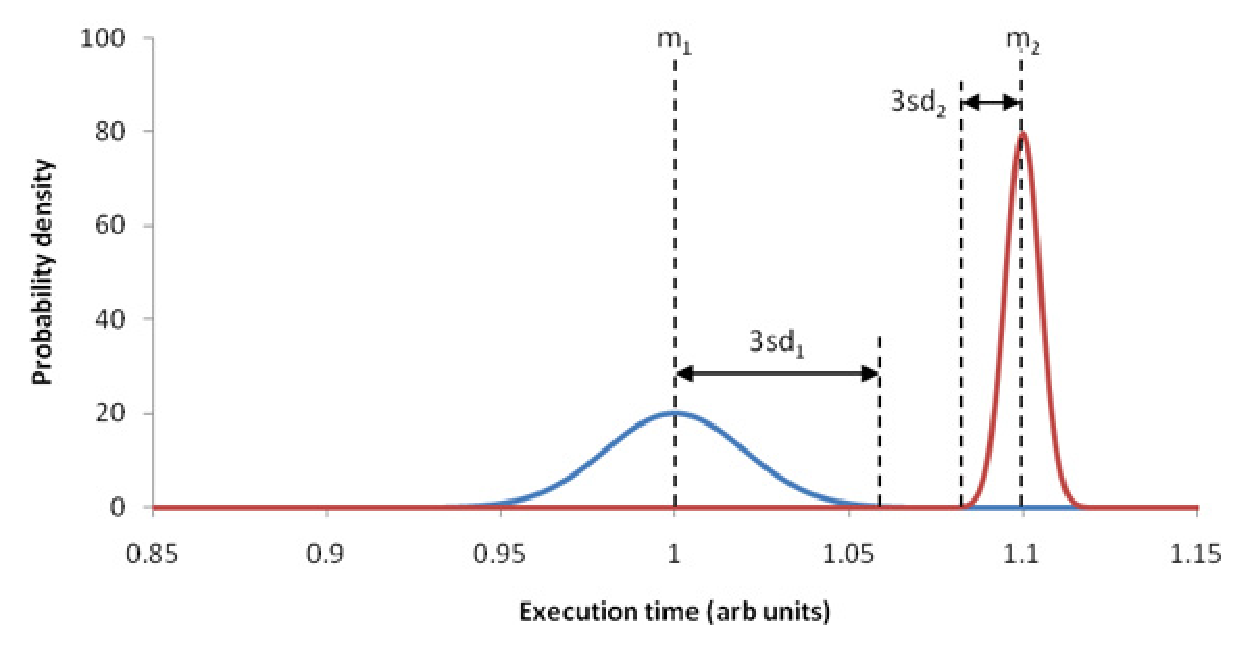
\includegraphics[scale=0.47]{pics/non-overlaping-means}
\label{fig:non-overlapping-means}
}\quad
\subfloat[Overlapping standard deviations.]{%
\centering
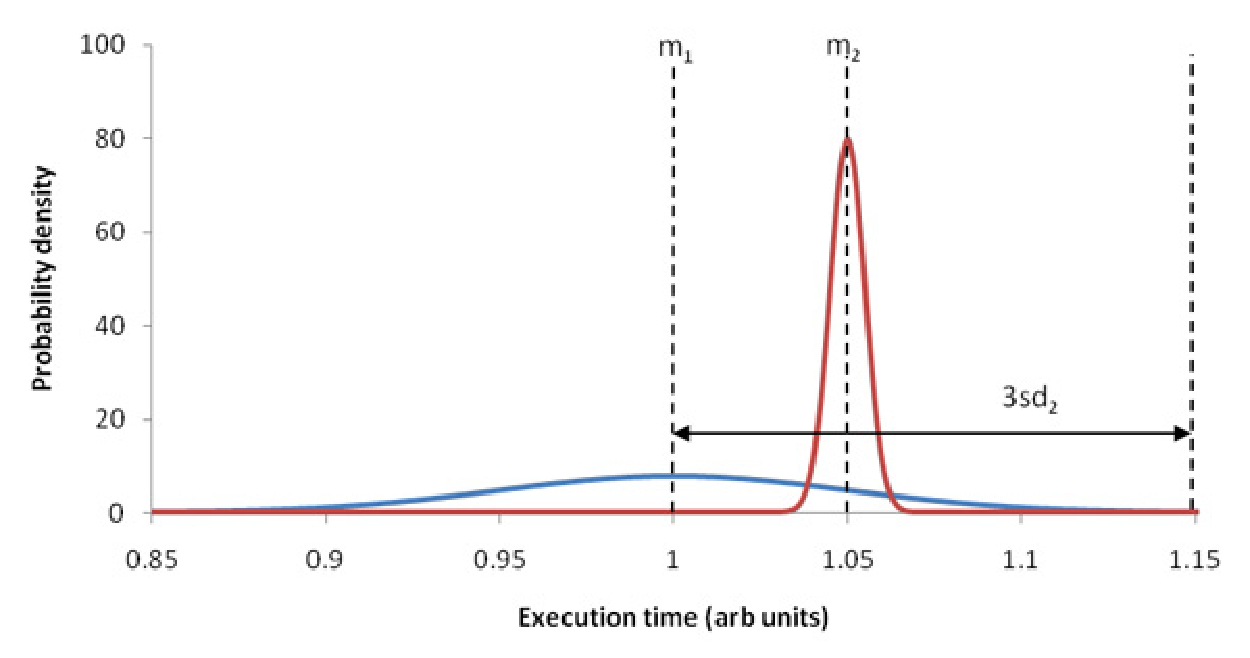
\includegraphics[scale=0.47]{pics/overlaping-means}
\label{fig:overlapping-means}
}}%
\caption{Benchmarks results of two measurements reported with means ($m_i$) and
standard deviations ($sd_i$).}
\end{figure}

% Since the conclusions that we can drawn from the results are based on the mean
% and the standard deviations values, we need to know how much reliability we can
% put into them. Because of all the points that have to be taken care of while
% benchmarking, it is not impossible that some noise still persists while the
% evaluation. With the set of 100 measurements, there are two techniques that can
% inform on the reliability aspect of the statistics, \emph{confidence
% intervals}~\cite{boyer:2008:bench} and the \emph{ANOVA}~\cite{lilja:2000:book} method.
% \begin{description}
% \item[confidence intervals] Means and standard deviations are single computed
% value (i.e. a point estimate), and another run of the benchmark might output
% other results for some reason (e.g. maintenance operations by the system,
% outside of a user control). On the opposite, confidence intervals give a range
% of estimates. A probability p called the confidence level is associated with
% this range. Most commonly, p is chosen to be 95\% and is kept constant during
% confidence interval comparisons. Confidence intervals are intuitive because
% their size indicates reliability: short intervals indicate that the statistic
% is precisely known, while wide intervals indicate uncertainty. For example, if
% the confidence interval for the mean execution of task A is [1, 1.1]
% milliseconds, and that for task B is [0.998, 0.999] milliseconds, then B's
% mean is known with more certainty than A's and is also distinguishably smaller
% (at the same confidence level).
% Confidence intervals can be computed thanks to the
% \emph{bootstrapping}\footnote{Boostrapping:
% \url{http://en.wikipedia.org/wiki/Bootstrapping_(statistics)}} technique, that
% can work for any statistics. A precise explanation of this technique is outside
% the scope of this report.
% \item[ANOVA] Given a set of algorithms to be evaluated, we run them on our
% benchmark and compute for each algorithm a set of 100 measurements. As depicted
% in the Figure~\ref{fig:overlapping-means}, we cannot state with certainty that
% an algorithm A is better than an algorithm B if their interval given by the
% \emph{Vysochansk\"i-Petunin} inequality overlaps. Moreover the difference
% between two algorithms in the other case might not be real if there was some
% noise. \emph{Analysis of the Variance} is a statistical method that tells at
% some confidence degree if one evaluation is statistically better than an other
% one. Thus we can state clearly that an algorithm A is statiscally faster than an
% algorithm B, meaning that the difference observed between the two are real and
% not the consequence of some noise while benchmarking. 
% \end{description}
% ANOVA makes the assumption that measures noises are independent from one
% evaluation to another and that they follow a Gaussian law, while confidence
% intervals does not make any assumptions about the underlaying data.


\chapter{Compression Benchmarks}{
This section describes the benchmark experiments which aim to compare the
various compression methods described previously. The benefits gained with the
use of AFOR algorithms is discussed through two types of data sources. The
first one are unstructured documents: a document is just a bag of words. The
second one are semantically structured documents, e.g. RDF enriched documents.
Since the indexing model for these two types are different, the distribution of
the values within the streams is then also different. Thus the efficiency of a
same compression technique depends on the dataset type.
}
\label{chap:benchmark-cmp}
\section{Benchmarks Settings}
\label{sec:benchmark:framework-cmp}

This section describes the benchmark experiments which aim to compare the
techniques introduced by AFOR with the compression methods described in
Section~\ref{sec:compression:state-of-the-art}. The first experiment measures
the indexing performance based on two aspects:
\begin{inparaenum}[(1)]
\item the indexing time; and 
\item the index size. 
\end{inparaenum}
The indexing time corresponds to the time required to build the index, be it a
traditional inverted index or a node-based inverted index like SIREn. As for
the index size, this time will vary with the compression technique used. The
second experiment compares the query execution performance using indexes built
with different compression techniques.

\paragraph{Data Collection}

In these benchmarks, five datasets were used. Two of them are plain text
datasets which will be used to build traditional inverted indexes, while the
three others are RDF triples and so will be used to build SIREn indexes.

\begin{quotation}
$\Longrightarrow$ Datasets for traditional indexes are composed of:
\begin{description}
\item[Wikipedia:] set of English language Wikipedia articles (~2.5 million
articles). Its total size is 42GB uncompressed.
\item[Blog:] set of 44 million blog posts made between August 1st and October
1st, 2008~\cite{burton:2009:spinn3r}. Its total size is 142GB uncompressed.
\end{description}
\end{quotation}

\begin{quotation}
$\Longrightarrow$ Datasets for the SIREn structure are the following three:
\begin{description}
\item[Geonames:] a geographical database and contains 13.8 million of
entities\footnote{Geonames: \url{http://www.geonames.org/}}. The size is 1.8GB
compressed.
\item[DBPedia:] a semi-structured version of Wikipedia and contains 17.7
million of entities\footnote{DBpedia: \url{http://dbpedia.org/}}. The size is
1.5GB compressed.
\item[Sindice:] a sample of the data collection currently indexed by Sindice.
There is a total of 130.540.675 entities. The size is 6.9GB compressed.
\end{description}
We extracted the entity descriptions from each dataset as pictured in
Figure~\ref{fig:entities}.
\end{quotation}

\section{Indexing Performance}
\label{sec:compression:indexing-performance}

The performance of indexing is compared based on the index size (compression
ratio), commit time (compression speed) and optimise time (compression and
decompression speed). The indexing is performed by adding incrementally 10000
documents at a time and finally by optimising the index.

We report the results of the indexing experiments in
Table~\ref{tab:indexing-performance}. The table comprises two columns with
respect to the indexing time: the total commit time (\emph{Total}) to add all
the documents and the optimisation time (\emph{Opt}). The time collected is
the CPU time used by the current thread and comprises the user time and the
system time. The index size in Table \ref{tab:indexing-performance} is studied
based on the size of each values' streams in the inverted file, and on the total
size of the index. For indexes built with unstructured data (i.e. Wikipedia and
Blog), these streams represent the document identifier, the frequency and the
positions. As for the indexes built on structured data (i.e. DBpedia, Geonames,
Sindice), the streams represent the entity, frequency, attribute, value and
position values. In each tables, the total size is computed by summing the size
of each streams. Bar plots are also provided in order to visualise better the
differences between the techniques.

\paragraph{Commit Time}

Figure~\ref{fig:commit-time} shows the total time spent by each method. As
might be expected, Rice is the slowest method due to its execution flow
complexity on both source type.

On the large unstructured dataset Blog, PFOR is equivalent to Rice in term of
compression speed, since PFOR spends more time in finding the outliers. AFOR-2
and S-64 perform similarly, while AFOR-1 performs as fast as VByte. The drop of
efficiency between AFOR-2 and AFOR-1 is due to the optimization algorithm to
find the best compressing frame. On the small dataset Wikipedia, Rice is
followed by S-64. While FOR, PFOR and VByte perform similarly, AFOR-1 and
AFOR-2 algorithms are the most efficient methods.

On small structured datasets (DBpedia and Geonames), algorithms behave
similarly as described previously. AFOR-3 shows equivalent performance as S-64
on DBpedia, while performing as the best one on Geonames. On a large dataset
(Sindice), VByte is the best-performing method while AFOR-1, AFOR-2, AFOR-3
and S-64 provide a similar commit time. On large datasets (Sindice and Blog),
VByte provides the best commit times, reflecting the benefit from a simple
algorithm.

\begin{figure}
  \centering
    \resizebox{0.8\linewidth}{!}{%
    % \subfloat[Unstructured data]{%
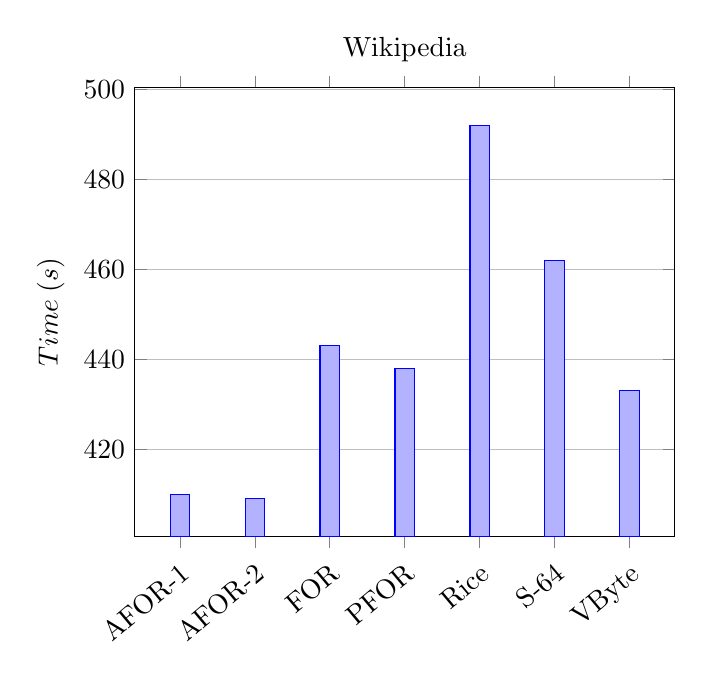
\begin{tikzpicture}[baseline]
\begin{axis}[
ylabel=$Time \; (s)$,
x tick label style={rotate=40, anchor=north east},
xtick={1,...,7},
xticklabels={AFOR-1, AFOR-2, FOR, PFOR, Rice, S-64, VByte},
legend style={at={(0.5,1.13)}, anchor=north, legend columns=-1},
ybar,
ymajorgrids=true,
bar width=7pt,
%enlargelimits=0.015,
title={Wikipedia}
]

\addplot
coordinates {(1, 410) (2, 409) (3, 443) (4, 438) (5, 492) (6, 462) (7, 433)};

\end{axis}
\end{tikzpicture}

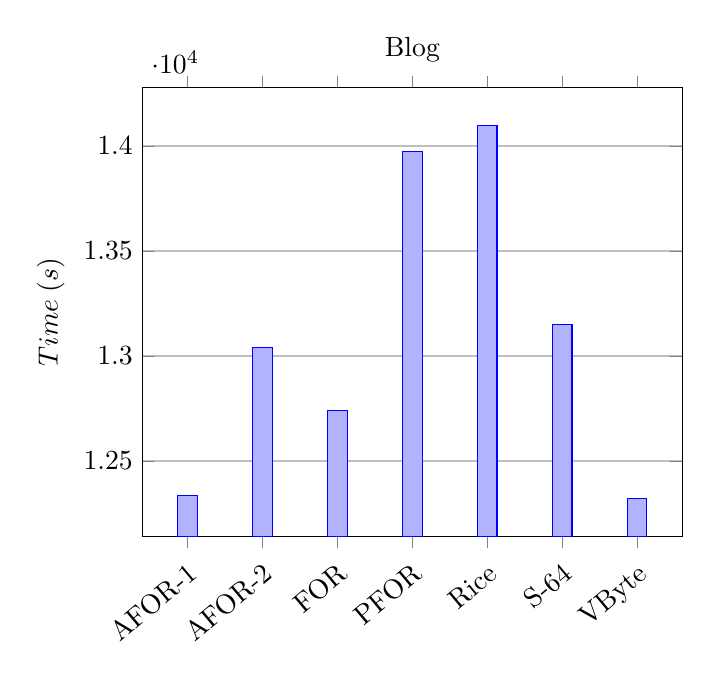
\begin{tikzpicture}[baseline]
\begin{axis}[
ylabel=$Time \; (s)$,
x tick label style={rotate=40, anchor=north east},
xtick={1,...,7},
xticklabels={AFOR-1, AFOR-2, FOR, PFOR, Rice, S-64, VByte},
legend style={at={(0.5,1.13)}, anchor=north, legend columns=-1},
ybar,
ymajorgrids=true,
bar width=7pt,
%enlargelimits=0.015,
title={Blog}
]

\addplot
coordinates {(1, 12337) (2, 13040) (3, 12741) (4, 13972) (5, 14099) (6, 13152) (7, 12320)};

\end{axis}
\end{tikzpicture}
% }
  }
\quad
  \resizebox{\linewidth}{!}{%
    % \subfloat[Structured data]{%
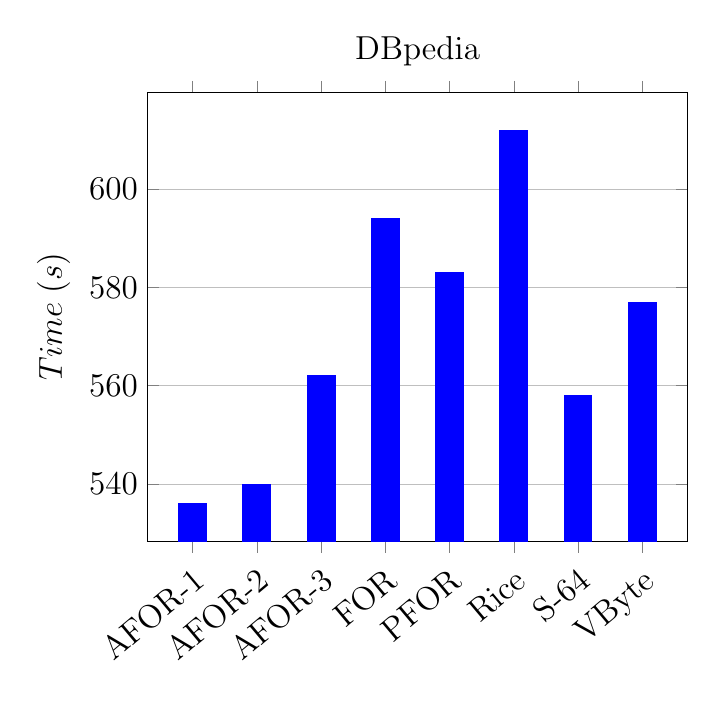
\begin{tikzpicture}[baseline]
\begin{axis}[
ylabel=$Time \; (s)$,
x tick label style={font=\large, rotate=40, anchor=north east},
xtick={1,...,8},
xticklabels={AFOR-1, AFOR-2, AFOR-3, FOR, PFOR, Rice, S-64, VByte},
legend style={at={(0.5,1.13)}, anchor=north, legend columns=-1},
label style={font=\large},
tick label style={font=\large},
title style={font=\large},
ybar,
ymajorgrids=true,
bar width=10pt,
title={DBpedia},
%enlargelimits=0.15,
]
\addplot[draw=blue,fill=blue]
coordinates {(1, 536) (2, 540) (3, 562) (4, 594) (5, 583) (6, 612) (7, 558) (8, 577)};
%\legend{Wikipedia}
\end{axis}
\end{tikzpicture}%
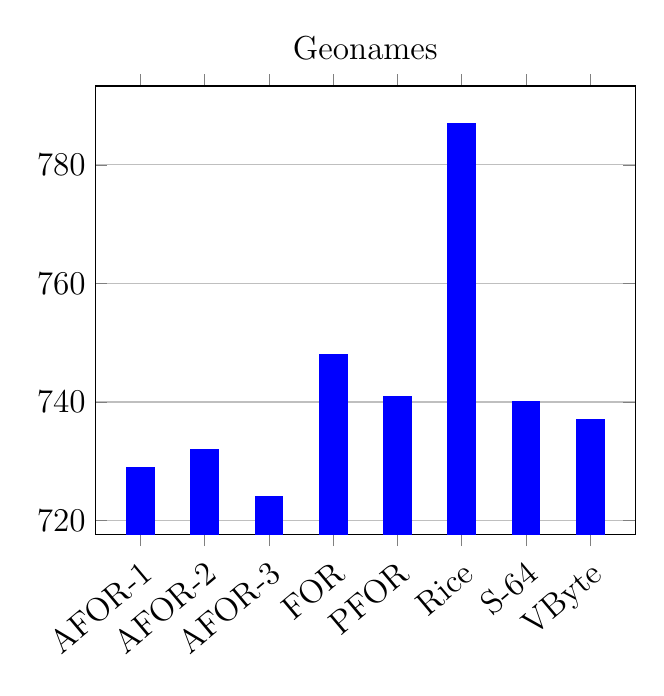
\begin{tikzpicture}[baseline]
\begin{axis}[
x tick label style={font=\large, rotate=40, anchor=north east},
xtick={1,...,8},
xticklabels={AFOR-1, AFOR-2, AFOR-3, FOR, PFOR, Rice, S-64, VByte},
legend style={at={(0.5,1.13)}, anchor=north, legend columns=-1},
label style={font=\large},
tick label style={font=\large},
title style={font=\large},
ybar,
ymajorgrids=true,
bar width=10pt,
title={Geonames},
%enlargelimits=0.15,
]
\addplot[draw=blue,fill=blue]
coordinates {(1, 729) (2, 732) (3, 724) (4, 748) (5, 741) (6, 787) (7, 740) (8, 737)};
%\legend{Blog}
\end{axis}
\end{tikzpicture}
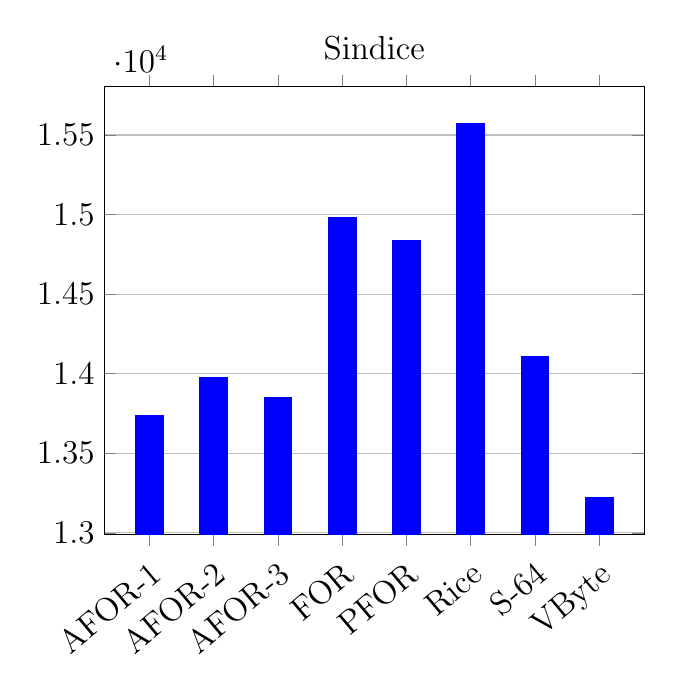
\begin{tikzpicture}[baseline]
\begin{axis}[
x tick label style={font=\large, rotate=40, anchor=north east},
xtick={1,...,8},
xticklabels={AFOR-1, AFOR-2, AFOR-3, FOR, PFOR, Rice, S-64, VByte},
legend style={at={(0.5,1.13)}, anchor=north, legend columns=-1},
label style={font=\large},
tick label style={font=\large},
title style={font=\large},
ybar,
ymajorgrids=true,
bar width=10pt,
title={Sindice},
%enlargelimits=0.15,
]
\addplot[draw=blue,fill=blue]
coordinates {(1, 13734) (2, 13975) (3, 13847) (4, 14978) (5, 14839) (6, 15571) (7, 14107) (8, 13223)};
%\legend{Blog}
\end{axis}
\end{tikzpicture}
% }
  }
	\caption{The total time spent to commit all the batches of 10000 document.}
	\label{fig:commit-time}
\end{figure}

\paragraph{Optimisation Time}

Figure~\ref{fig:optimise-time} shows the optimise time for each methods. The
time to perform the optimisation step is quite different due to the nature of
the operation. The optimisation operation has to read and decompress all the
index segments and compress them back into a single segment. Therefore,
decompression performance is also an important factor, and algorithms having
good decompression speed becomes more competitive.

On both data sources types, while PFOR was similar to Rice in term of commit
time on large datasets (Blog and Sindice), it is ahead of Rice in term of
optimisation time. This can be seen too with FOR on Sindice only. Rice is
penalised by its low decompression speed. The difference introduces by the
decompression performance can also be seen with S-6, which provides performance
close to or even better than VByte. While VByte performs fairly well on
unstructured data, we notice a large overhead on Sindice. The reason is the
distribution of the values on each stream: SIREn produce small values, since
there is a locality effect, i.e. attributes are local to an entity, values are
local to an attribute and positions are local to a value. On traditional
inverted index, position values are local to the whole document, and are then
much bigger. The Table~\ref{tab:indexing-performance} reports a positions
stream of size 20 GBytes at least with every compression techniques, while the
SIREn's streams sizes are bellow 2 GBytes. This difference in compression
ratio produce a large overhead on large datasets (Sindice) with the
decompression speed of VByte.

The best-performing methods are AFOR-1, AFOR-2 and AFOR-3 (structured data
only), with AFOR-3 performing better on large datasets. The AFOR techniques
take the advantage due their optimised compression and decompression routines
and their good compression rate. AFOR-3 is even twice as fast as Rice on the
Sindice dataset.

\begin{figure}
\centering
\begin{minipage}{0.8\linewidth}
  \centering
    \resizebox{0.7\linewidth}{!}{%
    % \subfloat[Unstructured data]{%
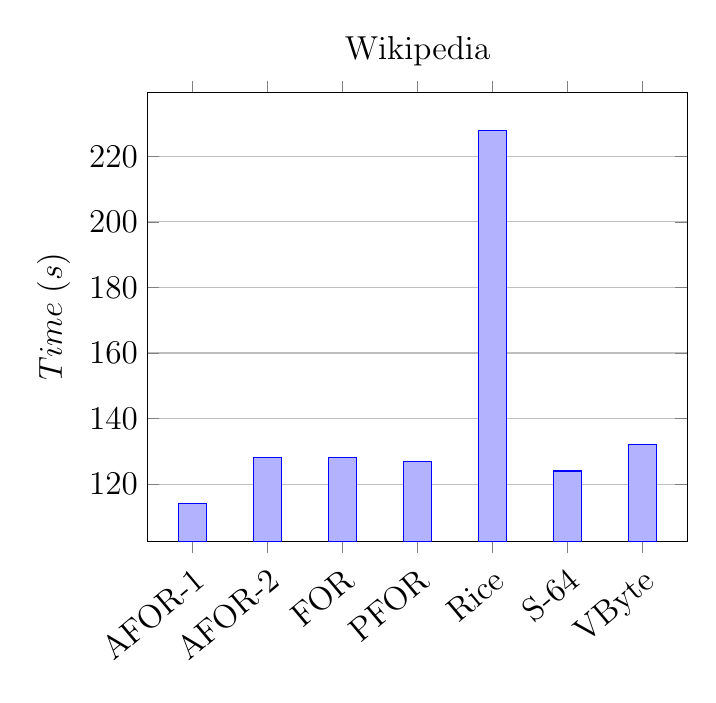
\begin{tikzpicture}[baseline]
\begin{axis}[
ylabel=$Time \; (s)$,
x tick label style={rotate=40, anchor=north east},
xtick={1,...,7},
xticklabels={AFOR-1, AFOR-2, FOR, PFOR, Rice, S-64, VByte},
legend style={at={(0.5,1.13)}, anchor=north, legend columns=-1},
label style={font=\large},
tick label style={font=\large},
title style={font=\large},
ybar,
ymajorgrids=true,
bar width=10pt,
title={Wikipedia},
%enlargelimits=0.15,
]
\addplot
coordinates {(1, 114) (2, 128) (3, 128) (4, 127) (5, 228) (6, 124) (7, 132)};
\end{axis}
\end{tikzpicture}%
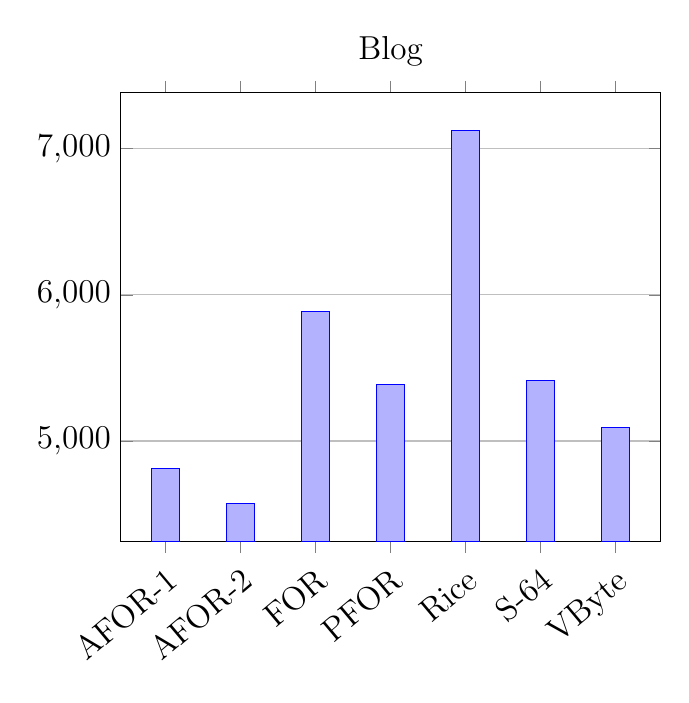
\begin{tikzpicture}[baseline]
\begin{axis}[
x tick label style={rotate=40, anchor=north east},
xtick={1,...,7},
xticklabels={AFOR-1, AFOR-2, FOR, PFOR, Rice, S-64, VByte},
legend style={at={(0.5,1.13)}, anchor=north, legend columns=-1},
label style={font=\large},
tick label style={font=\large},
title style={font=\large},
ybar,
ymajorgrids=true,
bar width=10pt,
title={Blog},
%enlargelimits=0.15,
]
\addplot
coordinates {(1, 4813) (2, 4571) (3, 5888) (4, 5387) (5, 7127) (6, 5414) (7,
5092)};
\end{axis}
\end{tikzpicture}
% }
  }
  \quad
  \resizebox{\linewidth}{!}{%
    % \subfloat[Structured data]{%
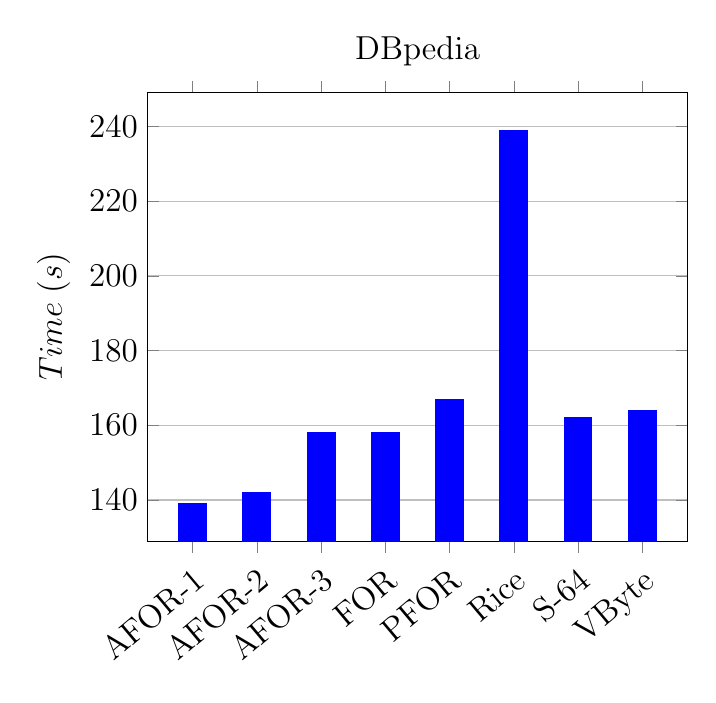
\begin{tikzpicture}[baseline]
\begin{axis}[
ylabel=$Time \; (s)$,
x tick label style={rotate=40, anchor=north east},
xtick={1,...,8},
xticklabels={AFOR-1, AFOR-2, AFOR-3, FOR, PFOR, Rice, S-64, VByte},
legend style={at={(0.5,1.13)}, anchor=north, legend columns=-1},
label style={font=\large},
tick label style={font=\large},
title style={font=\large},
ybar,
ymajorgrids=true,
bar width=10pt,
title={DBpedia},
%enlargelimits=0.15,
]
\addplot[draw=blue,fill=blue]
coordinates {(1, 139) (2, 142) (3, 158) (4, 158) (5, 167) (6, 239) (7, 162) (8, 164)};
\end{axis}
\end{tikzpicture}%
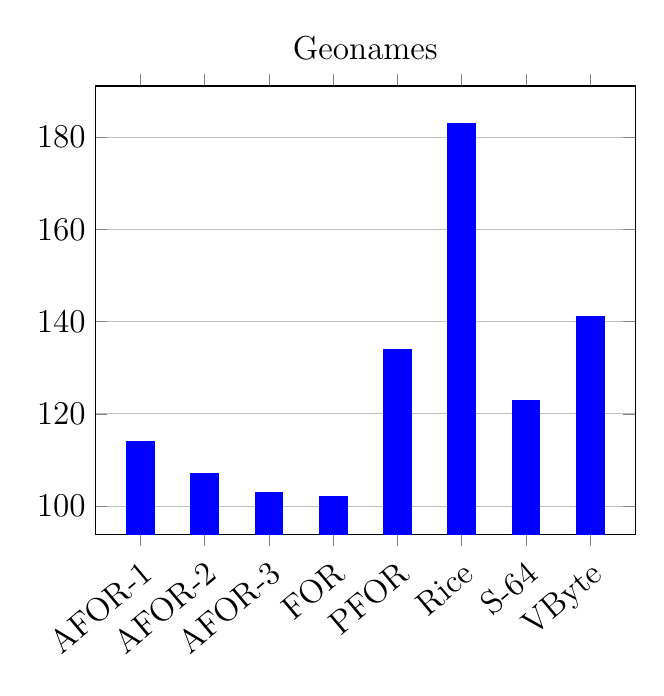
\begin{tikzpicture}[baseline]
\begin{axis}[
x tick label style={rotate=40, anchor=north east},
xtick={1,...,8},
xticklabels={AFOR-1, AFOR-2, AFOR-3, FOR, PFOR, Rice, S-64, VByte},
legend style={at={(0.5,1.13)}, anchor=north, legend columns=-1},
label style={font=\large},
tick label style={font=\large},
title style={font=\large},
ybar,
ymajorgrids=true,
bar width=10pt,
title={Geonames},
%enlargelimits=0.15,
]
\addplot[draw=blue,fill=blue]
coordinates {(1, 114) (2, 107) (3, 103) (4, 102) (5, 134) (6, 183) (7, 123) (8, 141)};
%\legend{Blog}
\end{axis}
\end{tikzpicture}
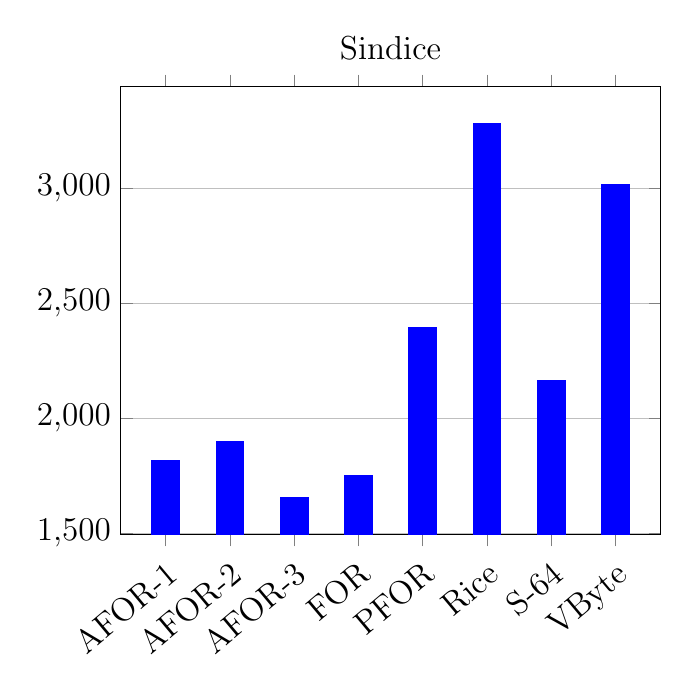
\begin{tikzpicture}[baseline]
\begin{axis}[
x tick label style={rotate=40, anchor=north east},
xtick={1,...,8},
xticklabels={AFOR-1, AFOR-2, AFOR-3, FOR, PFOR, Rice, S-64, VByte},
legend style={at={(0.5,1.13)}, anchor=north, legend columns=-1},
label style={font=\large},
tick label style={font=\large},
title style={font=\large},
ybar,
ymajorgrids=true,
bar width=10pt,
title={Sindice},
%enlargelimits=0.15,
]
\addplot[draw=blue,fill=blue]
coordinates {(1, 1816) (2, 1900) (3, 1656) (4, 1749) (5, 2396) (6, 3281) (7, 2163) (8, 3018)};
%\legend{Blog}
\end{axis}
\end{tikzpicture}
% }
  }
	\caption{The total time spent to optimise the complete index.}
	\label{fig:optimise-time}
\end{minipage}
\end{figure}

\paragraph{Compression Ratio}

Figure~\ref{fig:index-size} shows the total index size achieved by each
method. We can clearly see the inefficiency of the VByte approach. While VByte
performs generally better than FOR on traditional document-centric inverted
indexes like with Wikipedia and Blog datasets, this is not true for inverted
indexes based on a node indexing scheme like SIREn. VByte is not adapted to such
an index due to the properties of the delta-encoded lists of values. Apart
from the entity file, the values are generally very small and the outliers are
rare. In that case, VByte is penalized by its inability to encode a small
integer in less than a byte.

On the contrary, FOR is able to encode many small
integers in one byte. Also, while PFOR is less sensitive to outliers than FOR,
the gain of compression rate provided by PFOR is minimal since outliers are
more rare than in traditional inverted indexes. Indeed we can see that the
distribution of values with a document-centric indexing technique (Wikipedia
and Blog) lead to many outliers, and thus the PFOR algorithm is in that case
efficient.

In contrast, AFOR and S-64 are able to better adapt the encoding to
the value distribution and therefore provide a better compression rate. While
Rice provides the best compression ratio on traditional inverted indexes, AFOR
is able to provide better compression ratio than Rice on the Geonames and
Sindice dataset. Compared to AFOR-2, we can observe in
Table~\ref{tab:indexing-performance} that AFOR-3 provides better compression
rate on the frequency, value and position files, and slightly better on the
entity file. This result corroborates the existence of long runs of 1 in these
files, as explained in Section~\ref{sec:compression:stripping}.

In comparison to normal indexes, Rice provides worse compression ratio than
AFOR on a node indexing scheme index. This can be explained again by the small
values, since Rice does not compress long runs of small values as well as AFOR.

\begin{figure}
\centering
\begin{minipage}{0.8\linewidth}
  \centering
    \resizebox{0.7\linewidth}{!}{%
    % \subfloat[Unstructured data]{%
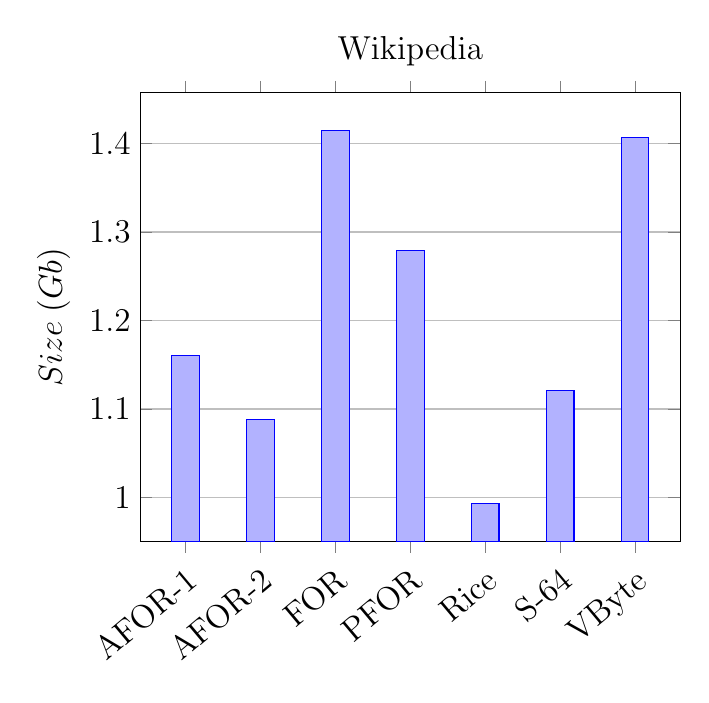
\begin{tikzpicture}[baseline]
\begin{axis}[
ylabel=$Size \; (Gb)$,
x tick label style={rotate=40, anchor=north east},
xtick={1,...,7},
xticklabels={AFOR-1, AFOR-2, FOR, PFOR, Rice, S-64, VByte},
legend style={at={(0.5,1.13)}, anchor=north, legend columns=-1},
label style={font=\large},
tick label style={font=\large},
title style={font=\large},
ybar,
ymajorgrids=true,
bar width=10pt,
title={Wikipedia},
%enlargelimits=0.15,
]
\addplot
coordinates {(1, 1.160) (2, 1.088) (3, 1.415) (4, 1.279) (5, 0.993) (6, 1.121)
(7, 1.407)};
\end{axis}
\end{tikzpicture}%

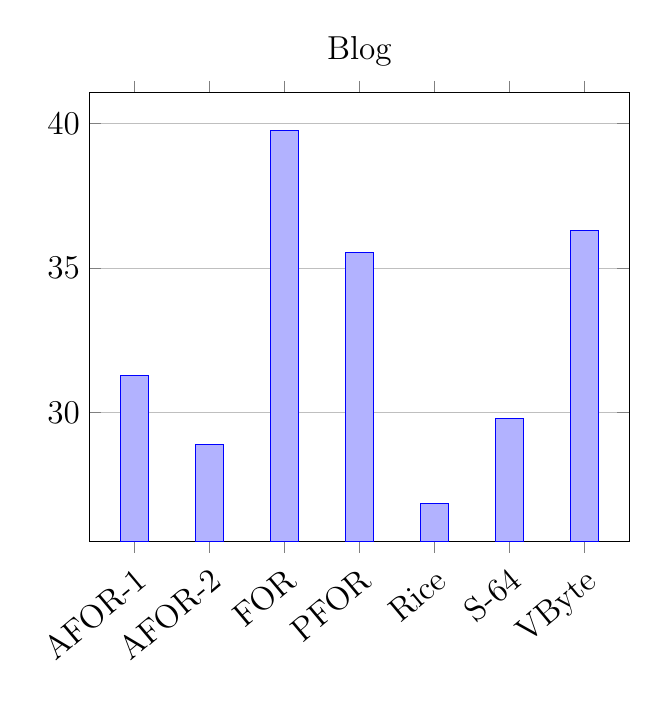
\begin{tikzpicture}[baseline]
\begin{axis}[
x tick label style={rotate=40, anchor=north east},
xtick={1,...,7},
xticklabels={AFOR-1, AFOR-2, FOR, PFOR, Rice, S-64, VByte},
legend style={at={(0.5,1.13)}, anchor=north, legend columns=-1},
label style={font=\large},
tick label style={font=\large},
title style={font=\large},
ybar,
ymajorgrids=true,
bar width=10pt,
title={Blog},
%enlargelimits=0.15,
]
\addplot
coordinates {(1, 31.292) (2, 28.895) (3, 39.777) (4, 35.536) (5, 26.851) (6,
29.800) (7, 36.303)};
\end{axis}
\end{tikzpicture}%
% }
  }
  \quad
  \resizebox{\linewidth}{!}{%
    % \subfloat[Unstructured data]{%
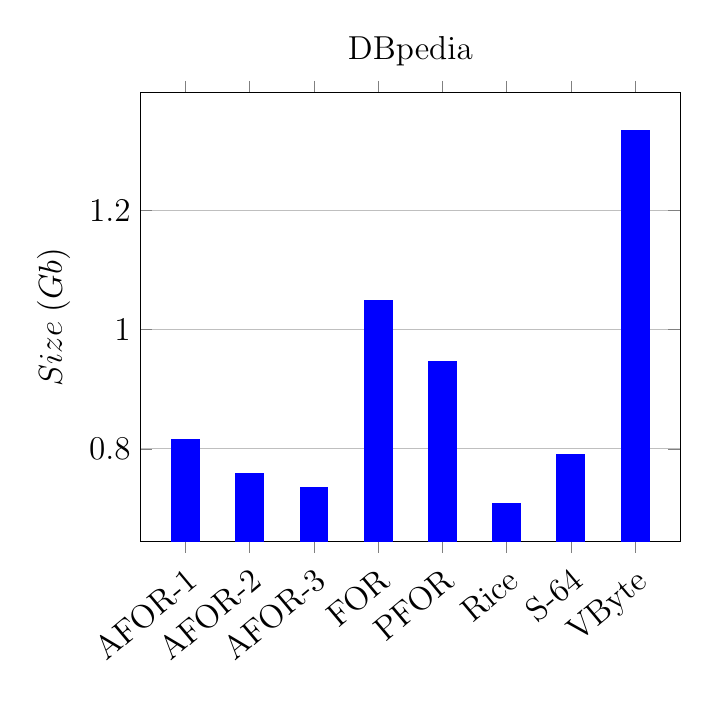
\begin{tikzpicture}[baseline]
\begin{axis}[
ylabel=$Size \; (Gb)$,
x tick label style={rotate=40, anchor=north east},
xtick={1,...,8},
xticklabels={AFOR-1, AFOR-2, AFOR-3, FOR, PFOR, Rice, S-64, VByte},
legend style={at={(0.5,1.13)}, anchor=north, legend columns=-1},
label style={font=\large},
tick label style={font=\large},
title style={font=\large},
ybar,
ymajorgrids=true,
bar width=10pt,
title={DBpedia},
%enlargelimits=0.15,
]
\addplot[draw=blue,fill=blue]
coordinates {(1, 0.816) (2, 0.758) (3, 0.736) (4, 1.049) (5, 0.946) (6, 0.708) (7, 0.791) (8, 1.335)};
\end{axis}
\end{tikzpicture}%
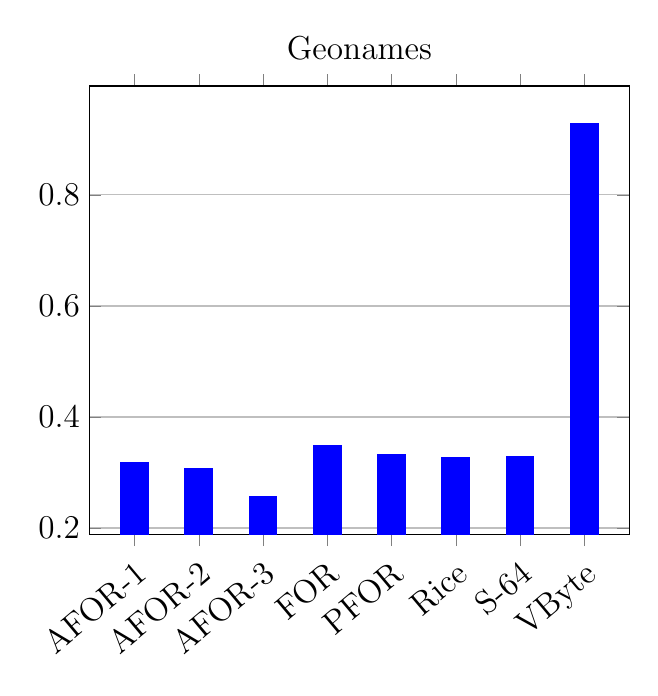
\begin{tikzpicture}[baseline]
\begin{axis}[
x tick label style={rotate=40, anchor=north east},
xtick={1,...,8},
xticklabels={AFOR-1, AFOR-2, AFOR-3, FOR, PFOR, Rice, S-64, VByte},
legend style={at={(0.5,1.13)}, anchor=north, legend columns=-1},
label style={font=\large},
tick label style={font=\large},
title style={font=\large},
ybar,
ymajorgrids=true,
bar width=10pt,
title={Geonames},
%enlargelimits=0.15,
]
\addplot[draw=blue,fill=blue]
coordinates {(1, 0.318) (2, 0.307) (3, 0.256) (4, 0.349) (5, 0.332) (6, 0.327) (7, 0.329) (8, 0.929)};
\end{axis}
\end{tikzpicture}%
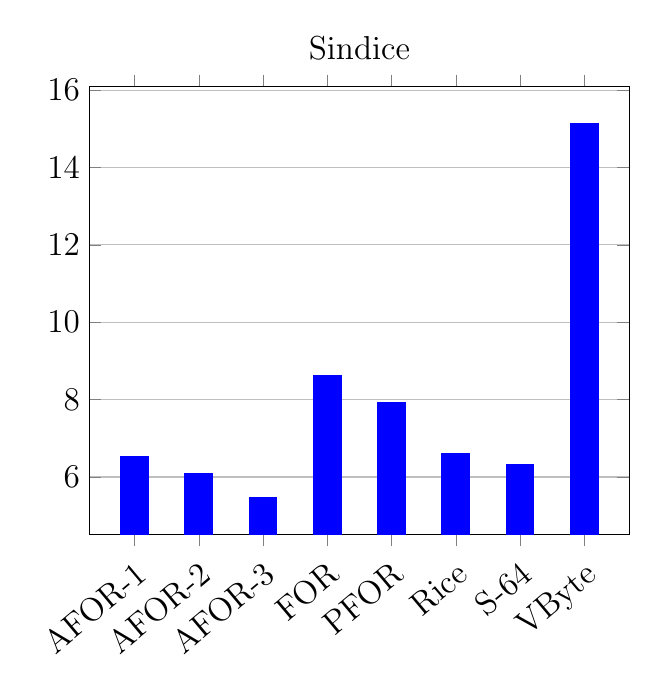
\begin{tikzpicture}[baseline]
\begin{axis}[
x tick label style={rotate=40, anchor=north east},
xtick={1,...,8},
xticklabels={AFOR-1, AFOR-2, AFOR-3, FOR, PFOR, Rice, S-64, VByte},
legend style={at={(0.5,1.13)}, anchor=north, legend columns=-1},
label style={font=\large},
tick label style={font=\large},
title style={font=\large},
ybar,
ymajorgrids=true,
bar width=10pt,
title={Sindice},
%enlargelimits=0.15,
]
\addplot[draw=blue,fill=blue]
coordinates {(1, 6.537) (2, 6.082) (3, 5.475) (4, 8.611) (5, 7.924) (6, 6.605) (7, 6.313) (8, 15.132)};
\end{axis}
\end{tikzpicture}%
% }
  }
	\caption{The index size achieved by each compression technique.}
	\label{fig:index-size}
\end{minipage}
\end{figure}

\paragraph{Conclusion on Indexing Performance}

The indexing experiment shows that the compression speed is also an important
factor to take into consideration when designing a compression algorithm for
an inverted index. Without a good compression speed, the update throughput of
the index is limited. Also the experiment shows that the optimisation
operation is dependent of the decompression performance, and its execution
time can double without a good compression and decompression speed. With
respect to index optimisation, the compression ratio must also be taken into
consideration. While VByte provides in general correct commit times, we can
observe on a large dataset (Sindice) that its performance during optimisation
is limited by its poor compression ratio.

Overall, the method providing the best balance between indexing time, optimise
time and compression ratio is the AFOR family, and this on both structured and
unstructured datasets. AFOR-1 provides fast compression speed and better
compression ratio than FOR and PFOR. AFOR-2 provides a notable additional gain
in compression ratio and optimise time but undergoes a slight increase of
indexing time. AFOR-3 provides another additional gain in compression ratio
while providing better compression speed than AFOR-2.

\section{Querying Performance}
\label{sec:compression:query-performance}

We now compare the decompression performance in real settings, where inverted
indexes are answering queries of various complexities. We report in this
section only the benchmarks done on structured datasets (DBpedia,
Geonames and Sindice), since the performance of query processing on unstructured
datasets is comparable to the ones run on the structured datasets and for
question of clarity also. The raw results are nonetheless reported in the
appendix in the Table~\ref{tab:query-time-TRAD}.

We focus on two main classes of queries, the value and attribute queries, which
are the core elements of a star-shaped query. Among these two classes, we
identify types of keyword queries which represent the common queries received
by a web search engine: conjunction, disjunction and phrase.

\subsection{Query Benchmarking Framework}
\label{sec:bench-query-FW}

In this section we present the types of queries that are run against indexes
compressed with different algorithms.

\subsection{Query Generation}

The queries are generated based on the selectivity of the words composing
them. The word selectivity determines how many entities match a given keyword.
The words are grouped into three selectivity ranges: \emph{high}, \emph{medium}
and \emph{low}. We differentiate also two groups of
words based on their position in the data graph: attribute and value. We
follow the technique described in \cite{errcegovac:2005:vldb} to obtain the
ranges of each word group. We first order the words by their descending
frequency, and then take the first $k$ words whose cumulative frequency is
90\% of all word occurrences as high range. The medium range accounts for the
next 10\%, and the low range is composed of all the remaining words. For the
phrase queries, we follow a similar technique. We first extract all the 2-gram
and 3-gram\footnote{A n-gram is $n$ words that appear contiguously} from the
data collection. We then compute their frequency and sort them by descending
frequency. We finally create the three ranges as explained above. Benchmarks
involving queries with words from low and medium ranges are not reported here
for questions of space, but the performance results are comparable with the
one presented here.

\subsubsection{Value Queries}

Value queries are divided into three types of keyword queries:
\emph{conjunction}, \emph{disjunction} and \emph{phrase} queries. These queries
are restricted to match within one single value, e.g. to find all entities
which have the word ``fantasy'' within a value as in \ref{fig:entities}.
Therefore, the processing of conjunction and disjunction queries relies on the
entity, frequency, attribute and value inverted files. Phrase queries rely on
one additional stream, the position values.

Conjunction and disjunction queries are generated by taking random keywords
from the high range group of words. 2-AND and 2-OR (resp. 4-AND and 4-OR)
denotes conjunction and disjunction queries with 2 random keywords (resp. 4
random keywords). Similarly, a phrase query is generated by taking random
n-grams from the high range group. 2-Phrase (resp. 3-Phrase) denotes phrase
queries with 2-gram (resp. 3-gram). Benchmarks involving queries with words
from low and medium ranges are not reported here for questions of space, but
the performance results are comparable with the ones presented here.

\subsubsection{Attribute Queries}

An attribute query is generated by associating one attribute keyword with one
value query. An attribute keyword is randomly chosen from the high range
groups of attribute words. The associated value query is obtained as explained
previously. An attribute query intersects the result of a value query with an
attribute keyword.

\subsection{Query Benchmark Design}

The benchmarking design used is the one presented in the
Chapter~\ref{chap:benchmarking-framework}. For each type of query, we 
\begin{inparaenum}[(1)]
\item generate a set of 200 random queries which is reused for all the
compression methods, and
\item perform 100 measurements.
\end{inparaenum}
All measurements are made using \emph{warm cache}, i.e., the part of the index
read during query processing is fully loaded in memory.

Query execution time is sensitive to external events which can affect the
final execution time recorded.
% For instance, background system maintenance or
% interruptions as well as cache misses or system exceptions can occur and
% perturb the measurements. All these events are unpredictable and must be
% treated as noise. Therefore, we need to quantify the accuracy of our
% measurements.
% As recommended in \cite{lilja:2000:book}, we report the
% arithmetic mean and the standard deviation of the 100 measurements.
To assess differences between the algorithms, confidence intervals with 95\%
degree of confidence have been used.  The design of the value and attribute
query benchmarks includes three factors:
\begin{description}
\item[Algorithm] having height levels: AFOR-1, AFOR-2, AFOR-3, FOR, PFOR,
Rice, S-64, and VByte;
\item[Query] having six levels: 2-AND, 2-OR, 4-AND, 4-OR, 2-Phrase, and
3-Phrase; and
\item[Dataset] having three levels: DBpedia, Geonames and Sindice. 
\end{description}
Each condition of the design, e.g., AFOR-1 / 2-AND / DBpedia, contains 100
separate measurements.

\subsection{Query Benchmark Results}

We report the results of the query benchmarks in
Table~\ref{tab:value-query-time} and Table~\ref{tab:attribute-query-time} in
the appendix for the value and attribute queries respectively. Based on these
results, we derive multiple graphical charts to better visualise the
differences between each algorithm. These charts are then used to compare and
discuss the performances of each algorithm.

Figure~\ref{fig:avg-value-query-time} and
Figure~\ref{fig:avg-attribute-query-time} report the average query processing
time for the value and attribute queries respectively.
Figure~\ref{fig:avg-value-boolean-query-time} and
Figure~\ref{fig:avg-attribute-boolean-query-time} depict the average
processing time on the Boolean queries.
Figure~\ref{fig:avg-value-phrase-query-time} and
Figure~\ref{fig:avg-attribute-phrase-query-time} depict the average processing
time on the phrase queries (2-Phrase, 3-Phrase). The query processing time are
obtained by summing up the average time of each query from
Table~\ref{tab:value-query-time} for the value queries and
Table~\ref{tab:attribute-query-time} for the attribute queries. For example,
the processing time of AFOR-1 on the DBpedia dataset in
Figure~\ref{fig:avg-value-phrase-query-time} is obtained by summing up the
processing times of the queries 2-Phrase (43.2 ms) and 3-Phrase (32.6 ms)
reported in Table~\ref{tab:value-query-time} in the appendix.

\paragraph{Value Query}

In Figure~\ref{fig:avg-value-query-time}, and in particular on the Sindice
dataset (large dataset), we can distinguish three classes of algorithms: the
techniques based on FOR, a group composed of S-64 and VByte, and finally Rice.
The FOR group achieves relatively similar results, with AFOR-2 slightly behind
the others.

Rice has the worst performance for every query and dataset, followed by VByte.
Nonetheless Rice performs in many cases twice as slow as VByte. In
Figure~\ref{fig:avg-value-boolean-query-time}, S-64 provides similar
performance to VByte on Boolean queries but we can see in
Figure~\ref{fig:avg-value-phrase-query-time} that it is faster than VByte on
phrase queries. However, S-64 stays behind FOR, PFOR and AFOR in all the cases.

FOR, PFOR and AFOR have relatively similar performances on all the Boolean
queries and all the datasets. PFOR seems to provide generally slightly better
performance on the phrase queries but seems to be slower on Boolean queries.

\begin{figure}
  \centering
  \subfloat[Boolean Query]{%
    \resizebox{0.45\linewidth}{!}{%
      
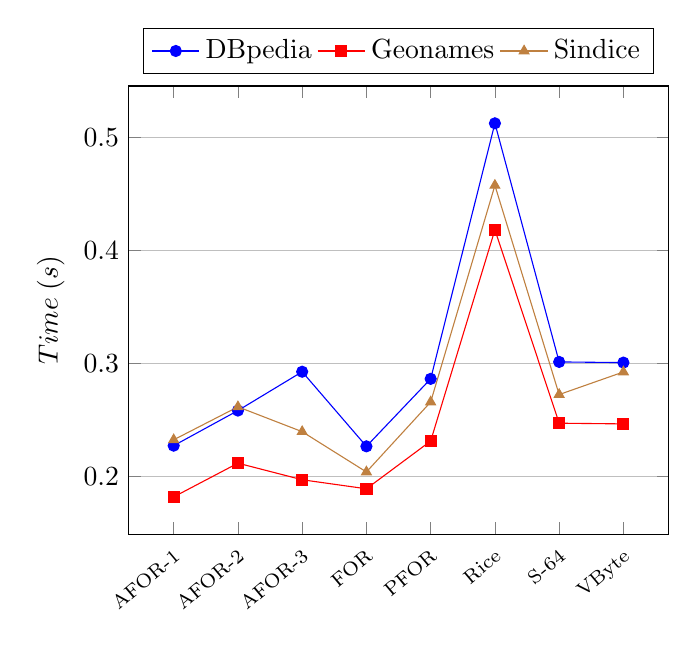
\begin{tikzpicture}
\begin{axis}[
ylabel=$Time \; (s)$,
x tick label style={font=\scriptsize, rotate=40, anchor=north east},
xtick={1,...,8},
xticklabels={AFOR-1, AFOR-2, AFOR-3, FOR, PFOR, Rice, S-64, VByte},
legend style={at={(0.5,1.13)}, anchor=north, legend columns=-1},
%ybar,
ymajorgrids=true,
%bar width=5pt,
]

\addplot[blue,mark=*]
coordinates {(1, 0.2271) (2, 0.2582) (3, 0.2926) (4, 0.2265) (5, 0.2863) (6, 0.5127) (7, 0.3013) (8, 0.3007)};
\addplot[red,mark=square*]
coordinates {(1, 0.1817) (2, 0.2116) (3, 0.1969) (4, 0.1889) (5, 0.2312) (6, 0.4184) (7, 0.2470) (8, 0.2464)};
\addplot[brown,mark=triangle*]
coordinates {(1, 0.2323) (2, 0.2615) (3, 0.2395) (4, 0.2038) (5, 0.2658) (6, 0.4577) (7, 0.2724) (8, 0.2924)};

\legend{DBpedia, Geonames, Sindice}

\end{axis}
\end{tikzpicture}%

  	}
  	\label{fig:avg-value-boolean-query-time}
  }\quad%
  \subfloat[Phrase Query]{%
    \resizebox{0.45\linewidth}{!}{%
      
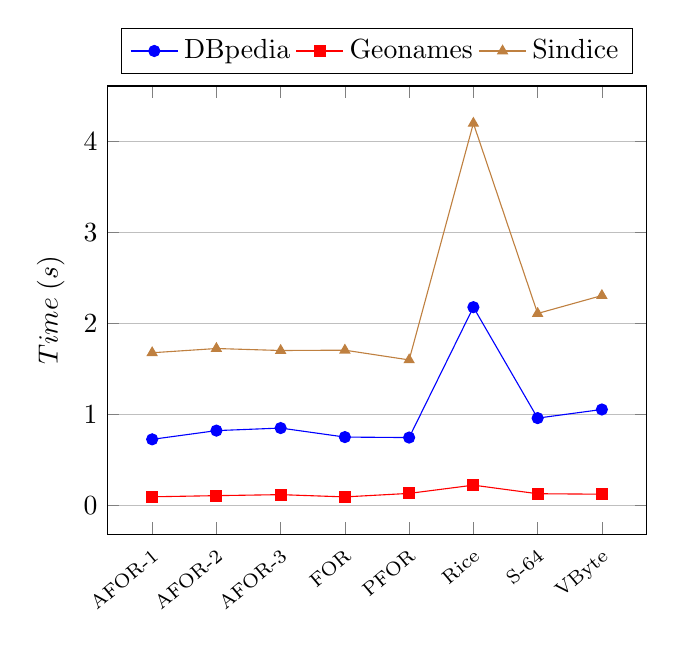
\begin{tikzpicture}
\begin{axis}[
ylabel=$Time \; (s)$,
x tick label style={font=\scriptsize, rotate=40, anchor=north east},
xtick={1,...,8},
xticklabels={AFOR-1, AFOR-2, AFOR-3, FOR, PFOR, Rice, S-64, VByte},
legend style={at={(0.5,1.13)}, anchor=north, legend columns=-1},
%ybar,
ymajorgrids=true,
%bar width=5pt,
]

\addplot[blue,mark=*]
coordinates {(1, 0.7267) (2, 0.8225) (3, 0.8506) (4, 0.7516) (5, 0.7462) (6, 2.1778) (7, 0.9598) (8, 1.0544) };
\addplot[red,mark=square*]
coordinates {(1, 0.0959) (2, 0.1085) (3, 0.1196) (4, 0.0947) (5, 0.1333) (6, 0.2237) (7, 0.1296) (8, 0.1245)};
\addplot[brown,mark=triangle*]
coordinates {(1, 1.6773) (2, 1.7239) (3, 1.702) (4, 1.7056) (5, 1.5986) (6, 4.1963) (7, 2.1086) (8, 2.3053)};

\legend{DBpedia, Geonames, Sindice}

\end{axis}
\end{tikzpicture}%

    }
    \label{fig:avg-value-phrase-query-time}
  }%
	\caption{The average processing time for the value queries that is achieved
	by each compression technique.}
	\label{fig:avg-value-query-time}
\end{figure}

\paragraph{Attribute Query}

In Figure~\ref{fig:avg-attribute-query-time}, and in particular on Sindice, we
can again distinguish the same three classes of algorithms. However, the
performance gap between S-64 and VByte becomes wider.

Rice has again the worst performance for every query and dataset. Compared to
the performance on value queries, we can see in
Figure~\ref{fig:avg-attribute-boolean-query-time} that S-64 provides similar
performance to PFOR and AFOR-2 on Boolean queries. FOR and AFOR-3 seem to be
the best performing methods on Boolean queries. With respect to the phrase
queries in Figure~\ref{fig:avg-attribute-phrase-query-time}, S-64 has better
performance than VByte. However, PFOR does not achieve any more the best
performance on phrase queries. Instead, it seems that AFOR-2 and FOR achieve a
slightly better processing time.

FOR, PFOR and AFOR have again relatively similar performances on all the
queries and all the datasets. AFOR-2 appears to be slower to some degree,
while the gap between AFOR-3 and PFOR becomes less perceptible.

\begin{figure}
  \centering
  \subfloat[Boolean Query]{%
    \resizebox{0.45\linewidth}{!}{%
      
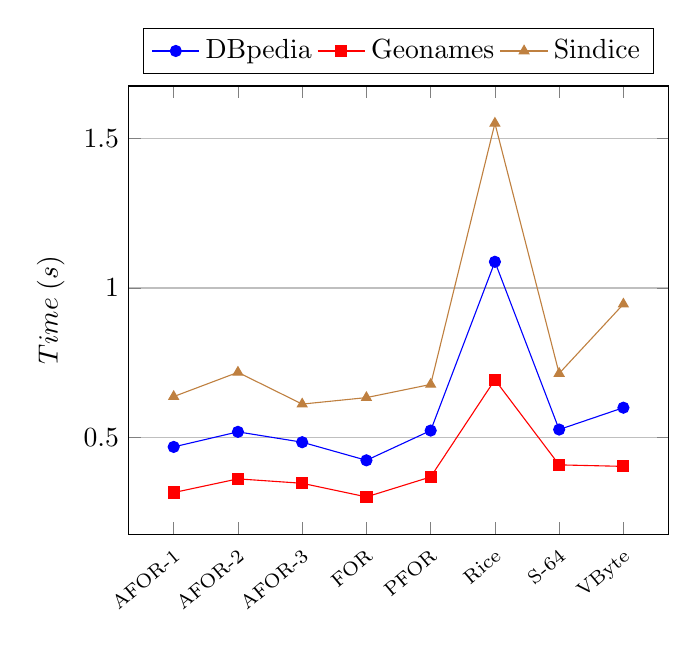
\begin{tikzpicture}
\begin{axis}[
ylabel=$Time \; (s)$,
x tick label style={font=\scriptsize, rotate=40, anchor=north east},
xtick={1,...,8},
xticklabels={AFOR-1, AFOR-2, AFOR-3, FOR, PFOR, Rice, S-64, VByte},
legend style={at={(0.5,1.13)}, anchor=north, legend columns=-1},
%ybar,
ymajorgrids=true,
%bar width=7pt,
]

\addplot[blue,mark=*]
coordinates {(1, 0.4692) (2, 0.5195) (3, 0.4849) (4, 0.4244) (5, 0.5238) (6, 1.0875) (7, 0.5272) (8, 0.6002)};
\addplot[red,mark=square*]
coordinates {(1, 0.3167) (2, 0.3625) (3, 0.3477) (4, 0.3022) (5, 0.3689) (6, 0.6936) (7, 0.4092) (8, 0.4042)};
\addplot[brown,mark=triangle*]
coordinates {(1, 0.6373) (2, 0.7183) (3, 0.6122) (4, 0.6339) (5, 0.6779) (6, 1.55) (7, 0.7146) (8, 0.946)};

\legend{DBpedia, Geonames, Sindice}

\end{axis}
\end{tikzpicture}


  	}
  	\label{fig:avg-attribute-boolean-query-time}
  }\quad%
  \subfloat[Phrase Query]{%
    \resizebox{0.45\linewidth}{!}{%
      
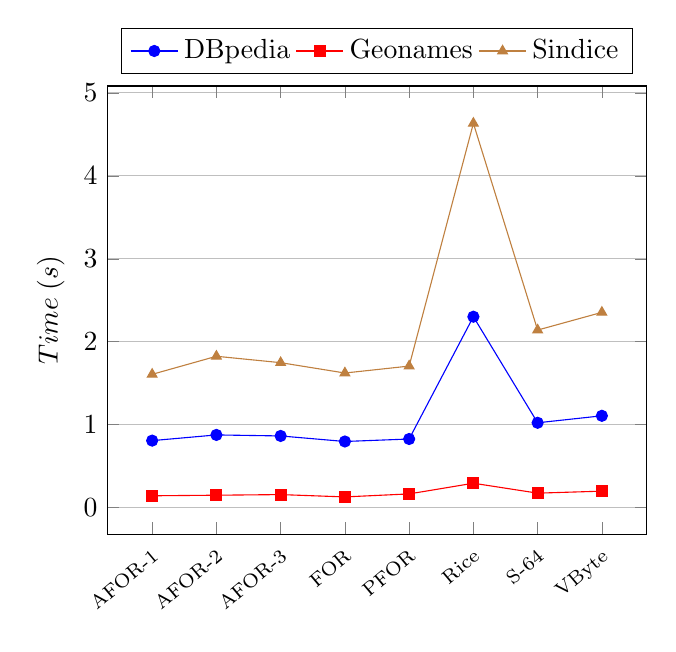
\begin{tikzpicture}
\begin{axis}[
ylabel=$Time \; (s)$,
x tick label style={font=\scriptsize, rotate=40, anchor=north east},
xtick={1,...,8},
xticklabels={AFOR-1, AFOR-2, AFOR-3, FOR, PFOR, Rice, S-64, VByte},
legend style={at={(0.5,1.13)}, anchor=north, legend columns=-1},
%ybar,
ymajorgrids=true,
%bar width=7pt,
]

\addplot[blue,mark=*]
coordinates {(1, 0.8081) (2, 0.8767) (3, 0.8644) (4, 0.7976) (5, 0.8275) (6, 2.302) (7, 1.0232) (8, 1.1072)};
\addplot[red,mark=square*]
coordinates {(1, 0.143) (2, 0.1499) (3, 0.1574) (4, 0.1293) (5, 0.1656) (6, 0.2943) (7, 0.1747) (8, 0.1988)};
\addplot[brown,mark=triangle*]
coordinates {(1, 1.6073) (2, 1.825) (3, 1.7478) (4, 1.6231) (5, 1.7067) (6, 4.6336) (7, 2.1409) (8, 2.3544)};

\legend{DBpedia, Geonames, Sindice}

\end{axis}
\end{tikzpicture}


    }
    \label{fig:avg-attribute-phrase-query-time}
  }%
	\caption{The average processing time for the attribute queries that is
	achieved by each compression technique.}
	\label{fig:avg-attribute-query-time}
\end{figure}

\section{Performance Trade-Off}

We report in Figure~\ref{fig:trade-off-time-bytes} the trade-off between the
total query processing time and the compression ratio among all the techniques
on the Sindice dataset. The total query time has been obtained by summing up
the average time of all the queries. The compression ratio is based on the
number of bytes read during query processing which are reported in
Table~\ref{tab:value-query-time} and Table~\ref{tab:attribute-query-time} in
the appendix.
We can distinctively see that the AFOR techniques are close to Rice in term of
compression ratio, while being relatively close to FOR and PFOR in term of
query processing time. Compared to AFOR-1, AFOR-2 achieves a better
compression rate in exchange of a slightly slower processing time. However,
AFOR-3 accomplishes a better compression rate with a processing time close to
AFOR-1.

\begin{figure}
  \centering
  \subfloat[Value Query]{%
    \resizebox{0.47\linewidth}{!}{%
      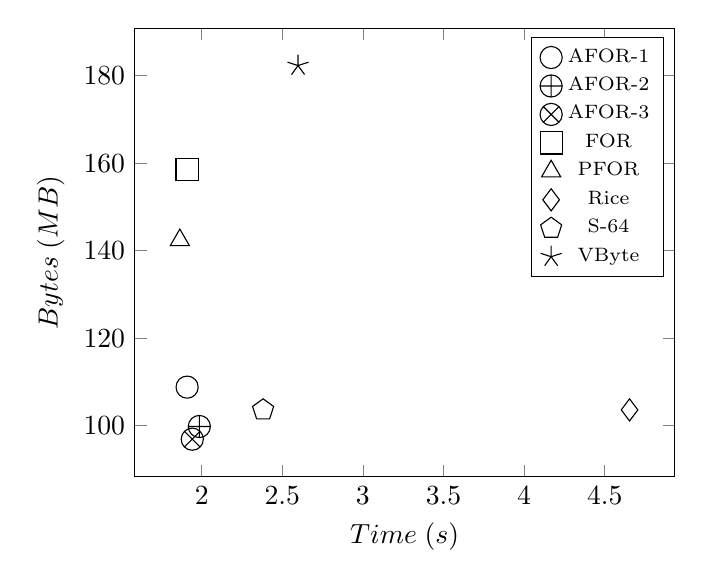
\begin{tikzpicture}
\begin{axis}[
scatter/classes={
	a={mark=o},
	b={mark=oplus},
	c={mark=otimes},
	d={mark=square},
	e={mark=triangle},
	f={mark=diamond},
	g={mark=pentagon},
	h={mark=star}
  },
  ylabel=$Bytes \; (MB)$,
  xlabel=$Time \; (s)$,
  mark options={scale=2},
  legend style={font=\scriptsize}
]

\addplot[scatter, only marks]
plot[scatter src=explicit symbolic]
coordinates {
(1.9096, 108.8) [a]
(1.9854, 99.8) [b]
(1.9415, 96.9) [c]
(1.9094, 158.5) [d]
(1.8644, 142.4) [e]
(4.654, 103.6) [f]
(2.381, 103.6) [g]
(2.5977, 182.3) [h]
};

\legend{AFOR-1, AFOR-2, AFOR-3, FOR, PFOR, Rice, S-64, VByte}

\end{axis}
\end{tikzpicture}
  	}
  }%
  \subfloat[Attribute Query]{%
    \resizebox{0.47\linewidth}{!}{%
      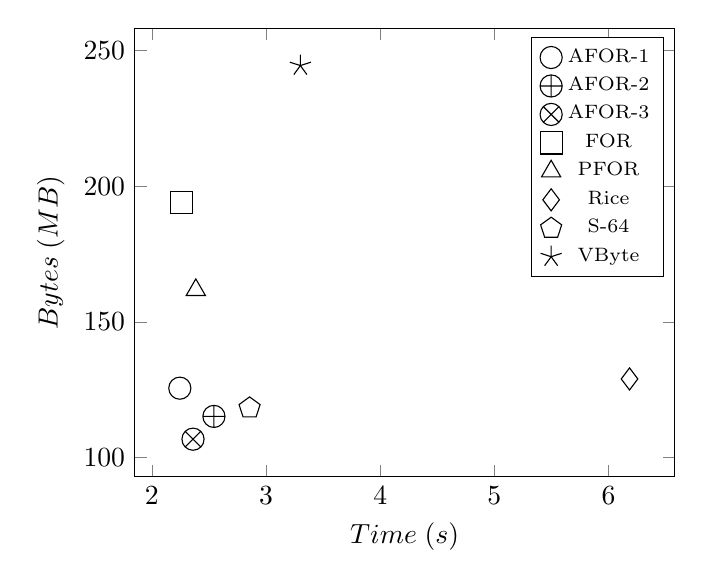
\begin{tikzpicture}
\begin{axis}[
	scatter/classes={
	a={mark=o},
	b={mark=oplus},
	c={mark=otimes},
	d={mark=square},
	e={mark=triangle},
	f={mark=diamond},
	g={mark=pentagon},
	h={mark=star}
  },
  ylabel=$Bytes \; (MB)$,
  xlabel=$Time \; (s)$,
  mark options={scale=2},
  legend style={font=\scriptsize},
]

\addplot[only marks]
plot[scatter, scatter src=explicit symbolic]
coordinates {
 (2.2446, 125.6) [a]
 (2.5433, 115.2) [b]
 (2.36, 106.8) [c]
 (2.257, 194.0) [d]
 (2.3846, 161.8) [e]
 (6.1836, 129.0) [f]
 (2.8555, 118.3) [g]
 (3.3004, 244.5) [h]
};
\legend{AFOR-1, AFOR-2, AFOR-3, FOR, PFOR, Rice, S-64, VByte}
\end{axis}
\end{tikzpicture}
    }
  }%
	\caption{A graphical comparison showing the trade-off between querying time
	and compression ratio on the Sindice dataset. The compression ratio is
	represented by the number of bytes read during the query processing.}
	\label{fig:trade-off-time-bytes}
\end{figure}

We report in Figure~\ref{fig:trade-off-query-update} the trade-off between the
total query processing time and the indexing time among all the techniques on
the Sindice dataset. The indexing time has been obtained by summing up the
commit and optimise time from Table~\ref{tab:indexing-performance} of the
appendix. We can distinctively see that the AFOR techniques achieve the best
trade-off between indexing and querying time. AFOR-3 produce very similar
indexing and querying times to AFOR-1, while providing a much better
compression rate. It is interesting to notice that PFOR provides a slightly
better querying time than FOR but at the price of a much slower compression.
Also, S-64 and VByte provide a relatively close performance trade-off. To
conclude, AFOR-3 seems to offer the best compromise between querying time,
indexing time, and compression rate.

\begin{figure}
  \centering
  \subfloat[Value Query]{%
    \resizebox{0.47\linewidth}{!}{%
      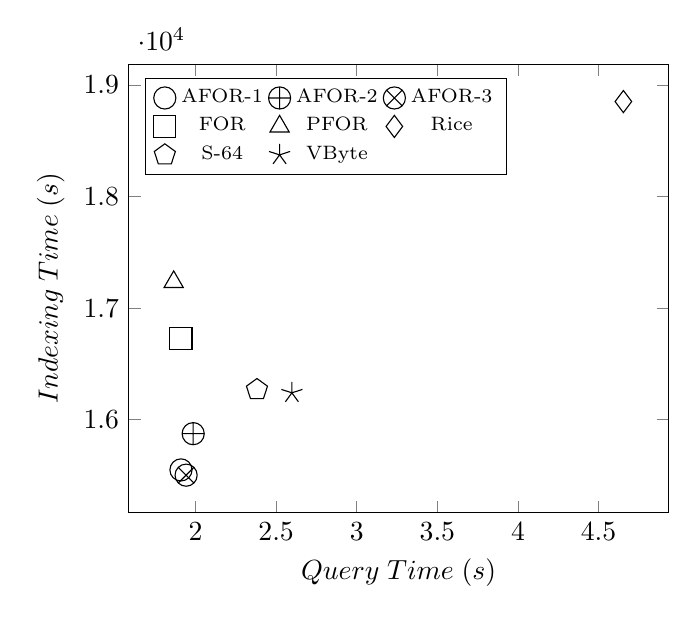
\begin{tikzpicture}
\begin{axis}[%
  scatter/classes={%
	a={mark=o},%
	b={mark=oplus},%
	c={mark=otimes},%
	d={mark=square},%
	e={mark=triangle},%
	f={mark=diamond},%
	g={mark=pentagon},%
	h={mark=star}
  },
  ylabel=$Indexing \; Time \; (s)$,
  xlabel=$Query \; Time \; (s)$,
  mark options={scale=2},
  legend columns=3,
  legend pos=north west,
  legend style={font=\scriptsize, anchor=north west, legend columns=3},
]

\addplot[only marks]
plot[scatter,scatter src=explicit symbolic]
coordinates {%
(1.9096, 15550) [a]
(1.9854, 15875) [b]
(1.9415, 15503) [c]
(1.9094, 16727) [d]
(1.8644, 17235) [e]
(4.654, 18852) [f]
(2.381, 16270) [g]
(2.5977, 16241) [h]
};%
\legend{AFOR-1, AFOR-2, AFOR-3, FOR, PFOR, Rice, S-64, VByte}
\end{axis}
\end{tikzpicture}
  	}
  }%
  \subfloat[Attribute Query]{%
    \resizebox{0.47\linewidth}{!}{%
      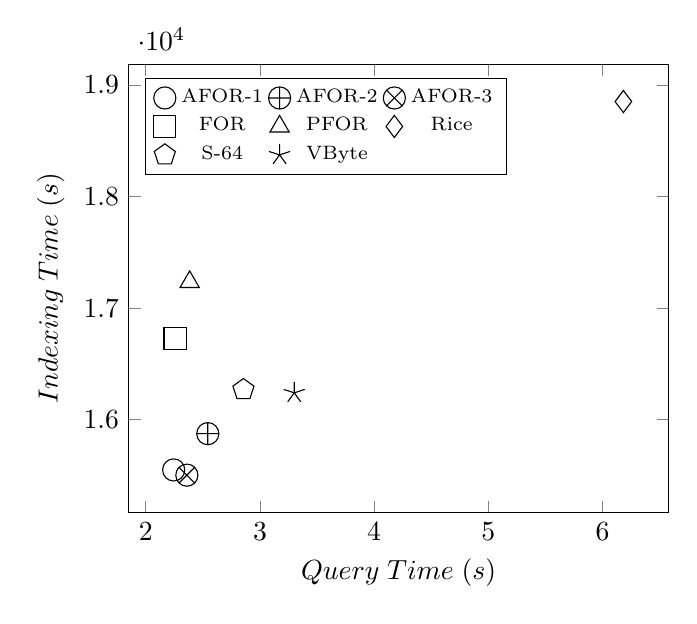
\begin{tikzpicture}
\begin{axis}[
  scatter/classes={
	a={mark=o},%
	b={mark=oplus},%
	c={mark=otimes},%
	d={mark=square},%
	e={mark=triangle},%
	f={mark=diamond},%
	g={mark=pentagon},%
	h={mark=star}
  },
  ylabel=$Indexing \; Time \; (s)$,
  xlabel=$Query \; Time \; (s)$,
  mark options={scale=2},
  legend columns=3,
  legend pos=north west,
  legend style={font=\scriptsize, anchor=north west, legend columns=3}
]

\addplot[only marks]
plot[scatter,mark=*,scatter src=explicit symbolic]
coordinates {
(2.2446, 15550) [a]
(2.5433, 15875) [b]
(2.3600, 15503) [c]
(2.2570, 16727) [d]
(2.3846, 17235) [e]
(6.1836, 18852) [f]
(2.8555, 16270) [g]
(3.3004, 16241) [h]
};
\legend{AFOR-1, AFOR-2, AFOR-3, FOR, PFOR, Rice, S-64, VByte}
\end{axis}
\end{tikzpicture}
    }
  }%
\caption{A graphical comparison of the compression techniques showing the
trade-off between querying time and indexing time on the Sindice dataset.}
\label{fig:trade-off-query-update}
\end{figure}

\section{Discussion}

In general, even if FOR has more data to read and decompress, it still
provides one of the best query execution time. The reason is that our
experiments are performed using warm cache. We therefore ignore the cost of
disk IO accesses and measure exclusively the decompression efficiency of the
methods. With a cold cache, i.e., when IO disk accesses have to be performed,
we expect a drop of performance for algorithms with a low compression ratio
such as FOR and PFOR compared to AFOR-2 and AFOR-3.

Compression and decompression performance do not only depend on the
compression ratio, but also on the execution flow of the algorithm and on the
number of cycles needed to compress or decompress an integer. Therefore,
CPU-optimised algorithms which provides at the same time a good compression
ratio are most likely to increase the update and query throughput of web
search engines. In that context, AFOR seems to be a good candidate since it is
well balanced in all aspects: it provides very good indexing and querying
performance and one of the best compression ratio.

The Simple encoding family is somehow similar to AFOR. At each iteration, S-64
encodes or decodes a variable number of integers using CPU optimised routines.
AFOR is however not tied to the size of a machine word, and is thus simpler to
implement and provides better compression ratio, compression speed and
decompression speed.


\chapter{Scalability of SIREn}{
In the previous experiments, we have seen that AFOR-3 is the most suitable
compression technique for an entity inverted index like SIREn. Based on these
results, we perform a stress test of the entity index compressed with AFOR-3
through a large scale experiment which simulates the conditions of a real Web
Data search engine such as Sindice. We use the full Sindice data collection to
create three indexes of increasing size and we generate a set of star queries
of increasing complexity. We compare the query rate (queries per second)
the system can answer with respect to the size of the index and the complexity
of the query.
}
\label{chap:scalability}
\section{Benchmarking Framework}

In this section we discuss the ability of the AFOR compression techniques
family to scale with the growing size of the compressed data.

\paragraph{Data Collection}

The full Sindice data collection is currently composed of more
than 120 millions of documents among 90.000 datasets. For each dataset, we
extracted the entities as depicted in Figure~\ref{fig:entities}.
We filtered out all the entity descriptions containing less than two values.
After filtering, there is a total of 907.542.436 entities for 4.689.599.183
RDF triples. We create three datasets: \emph{Small} containing 226.129.319
entities for 1.240.674.545 RDF triples; \emph{Medium} containing
447.305.647 entities for 2.535.658.099 RDF triples; and \emph{Large}
containing the complete collection of entities.

\paragraph{Query Benchmark Design}

We generate star queries of increasing complexity, starting with 1 attribute
query up to 16. Using an uniform distribution for the random method, each
attribute query is generated by selecting at random an attribute term from the
high, medium or low selectivity ranges. The associated value query is generated
by selecting at random a conjunction (2-AND or 4-AND) or a disjunction (2-OR or
4-OR). Each term of the value query is selected from the high, medium or low
selectivity ranges at random. Such a query generation scheme provides star
queries of average complexity, i.e. queries composed of terms from any
selectivity range.

With respect to the creation of the three selectivity ranges for the value
terms, we observed the presence of a longer tail in the term frequency
distribution compared to the previous experiments. Consequently, we modified
the way the ranges are computed. The high range represents the first $k$ words
whose cumulative frequency is 50\% of all word occurrences. The medium range
accounts for the next 30\%, and the low range is composed of all the remaining
words.

Following the benchmark design in Chapter~\ref{chap:benchmarking-framework}, for
each type of star query, we \begin{inparaenum}[(1)]
\item generate a set of 400 random queries, and 
\item perform 100 measurements.
\end{inparaenum}
Each measurement is made using \emph{warm cache}. A measurement records the
query rate, i.e. the number of query the system can process per second, using
a single thread.

The design of the scalability benchmark includes three factors:
\begin{description}
\item[Dataset] having three levels: Small, Medium and Large. 
\item[Query Size] having five levels: 1, 2, 4, 8, and 16.
\item[Term Selectivity] having two levels: Low-Medium-High (LMH) and
Medium-High (MH).
\end{description}
Each condition of the design, e.g., Small / 4 / LMH, contains 100 separate
measurements. The term selectivity denotes the selectivity ranges that has
been used to generate the query terms. For example, the MH selectivity level
means that all the query terms have been generated from either the medium or
high range.
 
\section{Indexing Performance}

We report that during the indexing of the data collection per batch of 100.000
entities, the commit time stayed constant, with an average commit time of 2062
milliseconds. The optimisation of the full index were performed in 119
minutes. The size of the five inverted files is 19.279 GB, with 10.912 GB for
the entity file, 0.684 GB for the frequency file, 3.484 GB for the attribute
file, 1.810 GB for the value file and 2.389 GB for the position file. The size
of the dictionary is 8.808 GB and the size of the skip lists, i.e., the data
structure for self-indexing further presented in
Chapter~\ref{sec:self-indexing}, is 7.644 GB. The total size of the index is
35.731 GB which represents an average of 8 bytes per RDF statement (i.e.
triple).

\section{Querying Performance}
\label{sec:scalability:query}

We report the results of the scalability benchmark in
Table~\ref{tab:scalability:query-rate} of the appendix. Based on these results,
we derive two graphical charts in Figure~\ref{fig:query-rate} to better
visualise the evolution of the query rate with respect to the size of the
dataset and the complexity of the queries.

With respect to the size of the queries, we can observe that the query rate
increases with the number of attribute value pairs until a certain point (up
to 2 or 4 pairs), and then starts to decrease. The lowest query rate is
obtained when the star query is composed of only one attribute query. Such a
query produces a higher number of hits compared to other queries, and as a
consequence the system has to read more data. On the contrary, the precision
of the query increases with the number of attribute queries, and the chance of
having a large number of hits decreases consequently.
% In that case, the
% self-indexing technique provides considerable benefits since it enables the
% system to avoid a large amount of unnecessary record comparisons and to answer
% complex queries in sub-linear time.

Concerning the term selectivity, we can note a drop of query rate between
Figure~\ref{fig:low-query-rate} where query terms of low selectivity are
employed and Figure~\ref{fig:medium-query-rate} where query terms of low
selectivity is not employed. In the later case, the system has to perform more
record comparisons.
% Whenever a term with a low selectivity is used in the
% query, the system is able to take advantage of the self-indexing and to skip a
% larger number of records during query processing.

The size of the data collection has only a limited impact on the query rate.
The reason is that the query processing complexity is bound by the size of the
inverted lists which is itself dependent of the term distribution. Therefore,
the size of the data collection has a weak influence on the size of the
inverted lists, apart for very frequent terms. A term with a low or medium
selectivity will have a short inverted lists even if the data collection is
very large.

To conclude, the results show that the query rate of the system scales
gracefully with the size of the data and the complexity of the query. A
single-threaded system is able to sustain a query rate of 17 queries per
second up to 292 queries per second depending of the kind of queries. At this
rate, the system is able to support many requests, or users, at the same time.

\begin{figure}
  \centering
  \subfloat[Query rate with LMH selectivity]{%
    \resizebox{0.45\linewidth}{!}{%
      
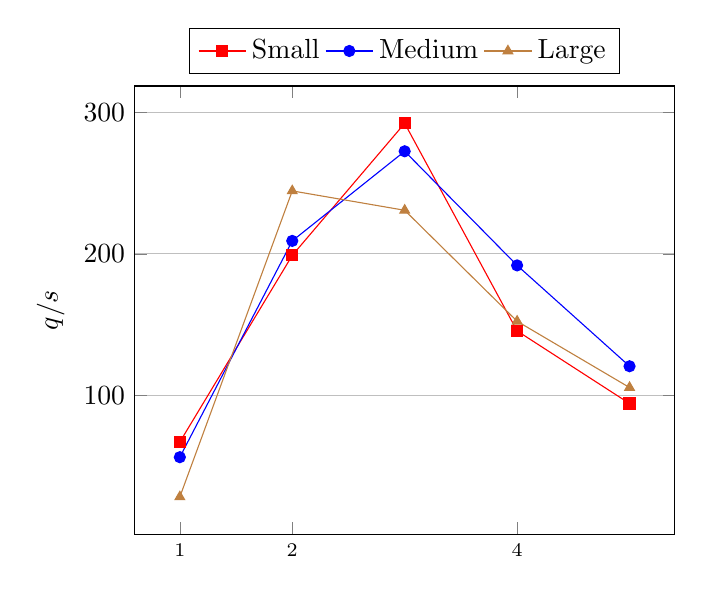
\begin{tikzpicture}
\begin{axis}[
ylabel=$q/s$,
x tick label style={font=\scriptsize},
legend style={at={(0.5,1.13)}, anchor=north, legend columns=-1},
xtick={1,2,4,8,16},
%ybar,
ymajorgrids=true,
%bar width=5pt,
]

\addplot[red,mark=square*]
coordinates {(1, 66.884) (2, 198.906) (3, 292.334) (4, 145.492) (5, 94.124)};
\addplot[blue,mark=*]
%coordinates {(1, 56.163) (2, 209.161) (3, 272.554) (4, 31.234) (5, 120.493)};
coordinates {(1, 56.163) (2, 209.161) (3, 272.554) (4, 191.828) (5, 120.493)};
\addplot[brown,mark=triangle*]
coordinates {(1, 28.062) (2, 244.529) (3, 230.814) (4, 152.311) (5, 105.441)};

\legend{Small, Medium, Large}

\end{axis}
\end{tikzpicture}%

  	}
  	\label{fig:low-query-rate}
  }\quad%
  \subfloat[Query rate with MH selectivity]{%
    \resizebox{0.45\linewidth}{!}{%
      
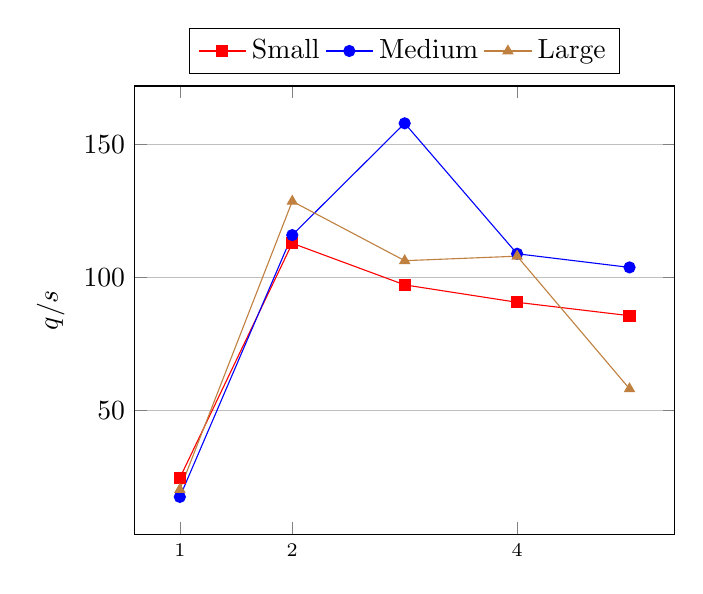
\begin{tikzpicture}
\begin{axis}[
ylabel=$q/s$,
x tick label style={font=\scriptsize},
legend style={at={(0.5,1.13)}, anchor=north, legend columns=-1},
xtick={1,2,4,8},
%ybar,
ymajorgrids=true,
%bar width=5pt,
]

\addplot[red,mark=square*]
coordinates {(1, 24.614) (2, 112.895) (3, 97.257) (4, 90.697) (5, 85.659)};
\addplot[blue,mark=*]
coordinates {(1, 17.492) (2, 115.986) (3, 158.028) (4, 108.956) (5, 103.826)};
\addplot[brown,mark=triangle*]
coordinates {(1, 20.265) (2, 128.696) (3, 106.352) (4, 108.047) (5, 58.153)};

\legend{Small, Medium, Large}

\end{axis}
\end{tikzpicture}%

    }
    \label{fig:medium-query-rate}
  }%
	\caption{The evolution of the average query rate with respect to the size of the star queries over different dataset size.}
	\label{fig:query-rate}
\end{figure}

\section{Discussion}

While AFOR provides better compression ratio than PFOR, AFOR-2 is slower than
PFOR on position file, suggesting that PFOR exception management is slightly
more efficient than the variable frame length approach of AFOR-2 on very
sparse lists. The number of table lookups in AFOR-2 costs more than the
decoding and patching of the exceptions in PFOR.

In general, FOR even if it has more data to read and decompress still provides
the best query execution time. The reason is that our experiments are
performed using warm cache. We therefore ignore the cost of disk IO
accesses and so we can expect a drop of performance for algorithms with a low
compression ratio such as FOR and PFOR compared to AFOR when executing with a
cold cache.

% Compression and decompression performance do not only depend on the
% compression ratio, but also on the execution flow of the algorithm and the
% number of cycles needed to compress or decompress an integer. Therefore,
% CPU-optimised algorithms providing good compression ratio increase the update
% and query throughputs of web search engines. In that context, AFOR seems to be
% a good candidate since it is well balanced in all aspects: it provides very
% good indexing and querying performance and one of the best compression ratio.
% 
% The Simple encoding family is somehow similar to AFOR. At each iteration, S-64
% encodes or decodes a variable number of integers using CPU optimised routines.
% AFOR is however not tied to the machine words, is simpler to implement and
% provides better compression ratio, compression speed and decompression speed.


\chapter{Self-Indexing Benchmarks}{%
In this section we will discuss the performance of SkipBlock compared to Skip
Lists by building structures on real data and performing set operations. First
we present the benchmarking environment used for comparing the self-indexing
structures. Then we compare the results of the SkipBlock structure to the
theoretical ones, before discussing the benefits of the block-based
self-indexing structure against the original Skip List. }%
\label{chap:self-indexing-bench}
\section{Benchmarking Framework}

The benchmarking framework is the same as in
Chapter~\ref{chap:benchmark-cmp}. In this section I present the benchmark
environment used to evaluate the self-indexing structures.

\subsection{Dataset}

For this benchmark we use inverted lists extracted from the Sindice dataset
from Section~\ref{sec:benchmark:framework-cmp}. Those inverted lists only
contains the entity identifiers values, the self-indexing structures being
built upon an ordered list of records, and since only the raw performance of the
self-indexing structure is measured. The other identifiers (e.g., attributes
or values identifiers) are only relevant when computing queries, thus they are
discarded for this benchmark. A small set from each frequency groups, i.e.,
HIGH, Medium and LOW groups generation presented in
Section~\ref{sec:bench-query-FW}, is extracted but keeping the entities
identifiers stream only. A list from the HIGH group will be longer than one
from the LOW group.

\subsection{Benchmark Design}

In order to have a better view of the raw performance of the self-indexing
structures, we perform two set operations, \emph{exclusion} and
\emph{conjunction}. The lists operated on are taken from one of the
three frequency groups of the Sindice dataset. Conjunction operations perform
the intersection of n lists given as operands. Exclusion operations $L_a
\backslash L_b$ exclude all the records from $L_b$ in $L_a$.

This design is based on the querying benchmark's design from the
Section~\ref{sec:bench-query-FW}. In order to process conjunctive queries, the
inverted lists from each term of the query are retrieved and intersected as
explained in Chapter~\ref{chap:IR}. To process the Boolean operator NOT,
the inverted list of the term the operator is affected to is excluded from the
results. At the core of queries processing, set operation are performed on the
retrieved lists. Based on the notation of the Section~\ref{sec:bench-query-FW},
the conjunction set operation of two inverted lists reflects the same
underlying process when computing 2-AND queries.
A measurement of the evaluation consists in the average time to execute a set
operation.

The benchmark records four information:
\begin{enumerate}
  \item the number of bytes read from the self-indexing structure.
  \item the number of documents identifiers skipped.
  \item the average time needed to perform 1 measure.
  \item the total number of search operations done on the structure as defined
  in Section~\ref{sec:cost-based-cmp}, composed of the number of
  synchronization points read plus the number of records scanned.
\end{enumerate}

The design of the SkipBlock benchmark includes two factors:
\begin{description}
\item[Operands] having two levels: HIGH-HIGH and HIGH-LOW. For instance, the
former value means that there are two operands, the HIGH and LOW inverted lists.
\item[Operation] having two levels: exclusion and conjunction.
\end{description}
Each condition of the design, i.e., HIGH-HIGH, Conjunction, possesses 100
distinct measurements.

\subsection{Implementations}

The SkipBlock model possess two implementations based on the interval search
strategies introduced in Section~\ref{sec:search-interval}. However only the S1
and S2 strategies will be discussed in these results due to a lack of time to
evaluate the others.
\begin{itemize}
  \item The baseline \emph{$I_1$} is the original Skip Lists structure with the
  linear search strategy \emph{S1}.
  \item The implementations \emph{$I_2$} and \emph{$I_3$} use respectively the
  strategies \emph{S1} and \emph{S2}. As a remainder, the S2 strategy uses
  block headers as additional synchronization points within an interval.
\end{itemize}

\section{Results}

For these benchmarks, both the self-indexing structures and the inverted list
are compressed with the VByte algorithm.
Before experimenting on the set operations, we evaluated the performance of the
self-indexing structures solely on skipping records. We first review the
evaluation results on the raw performance of the structures, before discussing
the performance with set operations.

\subsection{Advancing on a List}

In this section we evaluate the raw performance of both self-indexing models to
advance on an ordered list. The Table~\ref{tab:skipping-len} reports these
results on a list of $6\times 10^{8}$ records, records that only consist of
entity identifiers.
The first two rows reports the size in MBytes of the self-indexing structures.
A sequence of equally spaced candidates are searched,
i.e., a small skipping length of 16 and a large one of $13\times 10^{4}$
records. For each skipping length, the self-indexing structure are
parameterized with intervals of 32 and 1024, yielding for SkipBlock
respectively two possible configurations ($\vert B \vert =8, \;p=4$) and
($\vert B \vert =64, \;p=16$). 

For a same interval $\vert I \vert$ the SkipBlock structures
performs less search operations, thus saving CPU cycles as the
Table~\ref{tab:cmp-costs} have shown this aspect. However this benefit is
outweighted by the structure's size on small intervals (i.e., $\vert I \vert =
32$), since more data has to be read into memory.
Despite the predicted processing times reported in the
Table~\ref{tab:predicted-times}, the actual processing time for the SkipBlock
structure is not what was expected, i.e., half the time of the original Skip
List's. This can be explained by the compression algorithm, VByte, which is not
suited for compressing blocks.

We can note that for large skip lengths (i.e., 130 000) the SkipBlock
structures are more than 2 times as fast as the original Skip List, on large
intervals. The reason is that for so large intervals the baseline has its
number of levels considerably reduced, which is not the case for SkipBlock
since it adds in-between levels (e.g. Table~\ref{tab:skip-levels}). On top of
these additional levels, $I_3$ allow to reduce the number of search operations
by 10 times in comparison to the baseline.
When performing small skips, $I_2$ and $I_3$ implementations provide better
time than $I_1$ on large interval.

This experiment showed that the SkipBlock model provides important benefits
when jumping over a large number. With small skipping lengths, more data is
read from the SkipBlock as there are additional levels. In the latter case the
benefit of additional skipping levels is outweighted by the increased amount
of read data. We can conclude that in order to get the most benefit from
SkipBlock, configurations with large interval lengths are the most suited.

\begin{table}
\centering
\resizebox{\linewidth}{!}{%
\begin{tabular}{llc@{\hs}lllc@{\hs}lllc@{\hs}lll}
\toprule
 & $\vert I \vert$ & \phantom{a} & \multicolumn{3}{c}{$I_1$}
& \phantom{a} & \multicolumn{3}{c}{$I_2$} & \phantom{a} &
\multicolumn{3}{c}{$I_3$} \\
\cmidrule{4-6} \cmidrule{8-10} \cmidrule{12-14}
& 32 & \phantom{a} & \multicolumn{3}{c}{40.37 MB} & \phantom{a}&
\multicolumn{3}{c}{83.09 MB} & \phantom{a} & \multicolumn{3}{c}{297.57 MB} \\
& 1024 & \phantom{a} & \multicolumn{3}{c}{2.24 MB} & \phantom{a}&
\multicolumn{3}{c}{2.57 MB} & \phantom{a} & \multicolumn{3}{c}{31.6 MB} \\

\midrule
Length & & \phantom{a} & MB & Time & Ops
& \phantom{a} & MB & Time & Ops
& \phantom{a} & MB & Time & Ops \\
\multirow{2}{*}{16} & 32
&\phantom{a}& 38.11 & 12.9
s $\pm$ 135.1 ms & \numprint{338104836} 
&\phantom{a}& 59.72 & 13.8 s $\pm$ 96.8
ms & \numprint{324999973}
&\phantom{a}& 131.25 & 19.3 s $\pm$
132.1 ms & \numprint{212499973} \\
& 1024
&\phantom{a}& 2.24 & 12.6 s $\pm$ 117.7
ms & \numprint{591797454}
&\phantom{a}& 2.46 &
12.0 s $\pm$ 208.6 ms & \numprint{591250005}
&\phantom{a}& 29.28 & 14.0 s $\pm$
88.7 ms & \numprint{459999997} \\
\\
\multirow{2}{*}{\numprint{130000}} & 32
&\phantom{a}& 0.54 &
48.0 ms $\pm$ 5.8 ms & \numprint{211963}
&\phantom{a}& 0.30 & 42.3 ms $\pm$ 8.8 ms
& \numprint{109174}
&\phantom{a}& 0.31 & 47.8 ms $\pm$ 3.1 ms
& \numprint{95326} \\
& 1024
&\phantom{a}& 2.10 & 112.7 ms $\pm$
3.5 ms & \numprint{2883453}
&\phantom{a}& 0.33 & 46.1 ms $\pm$ 2.8 ms
& \numprint{2398582}
&\phantom{a}& 0.44 & 39.5 ms $\pm$ 2.1 ms
& \numprint{283796} \\
\bottomrule
\end{tabular}}
\caption{Self-indexing structures performance with equally spaced (i.e.,
$Length$) candidates. \emph{MB} stands for the number of MBytes read from the
structure. $Ops$ reports the total number of search operations performed
(i.e., the number of synchronization points read plus the number of scanned
records).}
\label{tab:skipping-len}
\end{table}

\subsection{Set Operations Results}
\label{sec:self-indexing-res}

For these benchmarks, both the self-indexing structures and the inverted list
are compressed with the VByte algorithm, so that the differences in
performance between the two structures are not caused by the compression
technique.

The performance of the self-indexing structures is compared based on the time
to perform a set operation, on the number of records that had to be scanned
from the inverted list to search for the candidates, and on the size of the
structure. We can note that the The raw results are reported in the
Table~\ref{tab:conjunction} and Table~\ref{tab:exclusion} in the appendix. For
each operands type (i.e., HIGH:HIGH or HIGH:LOW) and implementations, the best
execution time is taken and reported in the plots of the
Figure~\ref{fig:conj-excl-res}.

We observe from the plots that for either operations on two large lists (i.e.,
HIGH:HIGH type), the SkipBlock configuration of the implementation $I_3$
provides slightly better time than the original while reducing the number of
scanned records by $10^7$. However this has an impact on the structure's size
with an increase of 20 MBytes in comparison to the original model. With set
operations over lists of different sizes (i.e., LOW:HIGH type), we observe the
opposite: by scanning slightly more records and with comparable running times,
the implementation $I_3$ halves the structure's size by at least two.

For set operations on very dense lists, we are able to skip over a large number
of records with the SkipBlock model by increasing the structure's size, while
still providing similar running time as the original model. For set operations
on lists presenting a high size discrepancy, the SkipBlock model is able to
greatly reduce the structure's size while still providing similar running times.

With regards to the raw results of the Appendix~\ref{app:self-indexing:results},
this comforts the conclusion of the previous section that the SkipBlock model
provides more benefits with large intervals. We can note that the implemented
search strategies on intervals are simple ones. Thus it is possible to improve
performances by either changing the strategy, or by using an other compression
method. Indeed we used for this benchmark the VByte algorithm which is not a
block-based algorithm and thus does not profit from all the advantages of the
SkipBlock model. With a compression technique such as AFOR, we are effectively
able to reduce the size of the structure by using the frame skipping technique
(Section~\ref{sec:afor-skip}).

We can conclude that the SkipBlock model provides implementations, on large
interval lengths (e.g., 4096), that trade the structure's size cost over its
searching cost.

\begin{figure}
\centering
\resizebox{\linewidth}{!}{%
\subfloat[Two HIGH operands.] {

\begin{tikzpicture}
\begin{axis}[
        scatter/classes={
		a={mark=o},
		b={mark=star},
		c={mark=square}
% 		d={mark=diamond},
% 		e={mark=triangle}
  },
  xlabel=$Time \; (s)$,
  ylabel=$Scans$,
  mark options={scale=2},
  legend style={font=\scriptsize},
]

\addplot[red,scatter, only marks]
plot[scatter src=explicit symbolic]
coordinates {
% 	(3.400, 55766922) [a]
% 	(2.492, 55882733) [b]
% 	(2.484, 65538236) [c]
% 	(2.541, 73415418) [d]
% 	(2.619, 85376552) [e]

% 	(3.400, 50197056) [a]
% 	(2.492, 52524966) [b]
% 	(2.484, 64766407) [c]
% 	(2.541, 72983836) [d]
% 	(2.619, 85129635) [e]
	
	(2.484, 64766407) [a]
	(2.517, 72893207) [b]
	(2.582, 54730557) [c]
};

\addplot[blue,scatter, only marks]
plot[scatter src=explicit symbolic]
coordinates {
	(16.836, 54212443) [a]
	(15.826, 54205740) [b]
	(15.783, 42438570) [c]
};

% \addplot+[blue,scatter, only marks]
% plot[scatter src=explicit symbolic]
% coordinates {
% % 	(3.631, 53390244) [a]
% % 	(2.650, 54471140) [b]
% % 	(2.844, 65153966) [c]
% % 	(2.517, 73224689) [d]
% % 	(2.925, 85264977) [e]
% 	(3.631, 47270398) [a]
% 	(2.650, 51058497) [b]
% 	(2.844, 64576706) [c]
% 	(2.517, 72893207) [d]
% 	(2.925, 85080396) [e]
% };
% 
% \addplot+[green,scatter, only marks]
% plot[scatter src=explicit symbolic]
% coordinates {
% % 	(3.746, 53680730) [a]
% % 	(3.795, 53203556) [b]
% % 	(2.646, 54160474) [c]
% % 	(2.627, 56475877) [d]
% % 	(2.582, 56514322) [e]
% 	(3.746, 33665878) [a]
% 	(3.795, 42187630) [b]
% 	(2.646, 51063586) [c]
% 	(2.627, 54730109) [d]
% 	(2.582, 54730557) [e]
% };

\legend{$I_1$, $I_2$, $I_3$}
\end{axis}
\end{tikzpicture}

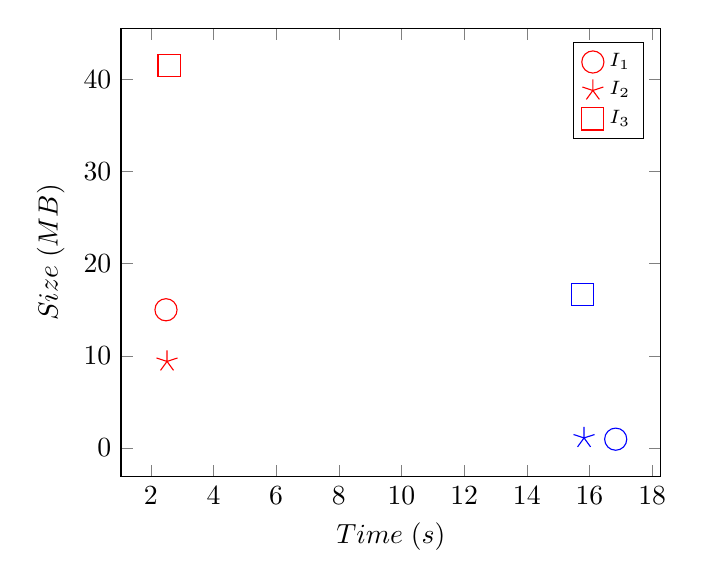
\begin{tikzpicture}
\begin{axis}[
        scatter/classes={
		a={mark=o},
		b={mark=star},
		c={mark=square}
% 		d={mark=diamond},
% 		e={mark=triangle}
  },
  xlabel=$Time \; (s)$,
  ylabel=$Size \; (MB)$,
  mark options={scale=2},
  legend style={font=\scriptsize},
  legend pos= north east
]

\addplot[red,scatter, only marks]
plot[scatter src=explicit symbolic]
coordinates {
% 	(3.400, 12.02) [a]
% 	(2.492, 7.36) [b]
% 	(2.484, 2.97) [c]
% 	(2.541, 1.66) [d]
% 	(2.619, 0.95) [e]
	
	(2.484, 15) [a]
	(2.517, 9.39) [b]
	(2.582, 41.53) [c]
};

\addplot[blue,scatter, only marks]
plot[scatter src=explicit symbolic]
coordinates {
	(16.836, 0.941) [a]
	(15.826, 1.076) [b]
	(15.783, 16.69) [c]
};

% \addplot+[blue,scatter, only marks]
% plot[scatter src=explicit symbolic]
% coordinates {
% 	(3.631, 14.10) [a]
% 	(2.650, 9.16) [b]
% 	(2.844, 2.25) [c]
% 	(2.517, 1.30) [d]
% 	(2.925, 0.74) [e]
% };
% 
% \addplot+[green,scatter, only marks]
% plot[scatter src=explicit symbolic]
% coordinates {
% 	(3.746, 40.83) [a]
% 	(3.795, 23.87) [b]
% 	(2.646, 7.60) [c]
% 	(2.627, 4.99) [d]
% 	(2.582, 4.81) [e]
% };

\legend{$I_1$, $I_2$, $I_3$}
\end{axis}
\end{tikzpicture}


}}\quad
\resizebox{\linewidth}{!}{%
\subfloat[Two operands, one HIGH and one LOW.] {

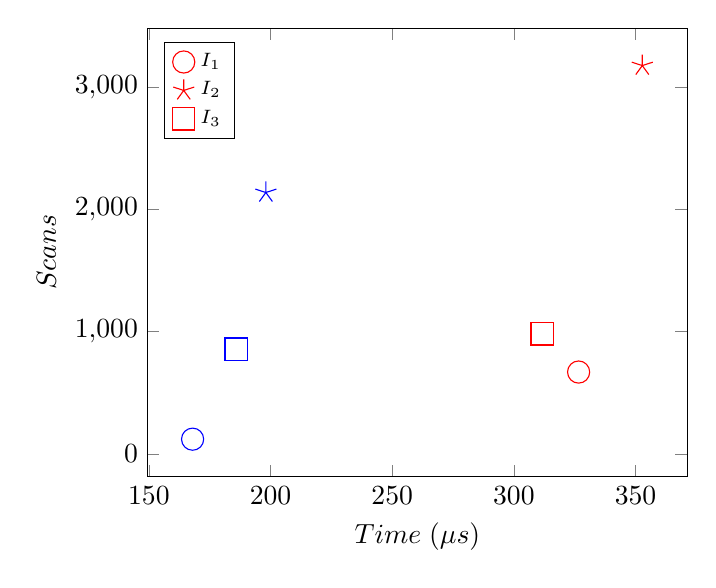
\begin{tikzpicture}
\begin{axis}[
        scatter/classes={
		a={mark=o},
		b={mark=star},
		c={mark=square}
% 		d={mark=diamond},
%  		e={mark=triangle}
  },
  xlabel=$Time \; (\mu s)$,
  ylabel=$Scans$,
  mark options={scale=2},
  legend style={font=\scriptsize},
  legend pos= north west
]

\addplot[red,scatter, only marks]
plot[scatter src=explicit symbolic]
coordinates {
% 	(363.501, 1398) [a]
% 	(326.611, 2088) [b]
% 	(545.605, 9659) [c]
% 	(579.102, 13397) [d]
% 	(735.205, 24296) [e]

% 	(363.501, 447) [a]
% 	(326.611, 670) [b]
% 	(545.605, 4315) [c]
% 	(579.102, 8407) [d]
% 	(735.205, 16207) [e]

	(326.611, 670) [a]
	(352.783, 3176) [b]
	(311.572, 982) [c]
};

\addplot[blue,scatter, only marks]
plot[scatter src=explicit symbolic]
coordinates {
	(167.969, 121) [a]
	(198.083, 2138) [b]
	(185.840, 858) [c]
};

% \addplot+[blue,scatter, only marks]
% plot[scatter src=explicit symbolic]
% coordinates {
% % 	(581.592, 932) [a]
% % 	(521.191, 990) [b]
% % 	(352.783, 3176) [c]
% % 	(432.813, 5718) [d]
% % 	(453.247, 8605) [e]
% 	(581.592, 329) [a]
% 	(521.191, 489) [b]
% 	(352.783, 2733) [c]
% 	(432.813, 5292) [d]
% 	(453.247, 8100) [e]
% };
% 
% \addplot+[green,scatter, only marks]
% plot[scatter src=explicit symbolic]
% coordinates {
% % 	(640.820, 862) [a]
% % 	(585.107, 820) [b]
% % 	(381.714, 1102) [c]
% % 	(370.581, 1539) [d]
% % 	(311.572, 1739) [e]
% 	(640.820, 150) [a]
% 	(585.107, 234) [b]
% 	(381.714, 521) [c]
% 	(370.581, 982) [d]
% 	(311.572, 982) [e]
% };

% \legend{16, 32, 256, 512, 1024}
\legend{$I_1$, $I_2$, $I_3$}
\end{axis}
\end{tikzpicture}

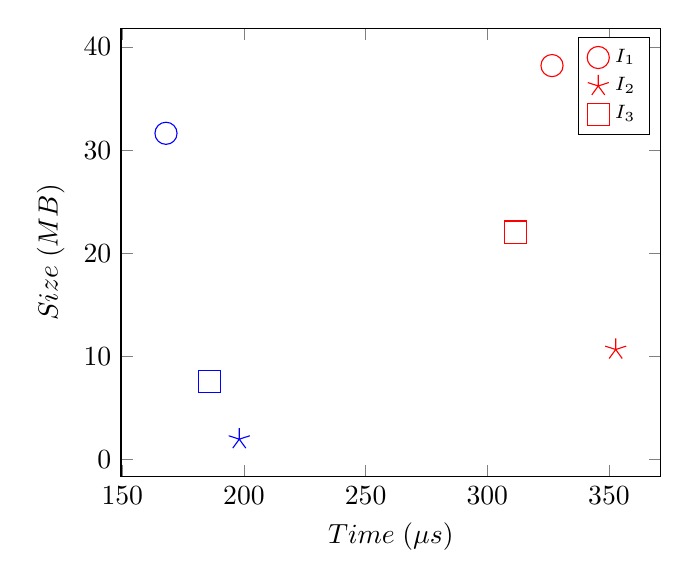
\begin{tikzpicture}
\begin{axis}[
        scatter/classes={
		a={mark=o},
		b={mark=star},
		c={mark=square}
% 		d={mark=diamond},
%  		e={mark=triangle}
  },
  xlabel=$Time \; (\mu s)$,
  ylabel=$Size \; (MB)$,
  mark options={scale=2},
  legend style={font=\scriptsize},
%   legend pos= north west
]

\addplot[red,scatter, only marks]
plot[scatter src=explicit symbolic]
coordinates {
% 	(363.501, 0.004) [a]
% 	(326.611, 0.006) [b]
% 	(545.605, 0.024) [c]
% 	(579.102, 0.022) [d]
% 	(735.205, 0.032) [e]
	
	(326.611, 38.2) [a]
	(352.783, 10.65) [b]
	(311.572, 22.05) [c]
};

\addplot[blue,scatter, only marks]
plot[scatter src=explicit symbolic]
coordinates {	
	(167.969, 31.63) [a]
	(198.083, 1.95) [b]
	(185.840, 7.57) [c]
};

% \addplot+[blue,scatter, only marks]
% plot[scatter src=explicit symbolic]
% coordinates {
% 	(581.592, 0.0031) [a]
% 	(521.191, 0.0026) [b]
% 	(352.783, 0.0023) [c]
% 	(432.813, 0.0023) [d]
% 	(453.247, 0.0027) [e]
% };
% 
% \addplot+[green,scatter, only marks]
% plot[scatter src=explicit symbolic]
% coordinates {
% 	(640.820, 0.0034) [a]
% 	(585.107, 0.0028) [b]
% 	(381.714, 0.0027) [c]
% 	(370.581, 0.0027) [d]
% 	(311.572, 0.0034) [e]
% };

\legend{$I_1$, $I_2$, $I_3$}
\end{axis}
\end{tikzpicture}
}}
\caption{Conjunction (in red) and exclusion (in blue) set operations. The time
on the x axis is the best average time, from the
Appendix~\ref{app:self-indexing:results}, to perform the operation on the
given operands for an implementation.}
\label{fig:conj-excl-res}
\end{figure}


\part{Additional Work and  Conclusion}
\label{part:conclusion}
\chapter{SIREn Query Parser}{
The query parser is used in SIREn in order to allow people to interact with its
index. However we must keep in mind that Sindice, which uses SIREn for
searching and browsing purpose, is aimed to be used as a web service by machine
as well. In this section, we present a query parser that matches triple
patterns in datasets before describing a parser that matches entities.
}
\label{chap:siren-extension}
\section{NTriple Query Parser}
\label{sec:N3-qparser}

As with the SPARQL language, the NTriple query parser aims to find sub-graph
within datasets that best match a given set of triple patterns. Triple patterns
are linked together thanks to Boolean operators, i.e. AND, OR, NOT. To express
such patterns, SIREn uses a bottom-up grammar, and is built as a plugin to the
Lucene\footnote{Lucene: \url{http://lucene.apache.org/}} query parser.
\begin{description}
  \item[Literals] any string enclosed between simple quotes are taken as a
  literal.
  \item[Literal Pattern] any string enclosed between double quotes. It
  describes the pattern that has to appear within the object of the returned
  triples for the query, thanks to Boolean operations.
  \item[URIs] any string enclosed between the characters '$<$' \whs '$>$'.
\end{description}
Any part of a triple pattern, to a maximum of two per triple, can be left
unknown thanks to the wildcard character '*'. Any term of the query can be
flagged in order to indicate if the term has to, must not or may appear within
the triples in the results by using respectively the characters '+', '-', ''
(i.e no character). Considering URIs are tokenism when indexing (e.g.
\url{http://sindice.com/} is tokenism into ``HTTP'', ``Sindice'' and ``com''),
the following query
\begin{quotation}
$<$rings$>$ $<$author$>$ ``j.r.r.\_tolkien OR tolkien'' .
\end{quotation}
matches the RDF graph of the Figure~\ref{fig:rdf-graph}. The object of this
triple pattern is a literal pattern, which aims to widen the search to several
writings of the author's name. Since SIREn is an Information Retrieval search
engine, it processes the query as explained in Chapter~\ref{sec:IR} with set
theory operations (i.e. conjunction, disjunction and exclusion).

During indexing, it is possible to store into a specific field any text. For
instance, one can have three different fields such as ``title'', ``author'' and
``abstract'' for the entities in the Figure~\ref{fig:entities}. This way the
abstract of the entity \emph{\_:bnode1} would fall into its field, allowing for
more precise search. A field is identified with the special Lucene character
semi-colon, ':'. For instance the term ``hobbit'' within the entity \_:bnode1
can be refer ed as \emph{abstract{\bfseries :}hobbit}. 

\subsection{Added Features}

The SIREn query parser has been extended to support commonly used feature in
RDF and also to be more expressive. In this section three added features are
presented.

\paragraph{URI Pattern}

As with literal patterns, this extension allows to use Boolean operators within
an URI. It is then possible for example to search for RDF graphs where some
URI(s) contains both the terms \emph{lord} and \emph{rings} by entering the
query \emph{$<$lord AND rings$>$ * * .}$\;$.

\paragraph{Qualified Name - QName}

As explained in the introduction to Information Retrieval in
Chapter~\ref{sec:IR}, a QName is a term that is used to abbreviate an URI.
Whiting an URI, it is possible to use a QName by appending the term to the
semi-colon character. The QName is replaced at query processing time by the
correct namespace thanks to a file containing the mapping between a QName and
its expansion.
This expansion is performed on any string that matches a QName format only
within an URI, and in that case leaves the term unchanged if no mapping key has
been found. Restricting the substitution to URIs allows to QNames-like strings
within literals.

A QName can possess several expansion, e.g. the web
site\footnote{QNames namespace lookup for developers:
\url{http://prefix.cc/}} reports that the QName \emph{dbpedia} is mapped to
three possible expansion
\begin{enumerate}
  \item \url{http://dbpedia.org/resource/}
  \item \url{http://dbpedia.org/dbprop/}
  \item \url{http://dbpedia.org/property/}
\end{enumerate}
In order to deal with multi-valued QNames, all possible expansion replace their
QName, linked together with the Boolean operation OR. For instance the query
\begin{quotation}
* $<$\textcolor{red}{dbpedia}:\textcolor{blue}{title}$>$ * .
\end{quotation}
is expanded to
\begin{quotation}
\resizebox{\linewidth}{!}{%
* $<$\textcolor{red}{\url{http://dbpedia.org/resource/}}
\textcolor{blue}{title} OR
\textcolor{red}{\url{http://dbpedia.org/dbprop/}}\textcolor{blue}{title} OR
\textcolor{red}{\url{http://dbpedia.org/property/}}\textcolor{blue}{title}$>$ * .
}%
\end{quotation}
This expansion is rendered possible thanks to the URI pattern extension of an
URI presented previously. Thus it allows to perform more generic search and to
abstract from the actual schema definition the RDF graphs possess.

\paragraph{Multi-field search}

SIREn is based on Lucene, which data representation model uses fields. Fields
allows to organize logically the information. For example we can split the
documents from the collection according to their dataset, so that all documents
from a same dataset are within the same field.

However spitting information into fields implies that we lose a global view of
the data. To cope with this drawback, we have implemented an extension to the
query parser that search documents across fields, enabling the retrieval of
triple patterns regardless of the field it actually occurs. Moreover depending
on the reliability or the importance that is given to field, it is possible to
affect a \emph{weight} value to that field.

As an example, below is shown a RDF graph with two triples taken from two
different datasets: ``dataset1'' and ``dataset2''
\begin{quotation}
dataset1: $<$http://s$>$ $<$http://p1$>$ ``literal'' .

dataset2: $<$http://s$>$ $<$http://p2$>$ $<$http://o2$>$ .
\end{quotation}
While the query with two triple patterns
\begin{quotation}
($<$http://s$>$ * 'literal' .) AND ($<$http://s$>$ *
$<$\textcolor{blue}{http://o2}$>$ .)
\end{quotation}
matches the previous graph thanks to the implicit link, i.e., the first pattern
returns the triple from dataset1 and the second one from dataset2, the query
\begin{quotation}
($<$http://s$>$ * 'literal' .) AND ($<$http://s$>$ *
$<$\textcolor{blue}{http://o1}$>$ .)
\end{quotation}
does not, since the second pattern cannot be found.

\section{Entity Query Parser}
\label{sec:ent-qparser}

With the semantic web representation model such as RDF, we can describe people,
products, countries or any other entities. When searching for information we
often want results that are relevant for a specific entity, any other results
polluting the information retrieved. As a first step, SIREn is indexing
entities with an entity-centric rather than a document-centric model. The
second step is to build a parser that handles queries for an entity.

The entity query parser is being developed which goal is to matcher patterns for
an entity. For example we will able to formulate the query ``Find all the
people within DERI that are from France''. To better represent relations
between an entity and other entities or objects, we use a one-to-many
representation model called the \emph{tabular} format. The
Table~\ref{tab:tabular-format} depicts triples in a document-centric
representation on the left, and its tabular view on the right. With the tabular
format we define as a field the predicate (i.e., attribute) and store within
that field all the related objects. To answer the previous example query, we
can have two fields in the entity description of DERI, the countries and the
people fields.

For such queries to be efficient the schema of the data has to be known. As
such this parser is intended to be use over specific datasets, such as the
intranet of a company.

\begin{table}
\ra{0.3}
\centering
\begin{tabular}{lllc@{\hs}ll}
\toprule
\multicolumn{3}{c}{Document-centric} & \phantom{a} & \multicolumn{2}{c}{Tabular
format} \\
$<$ s $>$ & $<$ p1 $>$ & $<$ o1 $>\;.$ & \phantom{a} &
\multirow{2}{*}{$<$ o1 $> \; <$ o2 \; o3 $>$} \\
$<$ s $>$ & $<$ p2 $>$ & $<$ o2 $> \; <$ o3 $>\;.$ & \phantom{a} & & \\
\bottomrule
\end{tabular}
\caption{The tabular format data representation.}
\label{tab:tabular-format}
\end{table}


\chapter{Conclusion}{
In the recent years, the amount of semantic data has considerable increased.
More and more web sites are exporting their data using RDF, as the power of the
semantic web is increasingly attractive: to be able to efficiently search
across multiple data sources specific information, and to retrieve relevant
results hereafter. The semantic Web is a challenging and expanding research
domain. The Web as we know it is undergoing a radical change, and the semantic
web is contributing a lot to it.

People are publishing RDF data following the best practices of Linked Data. The
Linking Open Data Cloud is a huge gathering of inter-connected semantic data
sources. Applications can use this linked data and provide a concrete benefit
to the way we use the Web. \emph{Sig.ma} is a use case for a mashup application
that shows the power of the semantic. Its purpose is to search across many
data sources, and to provide information organized around \emph{entities},
e.g., a product, a person or any other concept. To be able to efficiently use
this collection of knowledge of we scale so that applications like Sig.ma are
viable is an important and challenging matter. Sig.ma is built on
\emph{Sindice}, a web service that provides search and retrieval capabilities
over semantic data. The web service uses \emph{SIREn} at its core, an
Information Retrieval search engine, to query an \emph{information need} and
to retrieve \emph{relevant} documents.

In this report we presented data structures that are commonly used in
Information Retrieval search engines. We also discussed about some of the
focusing points for optimizing these structures in order to have more efficient
and scalable IR search engines like SIREn.
We presented AFOR, a compression method that provides both fast compression
(increases index updates) and decompression (increases query throughput) speed,
and yet with a high compression ratio. We proposed SkipBlock, a novel
self-indexing model where some configurations carefully chosen provide faster
random lookups from an inverted list and a more compact structure than the
original Skip List model.}
\label{chap:conclusion}

\section{Summary of the Report}

The flow of this report reflects the flow of a research work by
\begin{inparaenum}[(1)]
\item describing a problem and why current related work do not answer the
requirements;
\item proposing a solution to the problem; and
\item proving the previous claims by performing comparative benchmarks.
\end{inparaenum}
Following this pattern, we proposed two novel structures, where both have the
common goal to reduce the amount of data read in order to increase the IO
throughput. 
\begin{description}
\item[Compression Technique] compression techniques do not only aim at reducing
the storage space, but also at increasing the IO access time. Reading/writing
less data from/to disk with a high performance algorithm reduce the wasted time
on IO access. Thus the performance of operations that directly depends on some
data to process is improved. We proposed \emph{AFOR}, a new compression class
that can increase query throughput compared to other state of the art
algorithms thanks to a more ``close-to-data'' compression.
\item[Self-Indexing Technique] query processing returns relevant information by
applying some operations on the inverted lists. However not all the data that
inverted lists have is necessary, thus reading or decoding such data is a
wasted time. Self-indexing is a technique that allows to skip over portions of
the inverted lists that are unnecessary for the processing of a query. We
proposed a new self-indexing model, called \emph{SkipBlock}, that aims to
improve the original model Skip List by taking into consideration the
compression algorithm used on the inverted lists. We will also present at
\emph{The $33^{rd}$ European Conference on Information Retrieval}
(ECIR)\footnote{ECIR: \url{http://www.ecir2011.dcu.ie/}} the paper which
introduced the model (Appendix~\ref{app:SkipBlock-paper}).
\end{description}

\section{Future Work}

The Information Retrieval domain for Semantic Data covers not only what has
been presented in this report but a wider area of problems. In the coming
months, I will stay within DERI and work on different subjects. In this section
I list a number of the possible future work.
\begin{itemize}
  \item Finalize the AFOR implementation to make it into a production ready
  state.
  \item Continue the research on SkipBlock, which will consists in optimizing
  search strategies and finding more adapted ones.
  \item Implement a novel SIREn index structure that will improve query
  processing performance.
  \item Start researching on dynamic query processing.
\end{itemize}

\section{Personal Benefits}

My internship at DERI has been a source for new knowledge in many areas. I was
able to deepen not only my skills in computer programming but also my
scientific knowledge.
\begin{description}
\item[Computer Skills] Thanks to this internship I was able to improve my
skills on different programming languages: in JAVA since our project SIREn
uses it, in script shell such as bash or Ruby when writing benchmarks automating
scripts, in a text stream editor like \emph{Sed}, very convenient for automate
operations on large files such as logging or benchmarking results files.
\\*[\parskip]
Because SIREn is a system built to be highly efficient and scalable over
millions of entities descriptions, any code that will be used within has to be
well written. The engineer must take care of the memory and the CPU consumption
so that the best performance is reached. Concerning JAVA there are many classes
available to help the developer, for instance it is better to use the class
\texttt{StringBuilder}\footnote{\texttt{StringBuilder}:
\url{http://tinyurl.com/3xbkvw6}} when operating of very large strings than to
use the \texttt{String} type.
\\*[\parskip]
At last it is important to comment the code written, not only for people using
it later on but also for ourselves since it permits to know its structure or
what are the possible optimizations. As part of commenting the code, writing
meaningful descriptions in SVN logs helps to keep track of what was done and
the reason of some changes.
\item[Engineering Skills] For the last months of my internship I was given a
project (the SkipBlock model) to work on alone. This experience showed me the
different points to take care of when managing projects, such as coordinating
the development with some deadline. Also when implementing a solution, there
are sometimes a difference between the model and the real results of the
implementations. This leads to the necessity of taking decisions in order to
understand why it is so and to be able to explain clearly the reasons. Moreover
it is frequent when implementing under a deadline pressure that the code isn't
optimized. In a short term this is not a problem, but in a long term it becomes
one as a \emph{technical debt}\footnote{Technical Debt:
\url{http://www.martinfowler.com/bliki/TechnicalDebt.html}}, since a messy code
will end up in re-factoring.
\item[Research Skills] DERI made me aware of the challenges that we can expect
from the research environment, such as a research dependent implementations
which change a project flow, since time constraints cannot be put on tasks
because the expecting difficulty and problems are still unknown. Moreover
working on the SIREn project allowed me to take part into the publication
process of scientific papers. These points as well as the scientific domain of
DERI (Semantic Web) and of the project (IR plus highly efficient structures)
gave me the desire to keep on working in the DI2 team for the following year.
\item[Scientific Knowledge] Thanks to this internship I was able to gain more
knowledge on the interesting Information Retrieval domain. Moreover the
internship made me aware of the Semantic Web infrastructure and of all the
possibilities it provides.
\item[Human Skills] A project cannot be successful unless the communication
between members is clear and efficient. A good communication flow allows
members to know the big picture of the research, and what should be working on
each individuals. DERI is a multi-cultural research institute, with
people form all around the world. This working environment was a good basis for
improving my English.
\end{description}

%%%%%%%%%%%%%%%%%%%%%%%%%%%%%%%%%%%%%%%%%
\appendix
% \begin{appendices}
\chapter{Benchmarking Results}

\section{Results of the Compression Benchmark}
\label{app:compression:results}

This appendix provides tables containing the results of the benchmarks that
have been performed for comparing the indexing and querying performance of the
index structure with various compression algorithms.
Tables~\ref{tab:indexing-performance} have been used for generating the charts
from Section~\ref{sec:compression:indexing-performance}.
Tables~\ref{tab:query-time} have been used for generating the charts from
Section~\ref{sec:compression:query-performance}.

\begin{table*}[h!]
	\centering
	\ra{1.3}
	\resizebox{0.8\linewidth}{!}{%
	\subfloat[Wikipedia]{%
	\begin{tabular}{@{}rcr@{\hs}rcr@{\hs}r@{\hs}r@{\hs}r@{\hs}}
	\toprule
	& \phantom{a} 
	& \multicolumn{2}{c}{Time (s)} 
	& \phantom{a} 
	& \multicolumn{4}{c}{Sizes (GB)} \\ 
	\cmidrule{3-4} \cmidrule{6-9}
	Method && Total & Opt && Doc & Frq & Pos & Total \\
	\midrule
	AFOR-1 && 410 & 114&& 0.353 & 0.109 & 0.698 & 1.160\\
	AFOR-2 && 409 & 128&& 0.340 & 0.093 & 0.655 & 1.088 \\
	FOR && 443 & 128&& 0.426 & 0.178 & 0.811 & 1.415\\
	PFOR && 438 & 127 && 0.428 & 0.106 & 0.745 & 1.279\\
	Rice && 492 & 228 && 0.332 & 0.061 & 0.600 & 0.993\\
	S9-64 && 462 & 124&& 0.356 & 0.103 & 0.662 & 1.121\\ 
	VByte && 433 & 132 && 0.402 & 0.291 & 0.714 & 1.407\\      
	\bottomrule
	\end{tabular}
	}\quad%
	\subfloat[Blog]{%
	\begin{tabular}{@{}rcr@{\hs}rcr@{\hs}r@{\hs}r@{\hs}r@{\hs}}
	\toprule
	& \phantom{a} 
	& \multicolumn{2}{c}{Time (s)} 
	& \phantom{a} 
	& \multicolumn{4}{c}{Sizes (GB)} \\ 
	\cmidrule{3-4} \cmidrule{6-9}
	Method && Total & Opt && Doc & Frq & Pos & Total \\
	\midrule
	AFOR-1 && 12337 & 4813&& 7.868 & 2.366 & 21.058 & 31.292 \\
	AFOR-2 && 13040 & 4571&& 7.387 & 2.016 & 19.492 & 28.895 \\
	FOR && 12741 & 5888&& 9.115 & 3.882 & 26.780 & 39.777 \\
	PFOR && 13972 & 5387&& 9.097 & 2.464 & 23.975 & 35.536 \\
	Rice && 14099 & 7127&& 7.145 & 1.546 & 18.160 & 26.851 \\
	S9-64 && 13152 & 5414 && 7.892 & 2.197 & 19.711 & 29.800 \\
	VByte && 12320 & 5092 && 8.630 & 5.610 & 22.063 & 36.303 \\
	\bottomrule
	\end{tabular}
	}}\quad%
	
	\subfloat[DBpedia]{%
	\resizebox{.3\linewidth}{!}{%
	\begin{tabular}{@{}rcr@{\hs}rcr@{\hs}r@{\hs}r@{\hs}r@{\hs}r@{\hs}r@{}}
	\toprule
	& \phantom{a} 
	& \multicolumn{2}{c}{Time (s)} 
	& \phantom{a} 
	& \multicolumn{6}{c}{Sizes (GB)} \\ 
	\cmidrule{3-4} \cmidrule{6-11}
	Method && Total & Opt && Ent & Frq & Att & Val & Pos & Total \\
	\midrule
	AFOR-1 && 536 & 139 && 0.246 & 0.043 & 0.141 & 0.065 & 0.180 & 0.816 \\
	AFOR-2 && 540 & 142 && 0.229 & 0.039 & 0.132 & 0.059 & 0.167 & 0.758 \\
	AFOR-3 && 562 & 158 && 0.229 & 0.031 & 0.131 & 0.054 & 0.159 & 0.736 \\
	FOR && 594 & 158 && 0.315 & 0.061 & 0.170 & 0.117 & 0.216 & 1.049 \\
	PFOR && 583 & 167 && 0.317 & 0.044 & 0.155 & 0.070 & 0.205 & 0.946 \\
	Rice && 612 & 239 && 0.240 & 0.029 & 0.115 & 0.057 & 0.152 & 0.708 \\
	S-64 && 558 & 162 && 0.249 & 0.041 & 0.133 & 0.062 & 0.171 & 0.791 \\
	VByte && 577 & 164 && 0.264 & 0.162 & 0.222 & 0.222 & 0.245 & 1.335 \\
	\bottomrule
	\end{tabular}
	}}\quad%
	\subfloat[Geonames]{%
	\resizebox{.3\linewidth}{!}{%
	\begin{tabular}{@{}rcr@{\hs}rcr@{\hs}r@{\hs}r@{\hs}r@{\hs}r@{\hs}r@{}}
	\toprule
	& \phantom{a} 
	& \multicolumn{2}{c}{Time (s)} 
	& \phantom{a} 
	& \multicolumn{6}{c}{Sizes (GB)} \\ 
	\cmidrule{3-4} \cmidrule{6-11}
	Method && Total & Opt && Ent & Frq & Att & Val & Pos & Total \\
	\midrule
	AFOR-1 && 729 & 114 && 0.129 & 0.023 & 0.058 & 0.025 & 0.025 & 0.318 \\
	AFOR-2 && 732 & 107 && 0.123 & 0.023 & 0.057 & 0.024 & 0.024 & 0.307 \\
	AFOR-3 && 724 & 103 && 0.114 & 0.006 & 0.056 & 0.016 & 0.008 & 0.256 \\
	FOR && 748 & 102 && 0.150 & 0.021 & 0.065 & 0.025 & 0.023 & 0.349 \\
	PFOR && 741 & 134 && 0.154 & 0.019 & 0.057 & 0.022 & 0.023 & 0.332 \\
	Rice && 787 & 183 && 0.133 & 0.019 & 0.063 & 0.029 & 0.021 & 0.327 \\
	S-64 && 740 & 123 && 0.147 & 0.021 & 0.058 & 0.023 & 0.023 & 0.329 \\
	VByte && 737 & 141 && 0.216 & 0.142 & 0.143 & 0.143 & 0.143 & 0.929 \\
	\bottomrule
	\end{tabular}
	}}\quad%
	\subfloat[Sindice]{%
	\resizebox{.3\linewidth}{!}{%
	\begin{tabular}{@{}rcr@{\hs}rcr@{\hs}r@{\hs}r@{\hs}r@{\hs}r@{\hs}r@{}}
	\toprule
	& \phantom{a} 
	& \multicolumn{2}{c}{Time (s)} 
	& \phantom{a} 
	& \multicolumn{6}{c}{Sizes (GB)} \\ 
	\cmidrule{3-4} \cmidrule{6-11}
	Method && Total & Opt && Ent & Frq & Att & Val & Pos & Total \\
	\midrule
	AFOR-1 && 13734 & 1816 && 2.578 & 0.395 & 0.942 & 0.665 & 1.014 & 6.537 \\
	AFOR-2 && 13975 & 1900 && 2.361 & 0.380 & 0.908 & 0.619 & 0.906 & 6.082 \\
	AFOR-3 && 13847 & 1656 && 2.297 & 0.176 & 0.876 & 0.530 & 0.722 & 5.475 \\
	FOR && 14978 & 1749 && 3.506 & 0.506 & 1.121 & 0.916 & 1.440 & 8.611 \\
	PFOR && 14839 & 2396 && 3.221 & 0.374 & 1.153 & 0.795 & 1.227 & 7.924 \\
	Rice && 15571 & 3281 && 2.721 & 0.314 & 0.958 & 0.714 & 0.941 & 6.605 \\
	S-64 && 14107 & 2163 && 2.581 & 0.370 & 0.917 & 0.621 & 0.908 & 6.313 \\
	VByte && 13223 & 3018 && 3.287 & 2.106 & 2.411 & 2.430 & 2.488 & 15.132 \\
	\bottomrule
	\end{tabular}
	}}
	\caption{Total indexing time, optimise time and index size.}
	\label{tab:indexing-performance}
\end{table*}


\begin{table*}
\centering
\ra{1.3}

	\subfloat[Value Query]{%
	\resizebox{0.48\linewidth}{!}{%
	\begin{tabular}{@{}rcr@{\hs}r@{\hs}rcr@{\hs}r@{\hs}rcr@{\hs}r@{\hs}rcr@{\hs}r@{\hs}rcr@{\hs}r@{\hs}rcr@{\hs}r@{\hs}r@{}}\toprule
	& \phantom{a}
	& \multicolumn{3}{c}{2 - AND} & \phantom{a}
	& \multicolumn{3}{c}{2 - OR} & \phantom{a}
	& \multicolumn{3}{c}{4 - AND} & \phantom{a}
	& \multicolumn{3}{c}{4 - OR} & \phantom{a}
	& \multicolumn{3}{c}{2 - Phrase} & \phantom{a}
	& \multicolumn{3}{c}{3 - Phrase} \\
	\cmidrule{3-5} \cmidrule{7-9} \cmidrule{11-13} \cmidrule{15-17} \cmidrule{19-21} \cmidrule{23-25}
	Method && $\mu$ & $\sigma$ & MB && $\mu$ & $\sigma$ & MB && $\mu$ & $\sigma$ & MB && $\mu$ & $\sigma$ & MB && $\mu$ & $\sigma$ & MB && $\mu$ & $\sigma$ & MB \\
	\midrule
	\multicolumn{1}{l}{\textbf{DBpedia}\phantom{abc}} \\
	AFOR-1
	&& 32.6 & 1.3 & 1.8
	&& 42.9 & 1.2 & 2.0
	&& 63.2 & 2.4 & 3.6
	&& 88.4 & 2.5 & 4.0
	&& 218.4 & 13.7 & 14.2
	&& 508.3 & 4.4 & 36.6 \\
	AFOR-2
	&& 37.7 & 1.2 & 1.7
	&& 47.8 & 1.7 & 1.9
	&& 74.1 & 3.0 & 3.3
	&& 98.6 & 2.5 & 3.7
	&& 253.2 & 12.9 & 13.2
	&& 569.3 & 4.6 & 33.8 \\
	AFOR-3
	&& 44.2 & 1.2 & 1.7
	&& 52.3 & 11.2 & 1.8
	&& 86.0 & 3.7 & 3.3
	&& 110.1 & 5.0 & 3.6
	&& 256.7 & 13.9 & 13.1
	&& 593.9 & 32.2 & 33.6 \\
	FOR
	&& 31.5 & 1.4 & 2.3
	&& 46.8 & 10.6 & 2.5
	&& 61.9 & 2.9 & 4.5
	&& 86.3 & 2.5 & 5.1
	&& 220.5 & 13.2 & 18.9
	&& 531.1 & 35.3 & 48.5 \\
	PFOR
	&& 44.2 & 17.1 & 2.3
	&& 52.2 & 1.3 & 2.5
	&& 83.1 & 2.7 & 4.5
	&& 106.8 & 2.6 & 5.0
	&& 225.1 & 2.7 & 16.5
	&& 521.1 & 4.5 & 41.9 \\
	Rice
	&& 75.4 & 1.6 & 1.7
	&& 98.8 & 8.9 & 1.8
	&& 148.0 & 3.1 & 3.3
	&& 190.5 & 3.7 & 3.7
	&& 604.8 & 4.9 & 12.1
	&& 1573.0 & 6.4 & 29.9 \\
% 	RiceFOR
% 	&& 63.3 & 2.6 & 
% 	&& 93.3 & 2.2 &
% 	&& 271.6 & 3.7 &
% 	&& 490.4 & &
% 	&& & &
% 	&& & & \\
	S-64
	&& 42.4 & 3.0 & 1.9
	&& 57.8 & 1.6 & 2.0
	&& 83.3 & 2.4 & 3.6
	&& 117.8 & 2.4 & 4.0
	&& 291.0 & 15.3 & 13.7
	&& 668.8 & 6.0 & 35.0 \\
	VByte
	&& 45.8 & 17.8 & 2.7
	&& 57.2 & 1.5 & 2.9
	&& 81.0 & 2.9 & 5.2
	&& 116.7 & 2.3 & 5.9
	&& 330.5 & 13.0 & 21.9
	&& 723.9 & 5.8 & 57.8 \\
	\multicolumn{1}{l}{\textbf{Geonames}\phantom{abc}} \\
	AFOR-1
	&& 29.3 & 1.5 & 1.4
	&& 30.7 & 9.2 & 1.4
	&& 62.7 & 8.8 & 2.9
	&& 59.0 & 2.8 & 2.9
	&& 35.3 & 1.8 & 1.7
	&& 60.6 & 2.0 & 3.1 \\
	AFOR-2
	&& 36.6 & 4.3 & 1.4
	&& 33.7 & 1.6 & 1.4
	&& 69.3 & 8.5 & 2.9
	&& 72.0 & 8.6 & 2.9
	&& 40.4 & 2.4 & 1.6
	&& 68.1 & 2.5 & 2.8 \\
	AFOR-3
	&& 32.6 & 1.7 & 1.3
	&& 32.8 & 1.4 & 1.3
	&& 65.5 & 3.2 & 2.7
	&& 66.0 & 2.7 & 2.7
	&& 40.1 & 1.8 & 1.5
	&& 79.5 & 2.5 & 2.7 \\
	FOR
	&& 30.4 & 8.3 & 1.5
	&& 31.7 & 1.5 & 1.5
	&& 63.4 & 4.6 & 3.0
	&& 63.4 & 2.9 & 3.0
	&& 35.8 & 12.4 & 2.2
	&& 58.9 & 4.5 & 4.1 \\
	PFOR
	&& 37.8 & 2.1 & 1.5
	&& 38.1 & 1.9 & 1.5
	&& 78.2 & 9.8 & 3.0
	&& 77.1 & 4.7 & 3.0
	&& 45.7 & 14.1 & 2.2
	&& 87.6 & 10.5 & 4.0 \\
	Rice
	&& 69.0 & 2.1 & 1.5
	&& 69.4 & 2.9 & 1.5
	&& 141.0 & 6.5 & 3.0
	&& 139.0 & 3.9 & 3.0
	&& 89.4 & 11.9 & 1.8
	&& 134.3 & 2.9 & 3.2 \\
	S-64
	&& 41.0 & 2.3 & 1.8
	&& 42.5 & 8.0 & 1.8
	&& 82.8 & 3.8 & 3.6
	&& 80.7 & 2.8 & 3.6
	&& 53.9 & 2.2 & 1.8
	&& 75.7 & 2.8 & 3.1 \\
	VByte
	&& 40.2 & 1.4 & 2.9
	&& 39.8 & 1.3 & 2.9
	&& 85.7 & 8.0 & 5.8
	&& 80.7 & 2.1 & 5.8
	&& 46.7 & 1.3 & 3.2
	&& 77.8 & 1.9 & 5.7 \\
	\multicolumn{1}{l}{\textbf{Sindice}\phantom{abc}} \\
	AFOR-1
	&& 31.4 & 1.3 & 1.8
	&& 40.6 & 1.1 & 1.9
	&& 76.7 & 2.0 & 3.5
	&& 83.6 & 19.9 & 3.7
	&& 300.3 & 2.9 & 19.1
	&& 1377.0 & 5.7 & 78.8 \\
	AFOR-2
	&& 36.8 & 1.4 & 1.6
	&& 51.9 & 14.6 & 1.7
	&& 73.5 & 2.3 & 3.2
	&& 99.3 & 13.3 & 3.4
	&& 329.9 & 3.2 & 17.5
	&& 1394.0 & 5.9 & 72.4 \\
	AFOR-3
	&& 36.3 & 1.3 & 1.6
	&& 45.6 & 1.2 & 1.7
	&& 72.0 & 3.0 & 3.1
	&& 85.6 & 2.3 & 3.2
	&& 325.0 & 4.1 & 16.9
	&& 1377.0 & 6.1 & 70.4 \\
	FOR
	&& 35.9 & 17.9 & 2.3
	&& 37.3 & 1.1 & 2.4
	&& 60.1 & 2.3 & 4.5
	&& 70.5 & 2.0 & 4.7
	&& 323.6 & 30.3 & 28.3
	&& 1382.0 & 7.8 & 116.3 \\
	PFOR
	&& 40.5 & 1.7 & 2.3
	&& 49.8 & 2.1 & 2.4
	&& 81.4 & 10.0 & 4.5
	&& 94.1 & 2.4 & 4.7
	&& 316.6 & 3.1 & 25.5
	&& 1282.0 & 6.4 & 103.0 \\
	Rice
	&& 68.5 & 2.0 & 1.8
	&& 82.4 & 1.5 & 1.9
	&& 151.0 & 3.7 & 3.6
	&& 155.8 & 2.9 & 3.7
	&& 848.3 & 14.9 & 18.6
	&& 3348.0 & 6.7 & 74.0 \\
	S-64
	&& 40.9 & 1.4 & 1.8
	&& 52.5 & 1.9 & 1.9
	&& 81.1 & 2.7 & 3.6
	&& 97.9 & 2.3 & 3.8
	&& 408.6 & 17.1 & 18.0
	&& 1700.0 & 12.2 & 74.5 \\
	VByte
	&& 40.3 & 1.1 & 2.8
	&& 61.1 & 1.7 & 3.0
	&& 79.5 & 2.2 & 5.5
	&& 111.5 & 14.6 & 5.8
	&& 462.3 & 31.7 & 31.5
	&& 1843.0 & 6.7 & 133.7 \\
	\bottomrule
	\end{tabular}
	\label{tab:value-query-time}
	}}\quad%
	\subfloat[Attribute Query]{%
	\resizebox{0.48\linewidth}{!}{%
	\begin{tabular}{@{}rcr@{\hs}r@{\hs}rcr@{\hs}r@{\hs}rcr@{\hs}r@{\hs}rcr@{\hs}r@{\hs}rcr@{\hs}r@{\hs}rcr@{\hs}r@{\hs}r@{}}\toprule
	& \phantom{a}
	& \multicolumn{3}{c}{2 - AND} & \phantom{a}
	& \multicolumn{3}{c}{2 - OR} & \phantom{a}
	& \multicolumn{3}{c}{4 - AND} & \phantom{a}
	& \multicolumn{3}{c}{4 - OR} & \phantom{a}
	& \multicolumn{3}{c}{2 - Phrase} & \phantom{a}
	& \multicolumn{3}{c}{3 - Phrase} \\
	\cmidrule{3-5} \cmidrule{7-9} \cmidrule{11-13} \cmidrule{15-17} \cmidrule{19-21} \cmidrule{23-25}
	Method && $\mu$ & $\sigma$ & MB && $\mu$ & $\sigma$ & MB && $\mu$ & $\sigma$ & MB && $\mu$ & $\sigma$ & MB && $\mu$ & $\sigma$ & MB && $\mu$ & $\sigma$ & MB \\
	\midrule
	\multicolumn{1}{l}{\textbf{DBpedia}\phantom{abc}} \\
	AFOR-1
	&& 47.1 & 1.6 & 2.4
	&& 134.6 & 2.2 & 7.3
	&& 87.4 & 16.5 & 4.1
	&& 200.1 & 3.6 & 10.7
	&& 244.0 & 2.8 & 15.3
	&& 564.1 & 31.2 & 37.6 \\
	AFOR-2
	&& 64.0 & 2.1 & 2.2
	&& 132.5 & 2.7 & 6.8
	&& 103.0 & 15.3 & 3.8
	&& 220.0 & 10.3 & 9.9
	&& 282.3 & 17.0 & 14.2
	&& 594.4 & 15.2 & 34.7 \\
	AFOR-3
	&& 54.5 & 2.2 & 2.1
	&& 136.0 & 2.1 & 5.9
	&& 104.1 & 8.5 & 3.7
	&& 190.3 & 3.4 & 8.7
	&& 264.0 & 3.2 & 13.9
	&& 600.4 & 4.3 & 34.4 \\
	FOR
	&& 54.4 & 18.6 & 3.0
	&& 116.2 & 2.5 & 9.2
	&& 77.2 & 3.0 & 5.2
	&& 176.6 & 2.9 & 13.4
	&& 239.3 & 3.7 & 20.4
	&& 558.3 & 37.3 & 49.8 \\
	PFOR
	&& 61.3 & 4.7 & 3.1
	&& 146.1 & 2.4 & 8.7
	&& 117.1 & 4.2 & 5.3
	&& 199.3 & 3.9 & 12.7
	&& 249.3 & 3.5 & 18.0
	&& 578.2 & 32.6 & 43.3 \\
	Rice
	&& 107.0 & 2.4 & 2.3
	&& 312.2 & 3.2 & 6.8
	&& 192.8 & 3.2 & 3.9
	&& 475.5 & 12.2 & 9.8
	&& 677.0 & 5.2 & 13.2
	&& 1625.0 & 7.6 & 30.9 \\
	S-64
	&& 64.0 & 12.1 & 2.4
	&& 144.5 & 4.9 & 6.9
	&& 103.7 & 3.9 & 4.1
	&& 215.0 & 4.6 & 10.1
	&& 316.9 & 3.7 & 14.7
	&& 706.3 & 5.4 & 35.9 \\
	VByte
	&& 59.0 & 1.9 & 3.8
	&& 165.6 & 2.3 & 14.8
	&& 110.8 & 16.6 & 6.3
	&& 264.8 & 21.0 & 20.8
	&& 339.9 & 2.9 & 24.1
	&& 767.3 & 37.1 & 59.8 \\
	\multicolumn{1}{l}{\textbf{Geonames}\phantom{abc}} \\
	AFOR-1
	&& 42.9 & 2.1 & 1.7
	&& 84.0 & 2.7 & 2.4
	&& 71.9 & 2.5 & 3.2
	&& 117.9 & 3.5 & 4.4
	&& 64.2 & 2.0 & 2.1
	&& 78.8 & 2.5 & 3.4 \\
	AFOR-2
	&& 55.6 & 18.7 & 1.7
	&& 91.2 & 1.9 & 2.3
	&& 85.9 & 19.1 & 3.1
	&& 129.8 & 3.6 & 4.3
	&& 59.8 & 2.7 & 2.0
	&& 90.1 & 3.3 & 3.2 \\
	AFOR-3
	&& 50.5 & 19.6 & 1.5
	&& 70.2 & 2.0 & 1.9
	&& 89.8 & 23.4 & 2.9
	&& 137.2 & 23.8 & 3.5
	&& 69.9 & 11.6 & 1.7
	&& 87.5 & 3.5 & 2.9 \\
	FOR
	&& 41.6 & 2.6 & 1.9
	&& 80.5 & 2.2 & 2.6
	&& 68.8 & 2.9 & 3.4
	&& 111.3 & 3.7 & 4.6
	&& 51.9 & 2.6 & 2.7
	&& 77.4 & 3.9 & 4.7 \\
	PFOR
	&& 56.3 & 3.2 & 2.0
	&& 81.0 & 2.9 & 2.7
	&& 94.1 & 2.8 & 3.5
	&& 137.5 & 4.6 & 4.7
	&& 67.4 & 3.1 & 2.8
	&& 98.2 & 3.5 & 4.5 \\
	Rice
	&& 97.5 & 2.7 & 1.9
	&& 158.1 & 5.7 & 2.5
	&& 165.2 & 4.2 & 3.4
	&& 272.8 & 2.8 & 4.6
	&& 120.8 & 2.6 & 2.2
	&& 173.5 & 3.2 & 3.6 \\
	S-64
	&& 60.6 & 21.1 & 2.1
	&& 83.7 & 3.0 & 2.6
	&& 96.0 & 3.8 & 3.8
	&& 168.9 & 4.0 & 4.9
	&& 75.4 & 17.7 & 2.2
	&& 99.3 & 3.4 & 3.5 \\
	VByte
	&& 57.9 & 17.6 & 3.9
	&& 91.9 & 2.5 & 6.8
	&& 95.2 & 3.4 & 6.8
	&& 159.2 & 3.5 & 12.5
	&& 82.7 & 2.2 & 4.5
	&& 116.1 & 24.5 & 6.9 \\
	\multicolumn{1}{l}{\textbf{Sindice}\phantom{abc}} \\
	AFOR-1
	&& 55.5 & 1.9 & 2.1
	&& 192.9 & 2.4 & 8.2
	&& 77.8 & 2.4 & 3.9
	&& 311.1 & 3.1 & 14.4
	&& 310.3 & 4.0 & 19.0
	&& 1297.0 & 6.2 & 78.0 \\
	AFOR-2
	&& 53.3 & 1.6 & 1.9
	&& 229.2 & 3.0 & 7.5
	&& 105.1 & 11.3 & 3.5
	&& 330.7 & 32.3 & 13.2
	&& 341.0 & 4.0 & 17.4
	&& 1484.0 & 5.6 & 71.7 \\
	AFOR-3
	&& 52.1 & 1.9 & 1.8
	&& 180.2 & 2.5 & 5.5
	&& 88.7 & 2.5 & 3.3
	&& 291.2 & 3.2 & 10.0
	&& 334.8 & 2.9 & 16.6
	&& 1413.0 & 5.9 & 69.6 \\
	FOR
	&& 46.4 & 8.0 & 3.0
	&& 197.0 & 3.2 & 15.3
	&& 76.2 & 2.6 & 5.3
	&& 314.3 & 3.3 & 25.4
	&& 319.1 & 4.2 & 29.1
	&& 1304.0 & 7.1 & 115.9 \\
	PFOR
	&& 67.4 & 14.6 & 2.8
	&& 193.9 & 2.9 & 9.2
	&& 100.5 & 3.2 & 5.0
	&& 316.1 & 3.2 & 17.0
	&& 358.7 & 3.1 & 25.5
	&& 1348.0 & 7.4 & 102.3 \\
	Rice
	&& 100.4 & 2.3 & 2.4
	&& 481.3 & 3.8 & 10.9
	&& 170.5 & 3.4 & 4.1
	&& 797.8 & 30.6 & 18.5
	&& 825.6 & 5.3 & 19.2
	&& 3808.0 & 7.6 & 73.9 \\
	S-64
	&& 58.8 & 2.4 & 2.1
	&& 213.2 & 13.8 & 7.5
	&& 99.9 & 2.3 & 3.9
	&& 342.7 & 4.0 & 13.3
	&& 416.9 & 16.0 & 17.8
	&& 1724.0 & 7.8 & 73.7 \\
	VByte
	&& 58.8 & 12.8 & 3.8
	&& 311.3 & 3.0 & 25.9
	&& 97.8 & 2.2 & 6.5
	&& 478.1 & 53.0 & 42.5
	&& 438.4 & 4.1 & 32.7
	&& 1916.0 & 6.3 & 133.1 \\
	\bottomrule
	\end{tabular}
	\label{tab:attribute-query-time}
	}}%

\caption{Query time execution using a node-based inverted index per query type,
algorithm and dataset. We report for each query type the arithmetic mean
($\mu$ in millisecond), the standard deviation ($\sigma$ in millisecond) and
the total amount of data read during query processing (\emph{MB} in megabyte).}
\label{tab:query-time}
\end{table*}

\begin{table*}
\centering
\ra{1.3}
\resizebox{0.8\linewidth}{!}{%
\begin{tabular}{@{}rcr@{\hs}r@{\hs}rcr@{\hs}r@{\hs}rcr@{\hs}r@{\hs}rcr@{\hs}r@{\hs}rcr@{\hs}r@{\hs}rcr@{\hs}r@{\hs}r@{}}
\toprule
& \phantom{a}
& \multicolumn{3}{c}{2 - AND} & \phantom{a}
& \multicolumn{3}{c}{2 - OR} & \phantom{a}
& \multicolumn{3}{c}{4 - AND} & \phantom{a}
& \multicolumn{3}{c}{4 - OR} & \phantom{a}
& \multicolumn{3}{c}{2 - Phrase} & \phantom{a}
& \multicolumn{3}{c}{3 - Phrase} \\
\cmidrule{3-5} \cmidrule{7-9} \cmidrule{11-13} \cmidrule{15-17} \cmidrule{19-21} \cmidrule{23-25}
Method && $\mu$ & $\sigma$ & MB && $\mu$ & $\sigma$ & MB && $\mu$ & $\sigma$ & MB && $\mu$ & $\sigma$ & MB && $\mu$ & $\sigma$ & MB && $\mu$ & $\sigma$ & MB \\
\midrule
{\bfseries Wikipedia} & \multicolumn{24}{c}{\phantom{a}}\\
AFOR-1
&& 146.3 & 3.1 & 5.7
&& 244.1 & 7.5 & 5.8
&& 203.3 & 18.0 & 11.3
&& 553.9 & 11.6 & 11.4
&& 971.6 & 10.3 & 62.6
&& 2417.0 & 76.6 & 184.9 \\
AFOR-2
&& 153.0 & 11.9 & 5.4
&& 262.0 & 6.0 & 5.4
&& 212.0 & 3.9 & 10.6
&& 558.8 & 3.5 & 10.7
&& 970.3 & 5.0 & 58.9
&& 2696.0 & 7.2 & 173.3 \\
FOR
&& 137.1 & 2.0 & 7.7
&& 266.6 & 8.0 & 7.7
&& 217.3 & 22.6 & 15.1
&& 554.7 & 12.4 & 15.2
&& 888.1 & 4.1 & 75.3
&& 2429.0 & 17.1 & 224.2 \\
PFOR
&& 138.7 & 12.3 & 6.7
&& 265.8 & 3.0 & 6.7
&& 199.7 & 3.0 & 13.3
&& 549.6 & 9.0 & 13.4
&& 908.4 & 5.2 & 66.2
&& 2518.0 & 6.1 & 195.2 \\
Rice
&& 258.1 & 8.0 & 5.0
&& 372.5 & 2.6 & 5.0
&& 439.9 & 10.4 & 9.8
&& 788.0 & 9.2 & 9.9
&& 2215.0 & 23.6 & 51.3
&& 6234.0 & 9.4 & 149.5 \\
S-64
&& 152.6 & 6.4 & 5.7
&& 277.7 & 7.2 & 5.7
&& 229.0 & 15.9 & 11.2
&& 573.6 & 10.5 & 11.3
&& 1009.0 & 41.4 & 60.4
&& 2790.0 & 47.8 & 177.1 \\
VByte
&& 164.7 & 2.0 & 8.6
&& 286.8 & 5.6 & 8.7
&& 258.6 & 14.4 & 16.8
&& 597.3 & 12.0 & 17.0
&& 1144.0 & 5.5 & 81.0
&& 3113.0 & 77.5 & 240.6 \\
{\bfseries Blog} & \multicolumn{24}{c}{\phantom{a}}\\
AFOR-1
&& 195.0 & 2.5 & 12.3
&& 461.0 & 8.3 & 13.3
&& 276.6 & 21.1 & 21.3
&& 1034.0 & 5.6 & 25.4
&& 3483.0 & 6.9 & 288.7
&& 18934.0 & 309.1 & 1468.8 \\
AFOR-2
&& 212.8 & 13.2 & 11.4
&& 518.5 & 5.9 & 12.3
&& 298.7 & 13.2 & 19.8
&& 1057.0 & 6.0 & 23.5
&& 3805.0 & 65.5 & 265.5
&& 20158.0 & 19.7 & 1334.8 \\
FOR
&& 199.4 & 9.7 & 15.4
&& 502.7 & 8.7 & 16.7
&& 290.8 & 29.2 & 26.6
&& 1053.0 & 14.7 & 32.0
&& 3606.0 & 7.1 & 362.4
&& 18907.0 & 264.7 & 1904.4 \\
PFOR
&& 207.2 & 10.9 & 13.7
&& 514.6 & 7.5 & 14.8
&& 293.6 & 20.3 & 23.9
&& 1033.0 & 5.5 & 28.6
&& 3790.0 & 24.4 & 315.9
&& 18144.0 & 345.2 & 1657.8 \\
Rice
&& 433.0 & 11.6 & 10.7
&& 725.2 & 16.0 & 11.4
&& 622.8 & 4.9 & 18.8
&& 1471.0 & 12.7 & 22.1
&& 9162.0 & 10.1 & 235.1
&& 45689.0 & 30.5 & 1189.8 \\
S-64
&& 225.7 & 14.8 & 12.2
&& 530.4 & 4.4 & 13.1
&& 313.2 & 10.1 & 21.2
&& 1100.0 & 5.5 & 25.1
&& 4005.0 & 9.7 & 273.0
&& 21260.0 & 314.4 & 1370.6 \\
VByte
&& 248.7 & 19.4 & 17.1
&& 536.4 & 22.1 & 18.6
&& 376.4 & 33.4 & 29.1
&& 1200.0 & 11.8 & 35.0
&& 4400.0 & 7.3 & 355.3
&& 21615.0 & 25.9 & 1762.6 \\
\bottomrule
\end{tabular}
}

\caption{Query time execution using a traditional inverted index per query type,
algorithm and dataset. We report for each query type the arithmetic mean
($\mu$ in millisecond), the standard deviation ($\sigma$ in millisecond) and
the total amount of data read during query processing (\emph{MB} in megabyte).}
\label{tab:query-time-TRAD}
\end{table*}


\section{Results of the Scalability Benchmark}
\label{app:scalability:results}

This appendix provides the table containing the results of the scalability
benchmark. Table~\ref{tab:scalability:query-rate} has been used for generating
the charts from Section~\ref{sec:scalability:query}.

\begin{table*}[h!]
	\centering
	\ra{1.3}
	\resizebox{0.7\linewidth}{!}{%
	\begin{tabular}{@{}rcr@{\hs}r@{\hs}rcr@{\hs}r@{\hs}rcr@{\hs}r@{\hs}rcr@{\hs}r@{\hs}rcr@{\hs}r@{\hs}r@{}}\toprule
	& \phantom{a}
	& \multicolumn{3}{c}{1} & \phantom{a}
	& \multicolumn{3}{c}{2} & \phantom{a}
	& \multicolumn{3}{c}{4} & \phantom{a}
	& \multicolumn{3}{c}{8} & \phantom{a}
	& \multicolumn{3}{c}{16} \\
	\cmidrule{3-5} \cmidrule{7-9} \cmidrule{11-13} \cmidrule{15-17} \cmidrule{19-21}
	Selectivity && $\mu$ & $\sigma$ & MB && $\mu$ & $\sigma$ & MB && $\mu$ & $\sigma$ & MB && $\mu$ & $\sigma$ & MB && $\mu$ & $\sigma$ & MB \\
	\midrule
	\multicolumn{1}{l}{\textbf{Small}\phantom{abc}} \\
	LMH
&& 66.9 & 0.2 & 165.7
&& 198.9 & 6.8 & 55.8
&& 292.3 & 3.6 & 31.6
&& 145.5 & 6.4 & 50.2
&& 94.1 & 4.4 & 65.7 \\
	MH
&& 24.6 & 0.8 & 424.8
&& 112.9 & 4.1 & 90.3
&& 97.3 & 0.6 & 121.6
&& 90.7 & 3.4 & 110.7
&& 85.7 & 3.6 & 91.3 \\
	\multicolumn{1}{l}{\textbf{Medium}\phantom{abc}} \\
	LMH
&& 56.2 & 0.2 & 188.0
&& 209.2 & 7.8 & 52.5
&& 272.6 & 6.2 & 33.2
&& 191.8 & 10.7 & 18.7
&& 120.5 & 0.7 & 40.0 \\
	MH
&& 17.5 & 0.1 & 301.8
&& 116.0 & 3.4 & 80.8
&& 158.0 & 6.5 & 72.6
&& 109.0 & 4.8 & 74.1
&& 103.8 & 5.7 & 70.8 \\
	\multicolumn{1}{l}{\textbf{Large}\phantom{abc}} \\
	LMH
&& 28.1 & 0.1 & 377.4
&& 244.5 & 1.1 & 51.2
&& 230.8 & 1.2 & 41.6
&& 152.3 & 8.2 & 50.2
&& 105.4 & 4.0 & 58.4 \\
	MH
&& 20.3 & 0.1 & 543.3
&& 128.7 & 0.5 & 100.1
&& 106.4 & 0.7 & 103.7
&& 108.0 & 2.3 & 95.2
&& 58.2 & 0.7 & 96.7 \\
	\bottomrule
	\end{tabular}
	}%
\caption{Query rate per dataset, term selectivity and query size. We report for each query size the arithmetic mean ($\mu$ in queries per second), the standard deviation ($\sigma$ in queries per second) and the total amount of data read during query processing (\emph{MB} in megabyte).}
\label{tab:scalability:query-rate}
\end{table*}


\section{Results of the Self-Indexing Benchmarks}
\label{app:self-indexing:results}

This appendix provides the table containing the results of the self-indexing
benchmarks. The Table~\ref{tab:conjunction} and Table~\ref{tab:exclusion} have
been used for generating the charts from Section~\ref{sec:self-indexing-res}.
In both tables, the columns report the following information:
\begin{itemize}
\item \emph{Operands} indicates from which frequency groups the inverted lists
were taken from.
\item $\vert I \vert$ stands for the interval length.
\item \emph{MB} reports the number in MBytes of data read from disk when
searching in the self-indexing structure.
\item \emph{Scans} reports the number of records scanned.
\item \emph{Size} reports the structure's size.
\item \emph{Time} indicates the average runtime of the operation
\item \emph{Ops} gives the number of search operations.
\end{itemize}

\begin{table}
\centering
\ra{1.1}
\subfloat[Skip List self-indexing model.]{
\resizebox{0.7\linewidth}{!}{%
\begin{tabular}{lllllll}
\toprule
Operands & $\vert I \vert$ & MB & Scans & Size (in MB) & Time & Ops \\
\multirow{6}{*}{HIGH:HIGH} & 16 & 12.02 & \numprint{50197056} &
150.15 & 3.400 s $\pm$ 7.932 ms & \numprint{55766922} \\
& 32 & 7.36 & \numprint{52524966} & 68.43 & 2.492 s $\pm$ 12.154 ms &
\numprint{55882733} \\
& 256 & 2.97 & \numprint{64766407} & 15.0 & 2.484 s $\pm$ 10.052 ms &
\numprint{65538236} \\
& 512 & 1.66 & \numprint{72983836} & 7.47 & 2.541 s $\pm$ 77.962 ms &
\numprint{73415418} \\
& 1024 & 0.95 & \numprint{85129635} & 3.73 & 2.619 s $\pm$ 5.970 ms &
\numprint{85376552} \\
& 4096 &0.44&\numprint{120713279}&0.941&3.025 s $\pm$ 6.837
ms&\numprint{120826073}\\
\\
\multirow{6}{*}{HIGH:LOW} & 16 & 0.004 & \numprint{447} & 84.49 &
363.501 us $\pm$ 101.008 us & \numprint{1398} \\
& 32 & 0.006 & \numprint{670} & 38.2 & 326.611 us $\pm$ 100.244 us &
\numprint{2088} \\
& 256 & 0.024 & \numprint{4315} & 8.45 & 545.605 us $\pm$ 115.329 us &
\numprint{9659} \\
& 512 & 0.022 & \numprint{8407} & 4.2 & 579.102 us $\pm$ 606.765 us &
\numprint{13397} \\
& 1024 & 0.032 & \numprint{16207} & 2.1 & 735.205 us $\pm$ 129.810 us &
\numprint{24296} \\
& 4096 & 0.123&\numprint{55364}&0.526& 2.433 s $\pm$ 288.585
ms&\numprint{87049} \\
\bottomrule
\end{tabular}
\label{app:skiplist-conj}
}}\quad
\subfloat[SkipBlock self-indexing model. \emph{C} gives the structure's
configuration with the size of a block $B$ and the inverse probability $p$.]{
\resizebox{\linewidth}{!}{%
\begin{tabular}{lllclllllclllll}
\toprule Operands & $\vert I \vert$ & C & \phantom{a} &
\multicolumn{5}{c}{$I_2$} & \phantom{a} & \multicolumn{5}{c}{$I_3$} \\
 \cmidrule{5-9} \cmidrule{11-15}
 & & & \phantom{a} & MB & Scans & Size (in MB) & Time & Ops
 & \phantom{a} & MB & Scans & Size (in MB) & Time & Ops \\
 \multirow{6}{*}{HIGH:HIGH} & 16 & B=4 p=4
 & \phantom{a} &14.10 & \numprint{47270398} & 247.17 & 3.631 s $\pm$ 13.698 ms&\numprint{53390244}
 & \phantom{a} & 40.83 & \numprint{33665878} & 959.1 & 3.746 s $\pm$ 11.002 ms &\numprint{53680730} \\
 & 32 & B=8 p=4
 &\phantom{a} & 9.16 & \numprint{51058497} & 136.13 & 2.650 s $\pm$ 9.693 ms &\numprint{54471140}
 & \phantom{a} & 23.87 & \numprint{42187630} & 491.09 & 3.795 s $\pm$ 17.746 ms&\numprint{53203556}\\
 & 256 & B=32 p=8
 & \phantom{a} & 2.25 & \numprint{64576706} & 18.83 & 2.844 s $\pm$ 36.334 ms &\numprint{65153966}
 & \phantom{a} & 7.60 & \numprint{51063586} & 93.35 & 2.646 s $\pm$ 7.886 ms &\numprint{54160474}\\
 & 512 & B=64 p=8
 & \phantom{a} & 1.30 & \numprint{72893207} & 9.39 & 2.517 s $\pm$ 7.389 ms &\numprint{73224689}
 & \phantom{a} & 4.99 & \numprint{54730109} & 49.9 & 2.627 s $\pm$ 7.356 ms &\numprint{56475877}\\
 & \multirow{1}{*}{1024}
 & B=64 p=16
 & \phantom{a} & 0.74 & \numprint{85080396} & 4.28 & 2.925 s $\pm$ 8.417 ms &\numprint{85264977}
 & \phantom{a} & 4.81 & \numprint{54730557} & 41.53 & 2.582 s $\pm$ 8.124 ms &\numprint{56514322} \\
 & 4096 & B=256 p=16
 & \phantom{a}&0.22&\numprint{120676635}&1.08& 3.581 s $\pm$84.845 ms&\numprint{120729476}
 & \phantom{a}&2.30&\numprint{64576744}&16.69& 3.509 s $\pm$ 59.808 ms&\numprint{65173924}\\
\\
\multirow{6}{*}{HIGH:LOW} & 16 & B=4 p=4
& \phantom{a}& 0.0031 & \numprint{329} & 137.99 & 581.592 us $\pm$ 247.832
us&\numprint{932} &\phantom{a} & 0.0034 & \numprint{150} & 538.87 & 640.820 us
$\pm$ 133.024 us&\numprint{862}\\ & 32 & B=8 p=4
&\phantom{a} & 0.0026 & \numprint{489} &76.67 & 521.191 us $\pm$ 199.168
us&\numprint{990} & \phantom{a} & 0.0028 & \numprint{234} & 276.38 & 585.107 us
$\pm$ 112.912 us&\numprint{820}\\ & 256 & B=32 p=8
& \phantom{a} & 0.0023 & \numprint{2733} & 10.65 & 352.783 us $\pm$ 95.043
us&\numprint{3176} & \phantom{a} & 0.0027 & \numprint{521} & 52.38 & 381.714 us
$\pm$ 102.162 us&\numprint{1102}\\ & 512 & B=64 p=8
& \phantom{a} & 0.0023 & \numprint{5292} & 5.3 & 432.813 us $\pm$ 91.323
us&\numprint{5718} & \phantom{a} & 0.0027 & \numprint{982} & 26.84 & 370.581 us
$\pm$ 244.365 us&\numprint{1539}\\ & \multirow{1}{*}{1024} 
 & B=64 p=16
& \phantom{a} & 0.0027 & \numprint{8100} & 2.41 & 453.247 us $\pm$ 117.707
us&\numprint{8605} & \phantom{a} & 0.0034 & \numprint{982} & 22.05 & 311.572 us
$\pm$ 95.760 us&\numprint{1739}\\
 & 4096 & B=256 p=16
 &\phantom{a}&0.0025&\numprint{28826}&0.60& 668.652 us $\pm$ 600.146 us&\numprint{3055}
 &\phantom{a}&0.0034&\numprint{2988}&9.425&343.726 us $\pm$ 97.064 us&\numprint{3668}\\
\bottomrule
\end{tabular}
\label{app:skipblock-conj}
}}
\caption{Conjunction operation results.}
\label{tab:conjunction}
\end{table}

\begin{table}
\centering
\ra{1.1}
\subfloat[Skip List self-indexing model.]{
\resizebox{0.7\linewidth}{!}{%
\begin{tabular}{lllllll}
\toprule
Operands & $\vert I \vert$ & MB & Scans & Size (in MB) & Time & Ops \\
\multirow{6}{*}{HIGH:HIGH} & 16 & \numprint{6.168} & \numprint{36798956} &
150.15 & 17.078 s $\pm$ 147.674 ms & \numprint{39711326} \\ & 32 & \numprint{3.615} & \numprint{37906536} & 68.43 & 18.508 s $\pm$ 23.425 ms & \numprint{39451909} \\
 & 256 & \numprint{1.248} & \numprint{42539161} & 15.0 & 17.122 s $\pm$ 25.578 ms & \numprint{42863287} \\
 & 512 & \numprint{0.765} & \numprint{44390563} & 7.47 & 17.128 s $\pm$ 73.775 ms & \numprint{44588824} \\
 & 1024 & \numprint{0.466} & \numprint{46776308} & 3.73 & 17.297 s $\pm$ 93.803 ms & \numprint{46896776} \\
& 4096 & \numprint{0.194} & \numprint{54212443} & 0.941 & 16.836 s $\pm$ 45.173
ms & \numprint{54261457} \\
\\
\multirow{6}{*}{LOW:HIGH} & 16 & \numprint{0.002} & \numprint{57} & 68.37 &
201.953 us $\pm$ 72.146 us & \numprint{429} \\ & 32 & \numprint{0.003} & \numprint{121} & 31.63 & 167.969 us $\pm$ 78.125 us & \numprint{662} \\
& 256 & \numprint{0.012} & \numprint{1017} & 6.82 & 276.294 us $\pm$ 114.937 us & \numprint{3348} \\
& 512 & \numprint{0.018} & \numprint{1529} & 3.4 & 345.850 us $\pm$ 464.155 us & \numprint{5574} \\
& 1024 & \numprint{0.022} & \numprint{3577} & 1.7 & 444.019 us $\pm$ 114.084 us & \numprint{9140} \\
& 4096 & \numprint{0.078} & \numprint{11769} & 0.432 & 1.320 ms $\pm$ 163.548 us
& \numprint{31796} \\
\bottomrule
\end{tabular}
\label{app:skiplist-excl}
}}\quad
\subfloat[SkipBlock self-indexing model. \emph{C} gives the structure's
configuration with the size of a block $B$ and the inverse probability $p$.]{
\resizebox{\linewidth}{!}{%
\begin{tabular}{lllclllllclllll}
\toprule Operands & $\vert I \vert$ & C & \phantom{a} &
\multicolumn{5}{c}{$I_2$} & \phantom{a} & \multicolumn{5}{c}{$I_3$} \\
 \cmidrule{5-9} \cmidrule{11-15}
 & & & \phantom{a} & MB & Scans & Size (in MB) & Time & Ops
 & \phantom{a} & MB & Scans & Size (in MB) & Time & Ops \\
\multirow{6}{*}{HIGH:HIGH} & 16 & B=4 p=4 & \phantom{a} & \numprint{7.896} &
\numprint{35261542} & 247.17 & 20.375 s $\pm$ 201.675 ms & \numprint{38711122} & \phantom{a} & \numprint{25.704} & \numprint{29387051} & 959.1 & 20.421 s $\pm$ 107.201 ms & \numprint{42111448} \\ & 32 & B=8 p=4 & \phantom{a} & \numprint{4.919} & \numprint{37132956} & 136.13 & 20.849 s $\pm$ 103.259 ms & \numprint{38938380} & \phantom{a} & \numprint{14.193} & \numprint{32967483} & 491.09 & 21.074 s $\pm$ 43.166 ms & \numprint{39573145} \\
 & 256 & B=32 p=8 & \phantom{a} & \numprint{0.936} & \numprint{42438570} & 18.83 & 20.498 s $\pm$ 77.985 ms & \numprint{42677604} & \phantom{a} & \numprint{3.996} & \numprint{37138012} & 93.35 & 20.083 s $\pm$ 97.600 ms & \numprint{38722432} \\
 & 512 & B=64 p=8 & \phantom{a} & \numprint{0.517} & \numprint{44344695} & 9.39 & 19.838 s $\pm$ 100.887 ms & \numprint{44475347} & \phantom{a} & \numprint{2.513} & \numprint{38961314} & 49.9 & 19.741 s $\pm$ 49.508 ms & \numprint{39795225} \\
 & 1024 & B=64 p=16 &
 \phantom{a}&\numprint{0.296}&\numprint{46759073}&4.28&20.694 s $\pm$ 56.040 ms&\numprint{46831641}&
 \phantom{a}&\numprint{2.376}&\numprint{38961698}&41.53&20.269 s $\pm$ 39.224 ms&\numprint{39771744}\\
 & 4096 & B=256 p=16 &
\phantom{a}&\numprint{0.096}&\numprint{54205740}&1.076&15.826 s $\pm$ 228.631 ms&\numprint{54228258}&
\phantom{a}&\numprint{0.919}&\numprint{42438570}&16.69&15.783 s $\pm$ 84.509 ms&\numprint{42675368}\\
\\
\multirow{6}{*}{LOW:HIGH} & 16 & B=4 p=4 & \phantom{a} & \numprint{0.00149}
&\numprint{58} & 113.66 & 329.077 us $\pm$ 111.135 us & \numprint{316} & \phantom{a} & \numprint{0.00155} & \numprint{18} & 437.66 & 366.797 us $\pm$ 176.942 us & \numprint{294} \\ & 32 & B=8 p=4 & \phantom{a} & \numprint{0.00129} & \numprint{90} & 62.01 & 336.328 us $\pm$ 129.074 us & \numprint{314} & \phantom{a} & \numprint{0.00134} & \numprint{34} & 223.58 & 354.395 us $\pm$ 105.327 us & \numprint{274} \\
& 256 & B=32 p=8 & \phantom{a} & \numprint{0.00126} & \numprint{858} & 8.52 & 231.824 us $\pm$ 163.947 us & \numprint{1070} & \phantom{a} & \numprint{0.00135} & \numprint{90} & 42.8 & 227.954 us $\pm$ 93.254 us & \numprint{337} \\
& 512 & B=64 p=8 & \phantom{a} & \numprint{0.00133} & \numprint{1114} & 4.27 & 227.222 us $\pm$ 409.992 us & \numprint{1337} & \phantom{a} & \numprint{0.00141} & \numprint{218} & 24.15 & 217.444 us $\pm$ 65.653 us & \numprint{467} \\
& 1024 & B=64 p=16 & \phantom{a} & \numprint{0.00172} & \numprint{2138} & 	1.95
& 198.083 us $\pm$ 77.898 us & \numprint{2428} & \phantom{a} & \numprint{0.00186} & \numprint{218} & 20.43 & 186.499 us $\pm$ 72.585 us & \numprint{566} \\
 & 4096 & B=256 p=16 &
\phantom{a}&\numprint{0.00148}&\numprint{8282}&0.494& 273.047 us $\pm$ 370.889 us&\numprint{8538}&
\phantom{a}&\numprint{0.00169}&\numprint{858}& 7.57
&185.840 us $\pm$ 75.130 us&\numprint{1163} \\
\bottomrule
\end{tabular}
\label{app:skipblock-excl}
}}
\caption{Exclusion operation results.}
\label{tab:exclusion}
\end{table}

\chapter{SkipBlock: Self-Indexing for Block-Based Inverted List}
\label{app:SkipBlock-paper}

This appendix provides the current version of the short paper that shall be
presented at the ECIR\footnote{ECIR:
\url{http://www.ecir2011.dcu.ie/}} conference, which is the basis of the
SkipBlock implementation presented in the Section~\ref{sec:skipblock}.

\includepdf[pages=-,delta=10 10,nup=2x1,frame=true]{skipblock-paper.pdf}

% \end{appendices}


%\paragraph*{Acknowledgments}
%
%This work has greatly benefited from interesting discussions with XYZ
%comments of ZXY.
%Don't forget your sponsors!

%%%%%%%%%%%%%%%%%%%%%%%%%%%%%%%%%%%%%%%%%
% This reference is only needed for a cross reference:
\bibliographystyle{plain}
\bibliography{compression,search-indexing,semi-structured-data,sindice,siren,self-indexing}

{\small

\lstlistoflistings
\listoffigures
\listoftables
}
\end{document}
